\documentclass{cmc}
\usepackage{makecell}
\usepackage{enumitem}
\usepackage{amsmath}
\usepackage{float}
\usepackage{amsmath}
\usepackage{algorithm}
\usepackage[noend]{algpseudocode}
\makeatletter
\def\BState{\State\hskip-\ALG@thistlm}
\makeatother
\begin{document}

\pagestyle{fancy}
\lhead{\textit{\textbf{Computational Motor Control, Spring 2025} \\
    Final project, Project 2, GRADED}} \rhead{Hudry Antonin, Pucci Valentina, \\ Silvagni Leonardo}

\section*{Student names: Hudry Antonin, Pucci Valentina, Silvagni Leonardo}


In \textbf{Project 2}, you will extend this controller by incorporating \emph{proprioceptive feedback}, which has been experimentally shown to play a critical role in modulating swimming behavior based on local stretch signals along the body \cite{picton_spinal_2021}. Although proprioceptive feedback in zebrafish has been identified experimentally, its exact functional contribution to fine-tuning locomotion remains unclear. You will thus have the opportunity to integrate these newly discovered feedback loops into your simulation and test various hypotheses on how zebrafish sense and adapt to their environment.

\noindent
\textbf{Instructions for the python files. }

\textbf{[IMPORTANT!!!]} Some modifications were added to allow you to complete project2, in particular:
\begin{itemize}
\item \fileref{util/controller.py} : The control step now calls the step method passing the current joints positions (pos) as an array of 13 elements.
\item \fileref{controllers/abstract\_oscillator\_controller.py} : The step\_euler and network\_ode \\ methods were modified to pass the current joints positions (pos) to the neural controller
\item \fileref{util/run\_open\_loop.py} : The simulation loop now calls the step\_euler method passing the current joints positions (pos)
\item \fileref{simulation\_parameters.py} : Added parameters related to sensory feedback and externally imposed entraining signals (see exercises 7,8)
\item \fileref{util/define\_entraining\_signals.py} : Was added for exercise exercise7
\item \fileref{util/zebrafish\_hyperparameters.py} : Include the reference joint and scalings of the stretch feedback weights.
\end{itemize}

Therefore, you have two options for implementing Project2. Either you use the Project2 folder and reimplement the code you implemented for project 1 in there, or, if you want to continue the development of project 2 from the previous folder where you developed project 1, you will need to copy these files in your previous project folder (for \fileref{controllers/abstract\_oscillator\_controller.py}, you can copy only the step\_euler and network\_ode methods therein located).

All the remaining files and the performance metrics provided are the same as the ones described in Project 1. Refer to the pdf of Project 1 for their description.

In project 1 you optimized the muscle parameters and the open-loop abstract oscillator. As part of the optimization you were matching the CPG nominal amplitudes match the kinematics of the fish. In this project make sure that you use these optimized parameters for all Project 2 exercises.


\textbf{Instructions on the report and deadline}

In this project you will update this \LaTeX \space file (or recreate a similar one, e.g.\ in Word) to prepare your answers to the questions. Feel free to add text, equations and figures as needed. Hand-written notes, e.g. for the development of equations, can also be included as pictures (from your cell phone or from a scanner).

The final report for this project should include:

\begin{itemize}
    \item A PDF file containing your responses to the questions.
    \item The source file of the report (*.doc/*.tex).
    \item The python code you used for the project.
\end{itemize}

All files should be inside a single zipped folder called \corr{final\_report\_name1\_name2\_name3.zip} where name\# are the team member's last names. \corr{Submit only one report per team}.

\textit{
  \textbf{\corr{Deadline for Project 2 is Friday 06/06/2025 23:59}}
}

\section*{4. Exercises and questions}
At this point you can now start to work on implementing your exercises 5-9 below (use \textbf{exercise5.py}-\textbf{exercise9.py} to solve the exercises). Please note that to run these exercises you should start from the network in project 1 optimized with optimized muscle gains (from exercise4.py of project1).


\subsection*{5. Implementation of the stretch feedback} \label{subsec:wavecontroller}
In this exercise you will add feedback in the CPG model of the zebrafish. We are specifically interested in local feedback from stretch-sensitive edge
cells distributed along the spinal cord of the animal. These sensory cells were found and described in the locomotor circuits of lamprey \cite{grillner1984edge} and zebrafish \cite{picton_spinal_2021}. Interestingly, the cells discovered so far were shown to project with either ipsilateral excitatory projections (i.e.; activating the neurons on the same side of the spinal cord) or with contralateral inhibitory projections (i.e.; silencing the neurons on the opposite side of the spinal cord).

Figure \ref{fig:cpg_scheme} shows a schematic representation of the sensory feedback you will implement in this exercise.

\begin{figure}[H]%
  \centering
  \begin{subfigure}[b]{\textwidth}
    {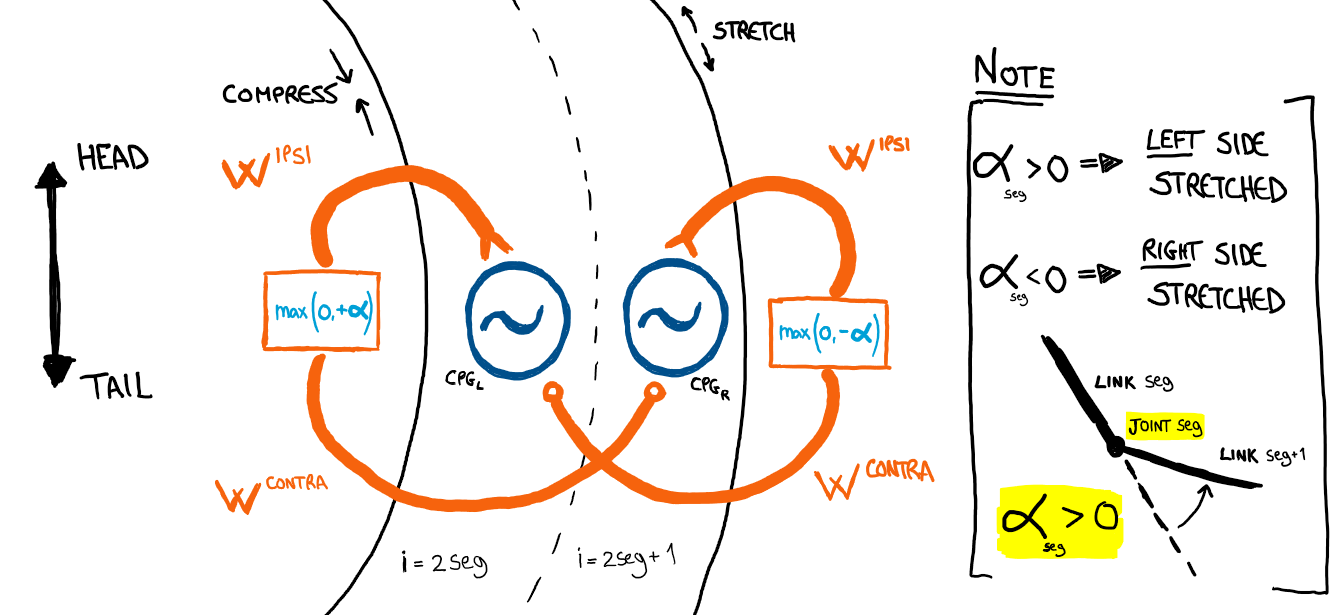
\includegraphics[width=\textwidth]{figures/CPG_scheme.png}}
  \end{subfigure}
  \caption{\label{fig:cpg_scheme} Schematics of the proprioceptive sensory feedback}
\end{figure}


The local proprioceptive feedback $s_i$ for oscillator $i$ is calculated as the sum of the effect
from ipsilateral and contralateral feedback, paying attention to the considered side.

For the LEFT oscillator at segment/joint $seg$ ($i = 2seg$):
\begin{equation}
  \label{eq:stot_left}
 s_i = W^{ipsi}max(0, +\alpha_{seg}) + W^{contra}max(0, -\alpha_{seg})
\end{equation}

For the RIGHT oscillator at segment/joint $seg$ ($i = 2seg + 1$):
\begin{equation}
  \label{eq:stot_right}
  s_i = W^{ipsi}max(0, -\alpha_{seg}) + W^{contra}max(0, +\alpha_{seg})
\end{equation}

Note that the feedback signal is only computed from the stretched side of the body, while
compression part is not considered.
For ease of implementation, we provide a reference feedback weight value $ws\_ref$,
computed as the inverse of the average joint angles that you used also for Project 1.
The value of $ws\_ref$ is provided in \fileref{util/zebrafish\_hyperparameters.py}.
In your code, you will modulate the reference value by two parameters
for the ipsilateral ($w_{ipsi}$) and contralateral ($w_{contra}$) components, according to

 \begin{eqnarray}
  \label{eq:s_weight}
  W^{ipsi}   = ws\_ref * w_{ipsi}    \quad \\
  W^{contra} = ws\_ref * w_{contra}
\end{eqnarray}

After including proprioceptive feedback, the oscillator equations have to be updated:


\begin{equation}
  \label{eq:damplitude}
  \dot{r}_i = a(R_i-r_i)+s_icos(\theta_i)
\end{equation}

with $ r_i $ the
oscillator amplitude, $ R_i $ the nominal amplitude, $\theta_i$ the oscillator phase.

\begin{equation}
  \label{eq:dphase}
  \dot{\theta}_i = 2 \pi f + \sum_j r_j w_{ij} sin(\theta_j - \theta_i - \phi_{ij}) - \frac{s_i}{R_i}sin(\theta)
\end{equation}

with $ f $ the frequency, $ r_i $ the
oscillator amplitude, $ w_ij $ the coupling weights, $\theta_i$ the oscillator phase.

\textbf{Correction of project 1: }
Note that in Project 1 Eqn.4 and Eqn.5, we only implemented the coupling from left to right side,
which worked in open-loop. For a closed-loop CPG, we need the coupling to be mutual:

\begin{equation}
  \label{eq:dcw}
  w_{ij} =
    \begin{cases}
    w_{body2body},& \text{if } |i-j|=2 \\
    w_{body2body\_contralateral}, & \text{if }  j-i=1 \text{ and } i\%2=0\\
    w_{body2body\_contralateral}, & \text{if }  i-j=1 \text{ and } i\%2=1 \text{ \textbf{(mutual)} }\\
    0, & \text{otherwise} \\
    \end{cases}
\end{equation}

\begin{equation}
  \label{eq:phicw}
  \phi_{ij} =
    \begin{cases}
    sign(i-j)\cdot\frac{\phi_{body\_total}}{n_{joints}-1},& \text{if } |i-j|=2 \\
    sign(i-j)\cdot\pi,&  \text{if }  j-i=1 \text{ and } i\%2=0\\
    sign(i-j)\cdot\pi,& \text{if }   i-j=1 \text{ and } i\%2=1 \text{ \textbf{(mutual)} }\\
    0, & \text{otherwise} \\
    \end{cases}
\end{equation}

\textbf{\underline{Question 5.1} Update \fileref{abstract\_oscillator\_controller.py} to implement the stretch feedback.}

\textbf{\underline{Question 5.2} Test your implementation by running the network using \fileref{exercise5.py} with default values $W^{ipsi}=0.25 * ws_{ref}$ and $W^{contra}=-0.25 * ws_{ref}$. Plot the oscillator phases evolution, oscillator amplitudes evolution, motor output and motor output difference evolution, and the zebrafish joint angles evolution vs time. Observe the result and analyze how it changes compared to open-loop CPGs}.

\textbf{\underline{Answer 5.2:}} 
As a premise, we ran the simulations with the pre-set initial phases, that is a gradient of phases from 0 to $2\pi$ rostro-caudally.
Oscillator phases grow linearly in time, suggesting synchronization between oscillators, as it was the case in the open loop case. Oscillator amplitudes, on the other hand, have a different trend compared to the previous case. Here, oscillations are not converging to a constant value, but every joint shows a different asymptotic value and oscillatory trend, due to the last term of the equation \ref{eq:dphase}. Left and right motor output evolution are coherent between them and show an ondulatory pattern over time, with  variable amplitude between joints. Lateral difference between motor output is coherent with what is expected, summing constructively. Joint angles evolution plot show an initial transient form, needed to reach the limit cycle, and then a stable regime, where each joint has its own joint angle ondulatory excursion over time, similarly to the ones found in the open loop case.

\begin{figure}[H]
    \centering
    \begin{minipage}{0.48\textwidth}
        \centering
        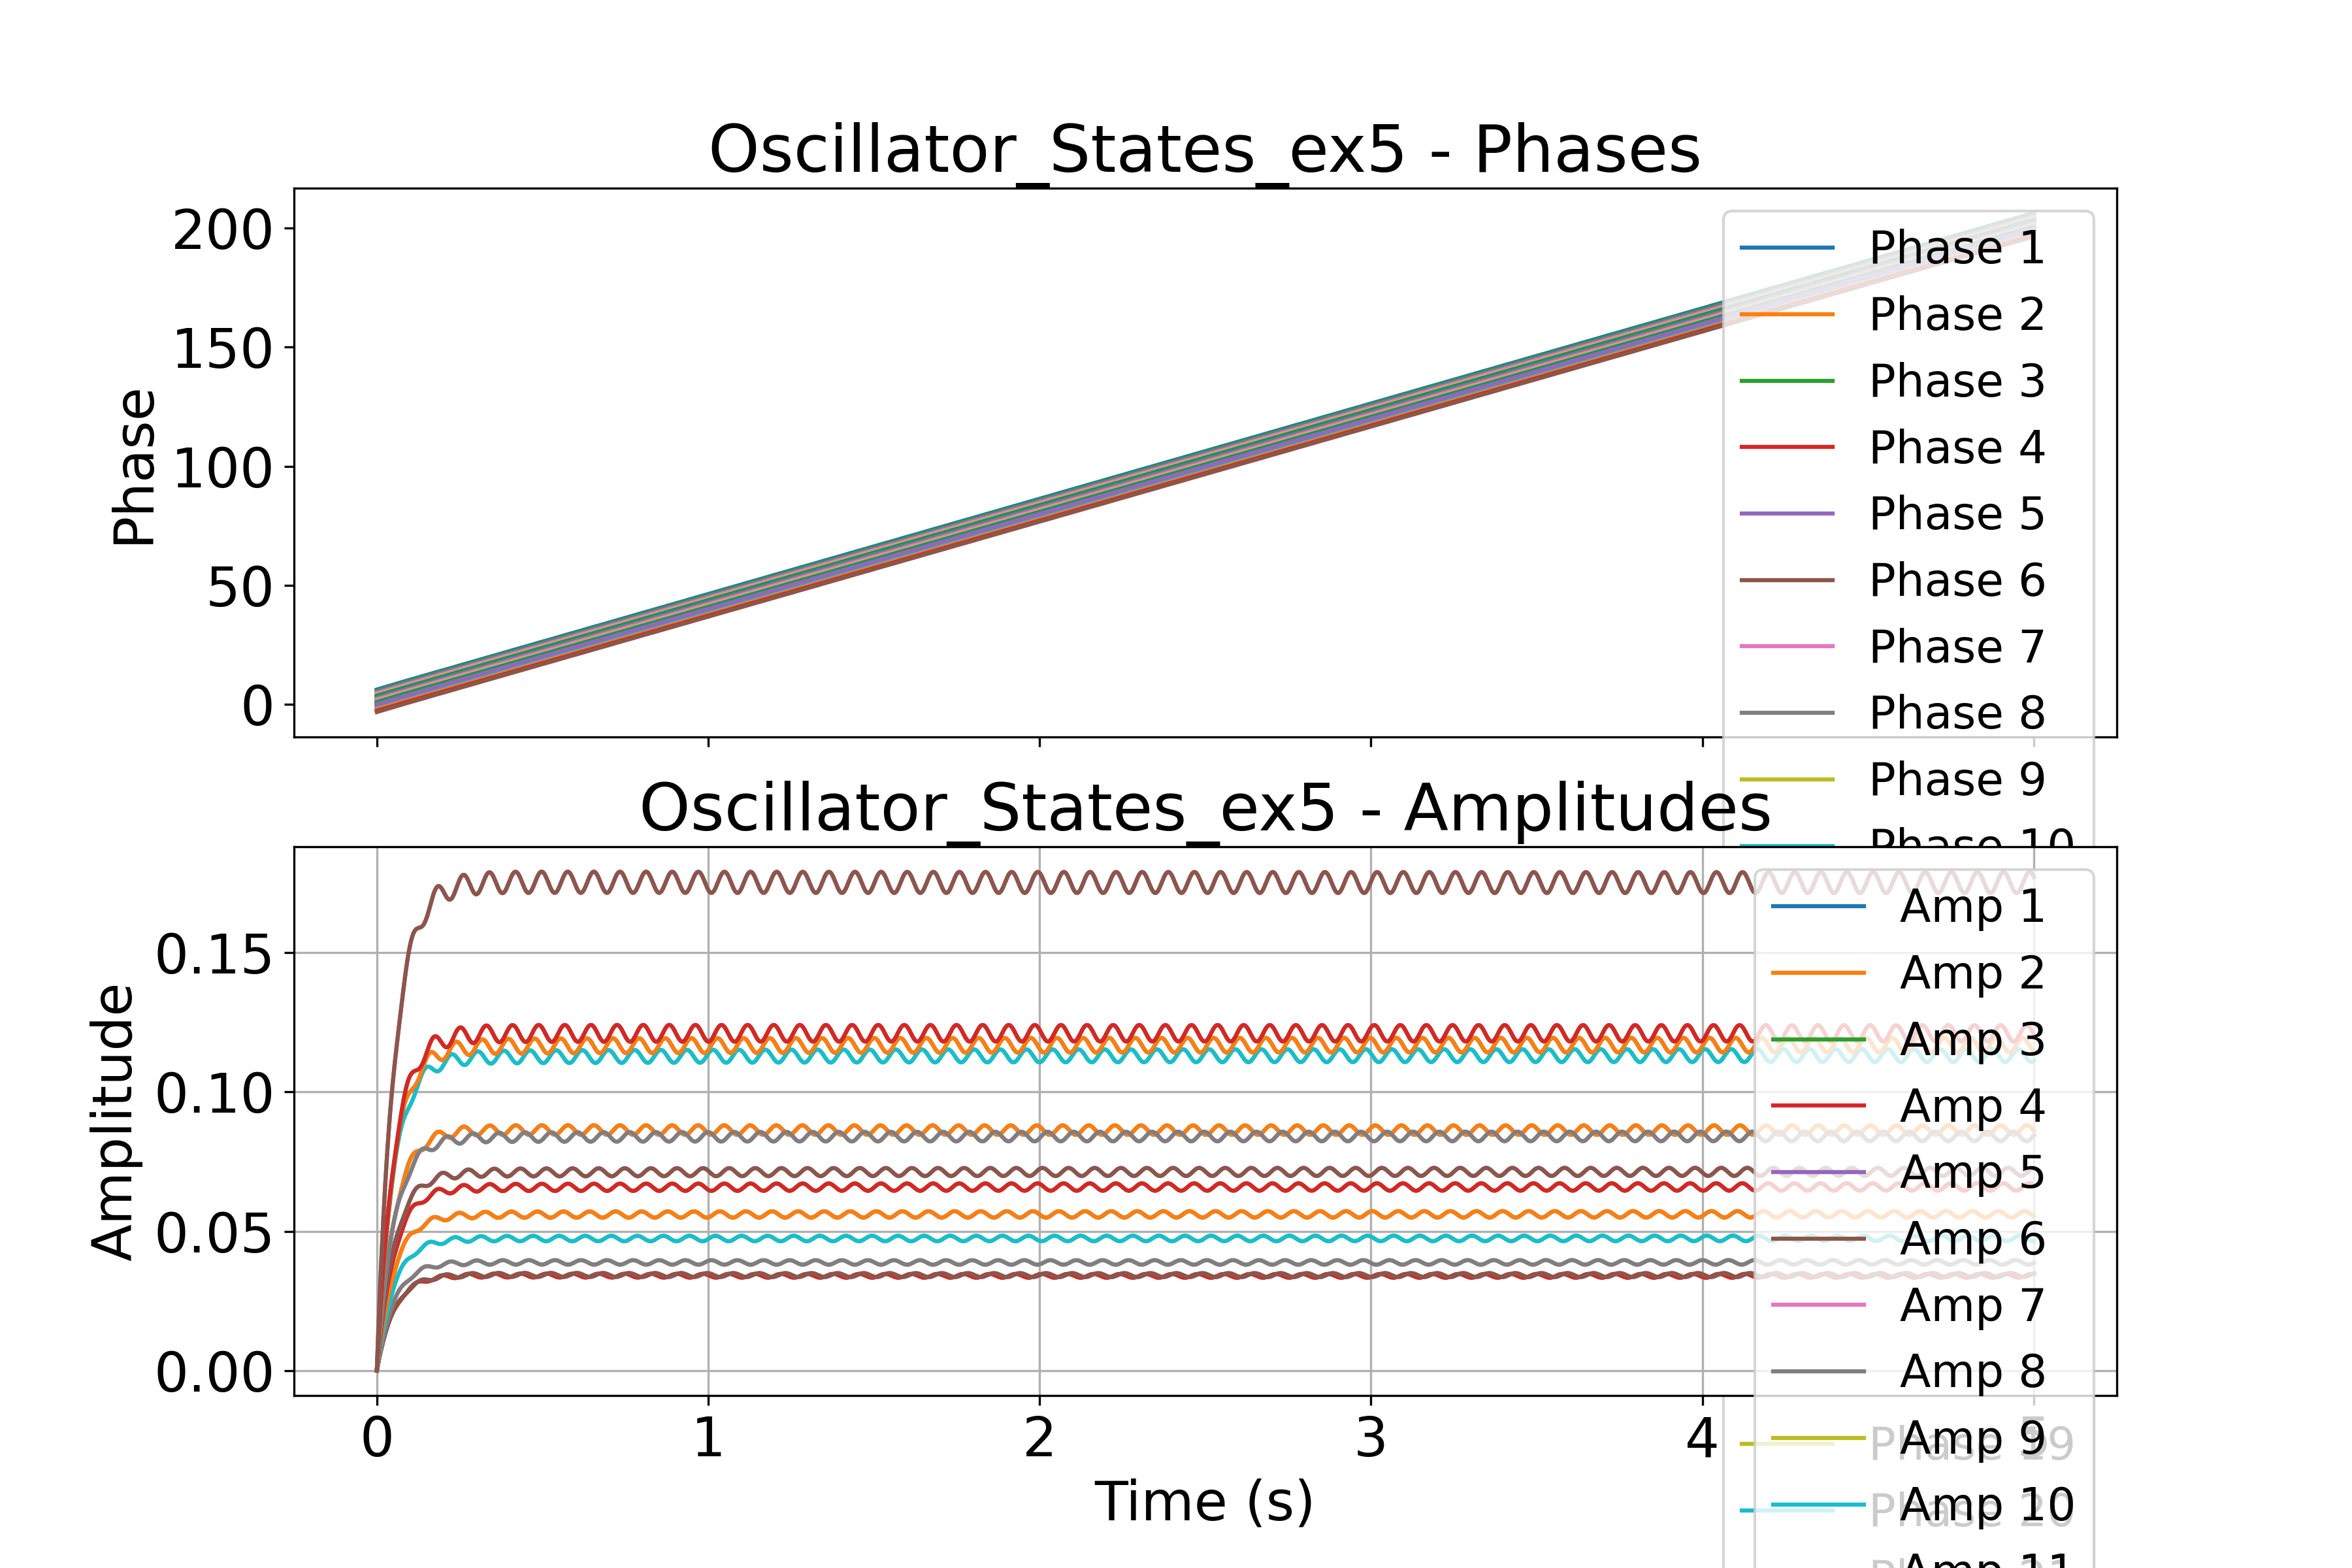
\includegraphics[width=\linewidth]{our_figures/Oscillator_States_ex5.png}
        \caption{Oscillator phases and amplitudes evolution}
        \label{fig:Oscillator_States_ex5}
    \end{minipage}\hfill
    \begin{minipage}{0.48\textwidth}
        \centering
        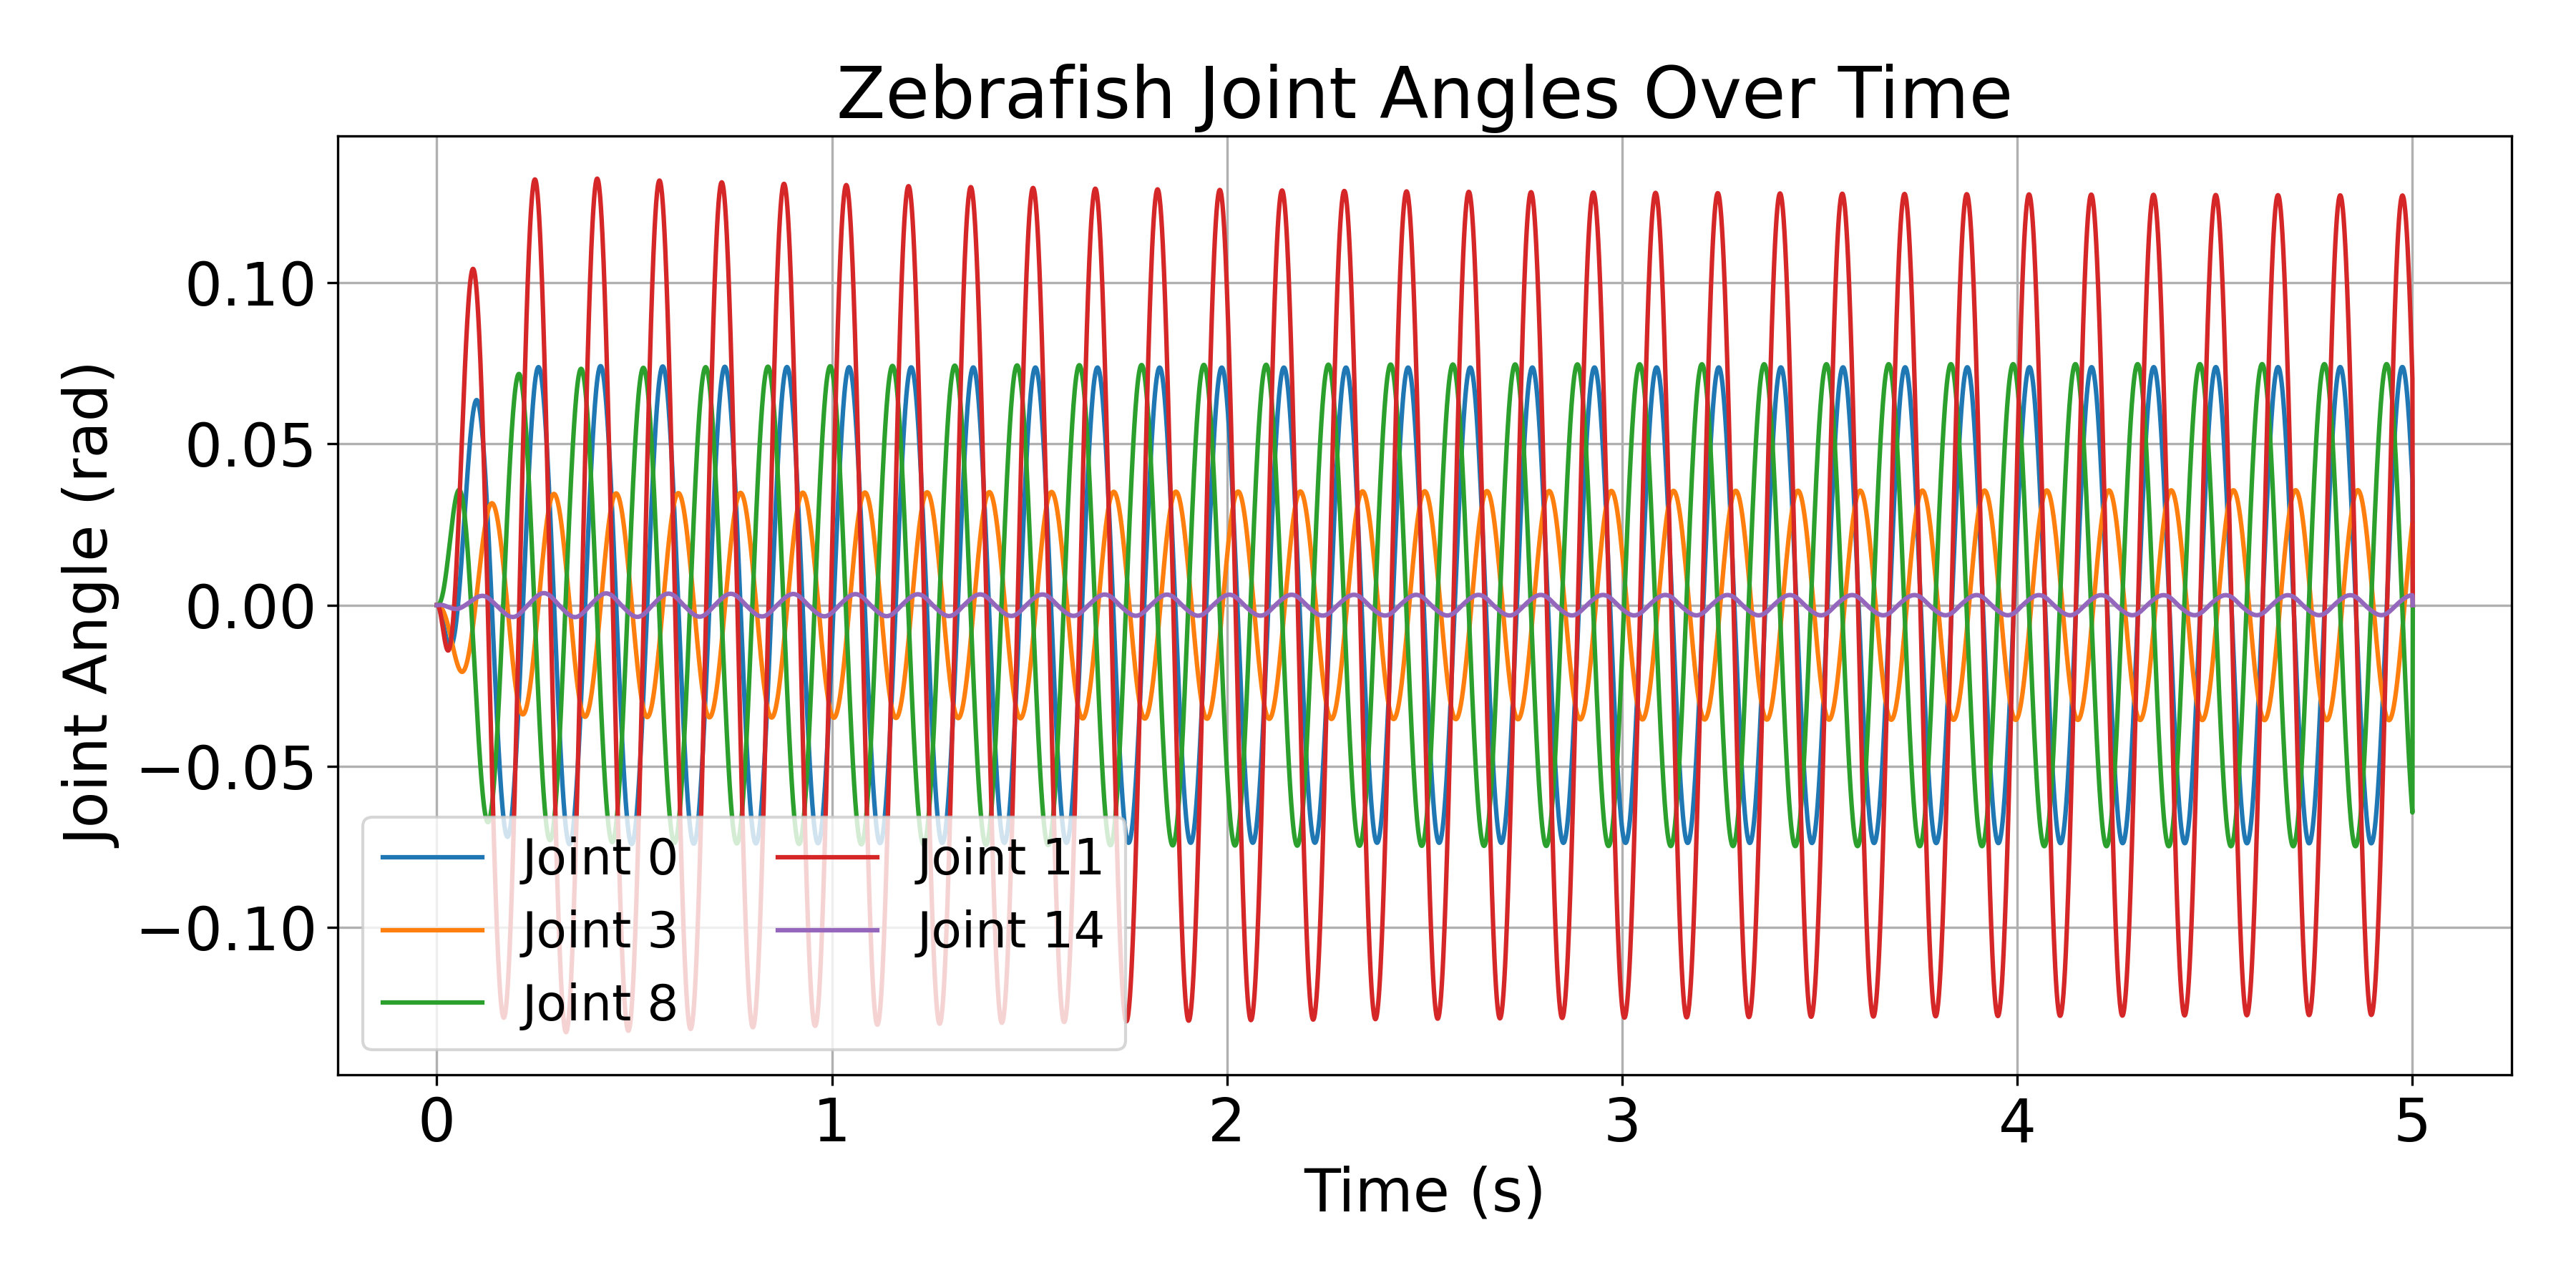
\includegraphics[width=\linewidth]{our_figures/Joint_Angles_ex5.png}
        \caption{Joint angles evolution}
        \label{fig:Joint_Angles_ex5}
    \end{minipage}
\end{figure}

\begin{figure}[H]
    \centering
    \begin{minipage}{0.38\textwidth}
        \centering
        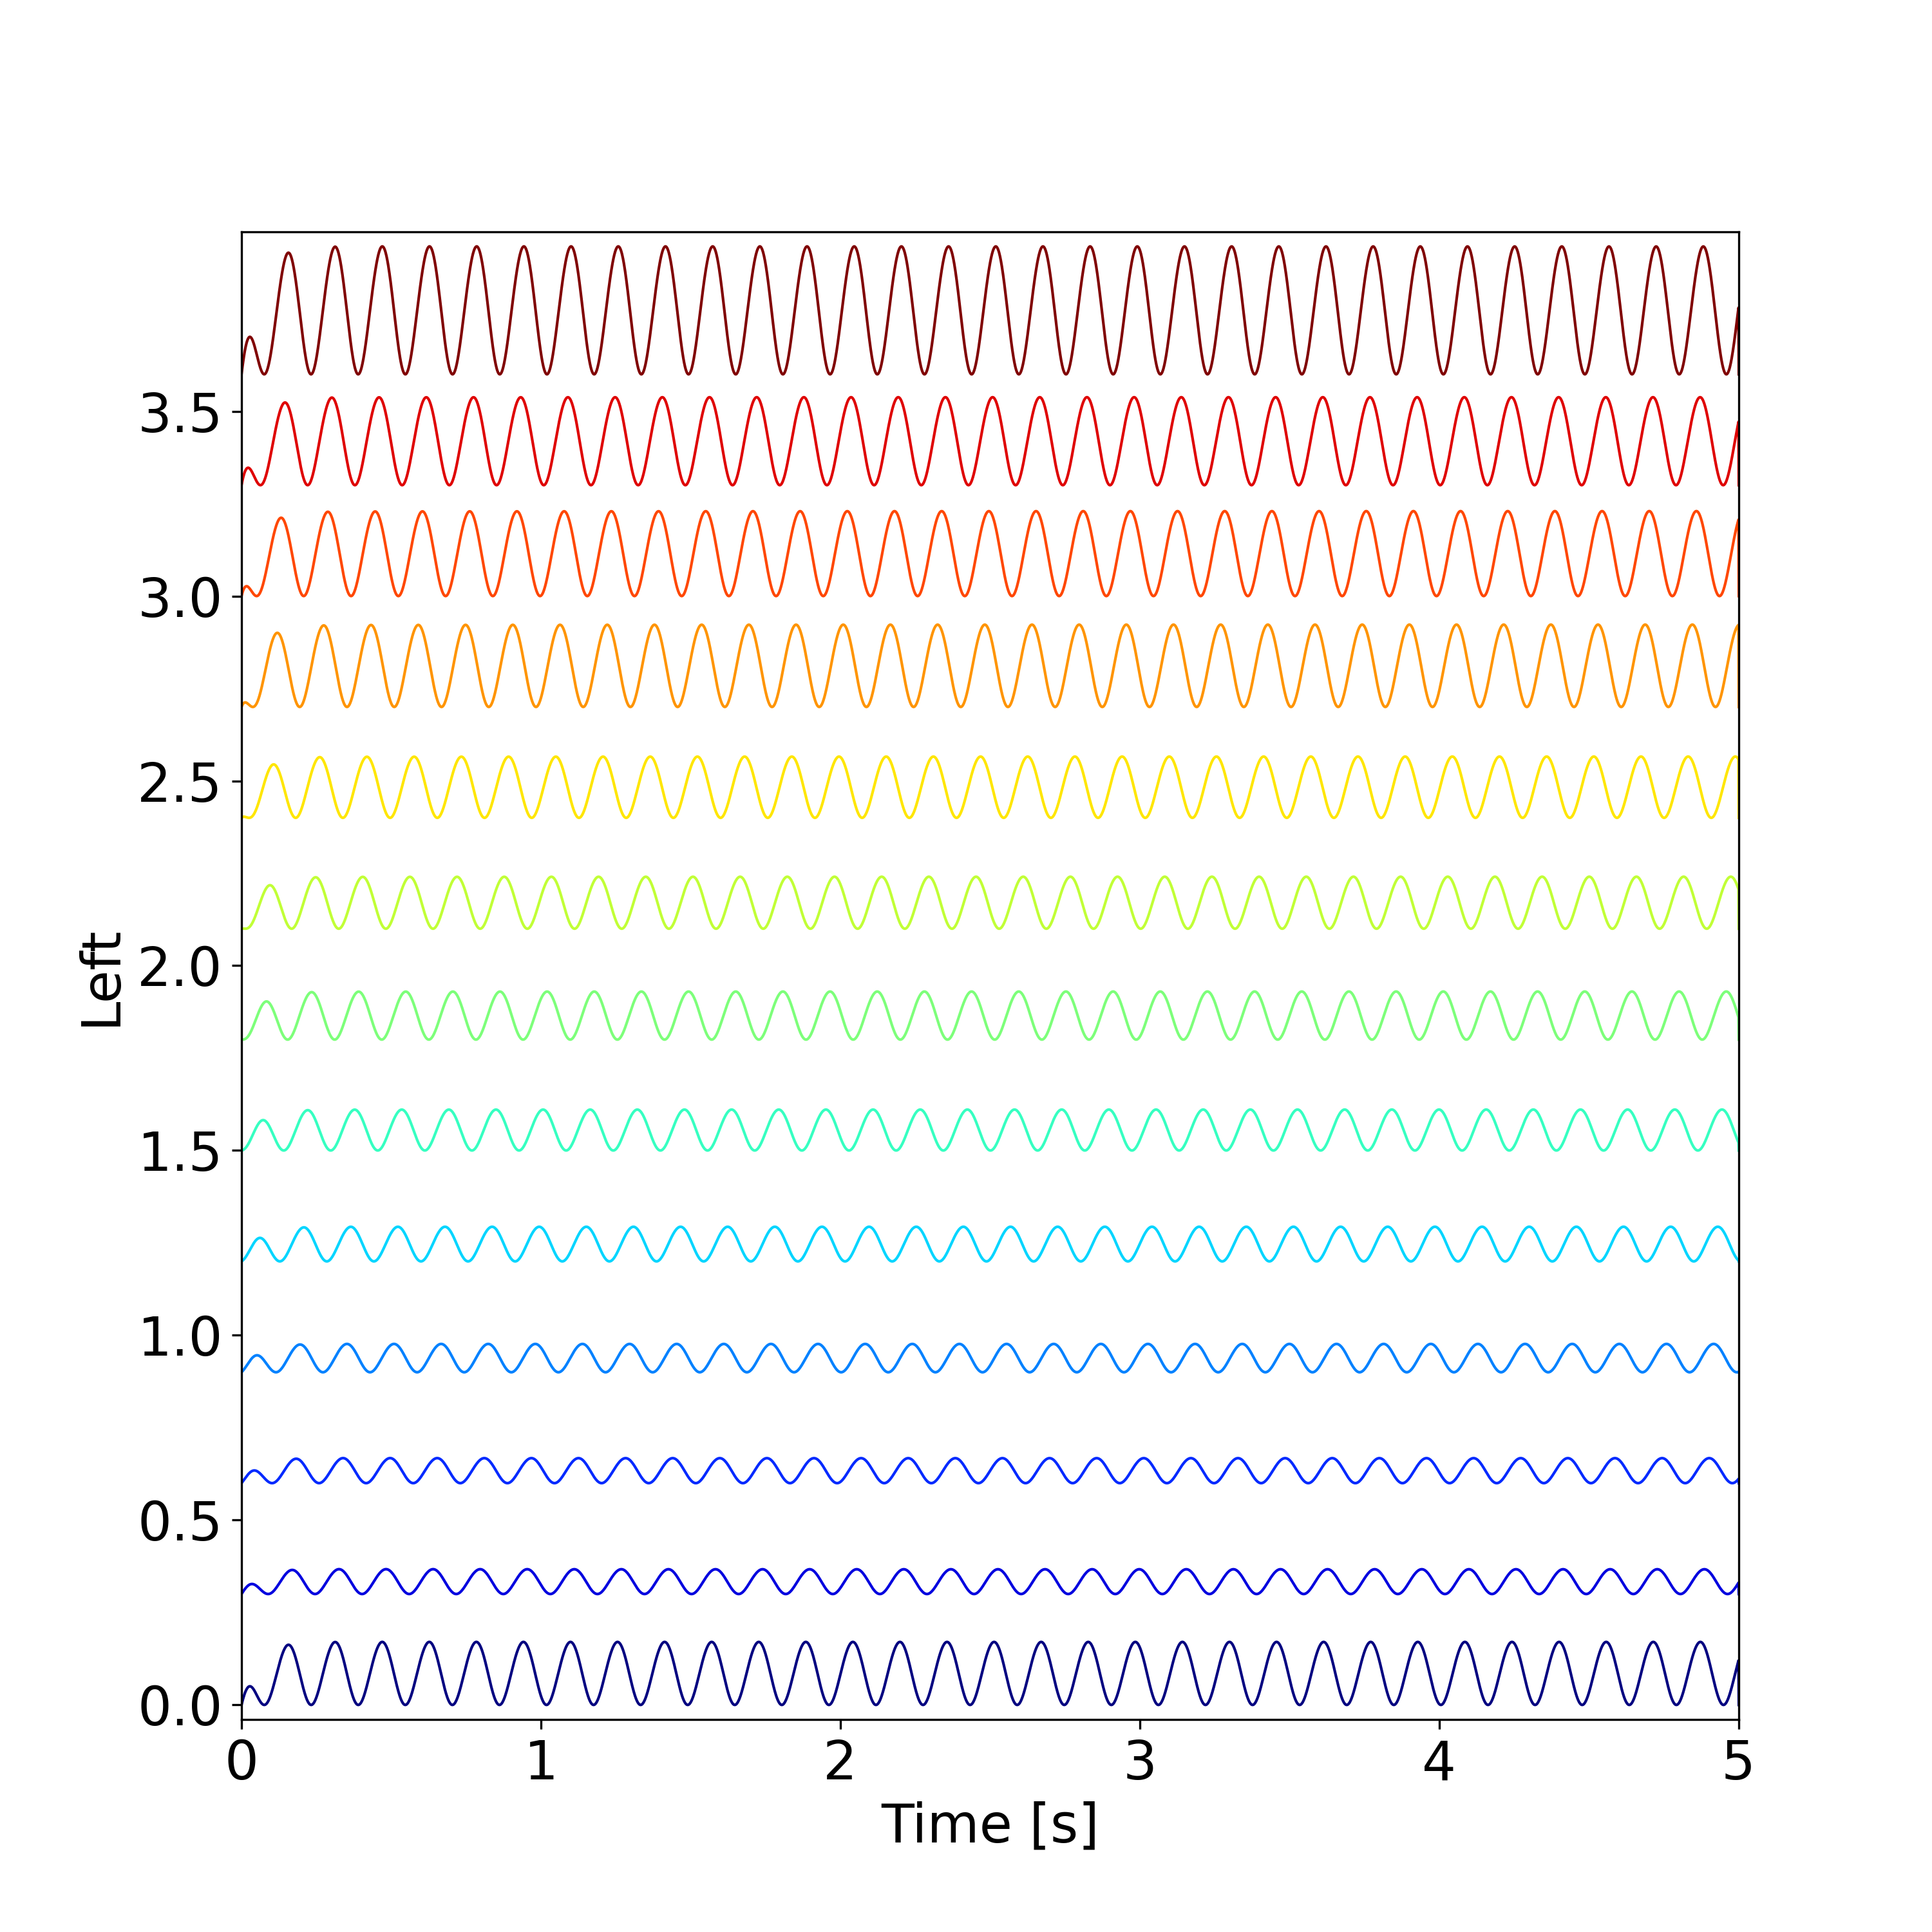
\includegraphics[width=\linewidth]{our_figures/Motor_ex5 _Left.png}
        \caption{Motor output left}
        \label{fig:Motor_ex5_Left}
    \end{minipage}
    \hfill
    \begin{minipage}{0.38\textwidth}
        \centering
        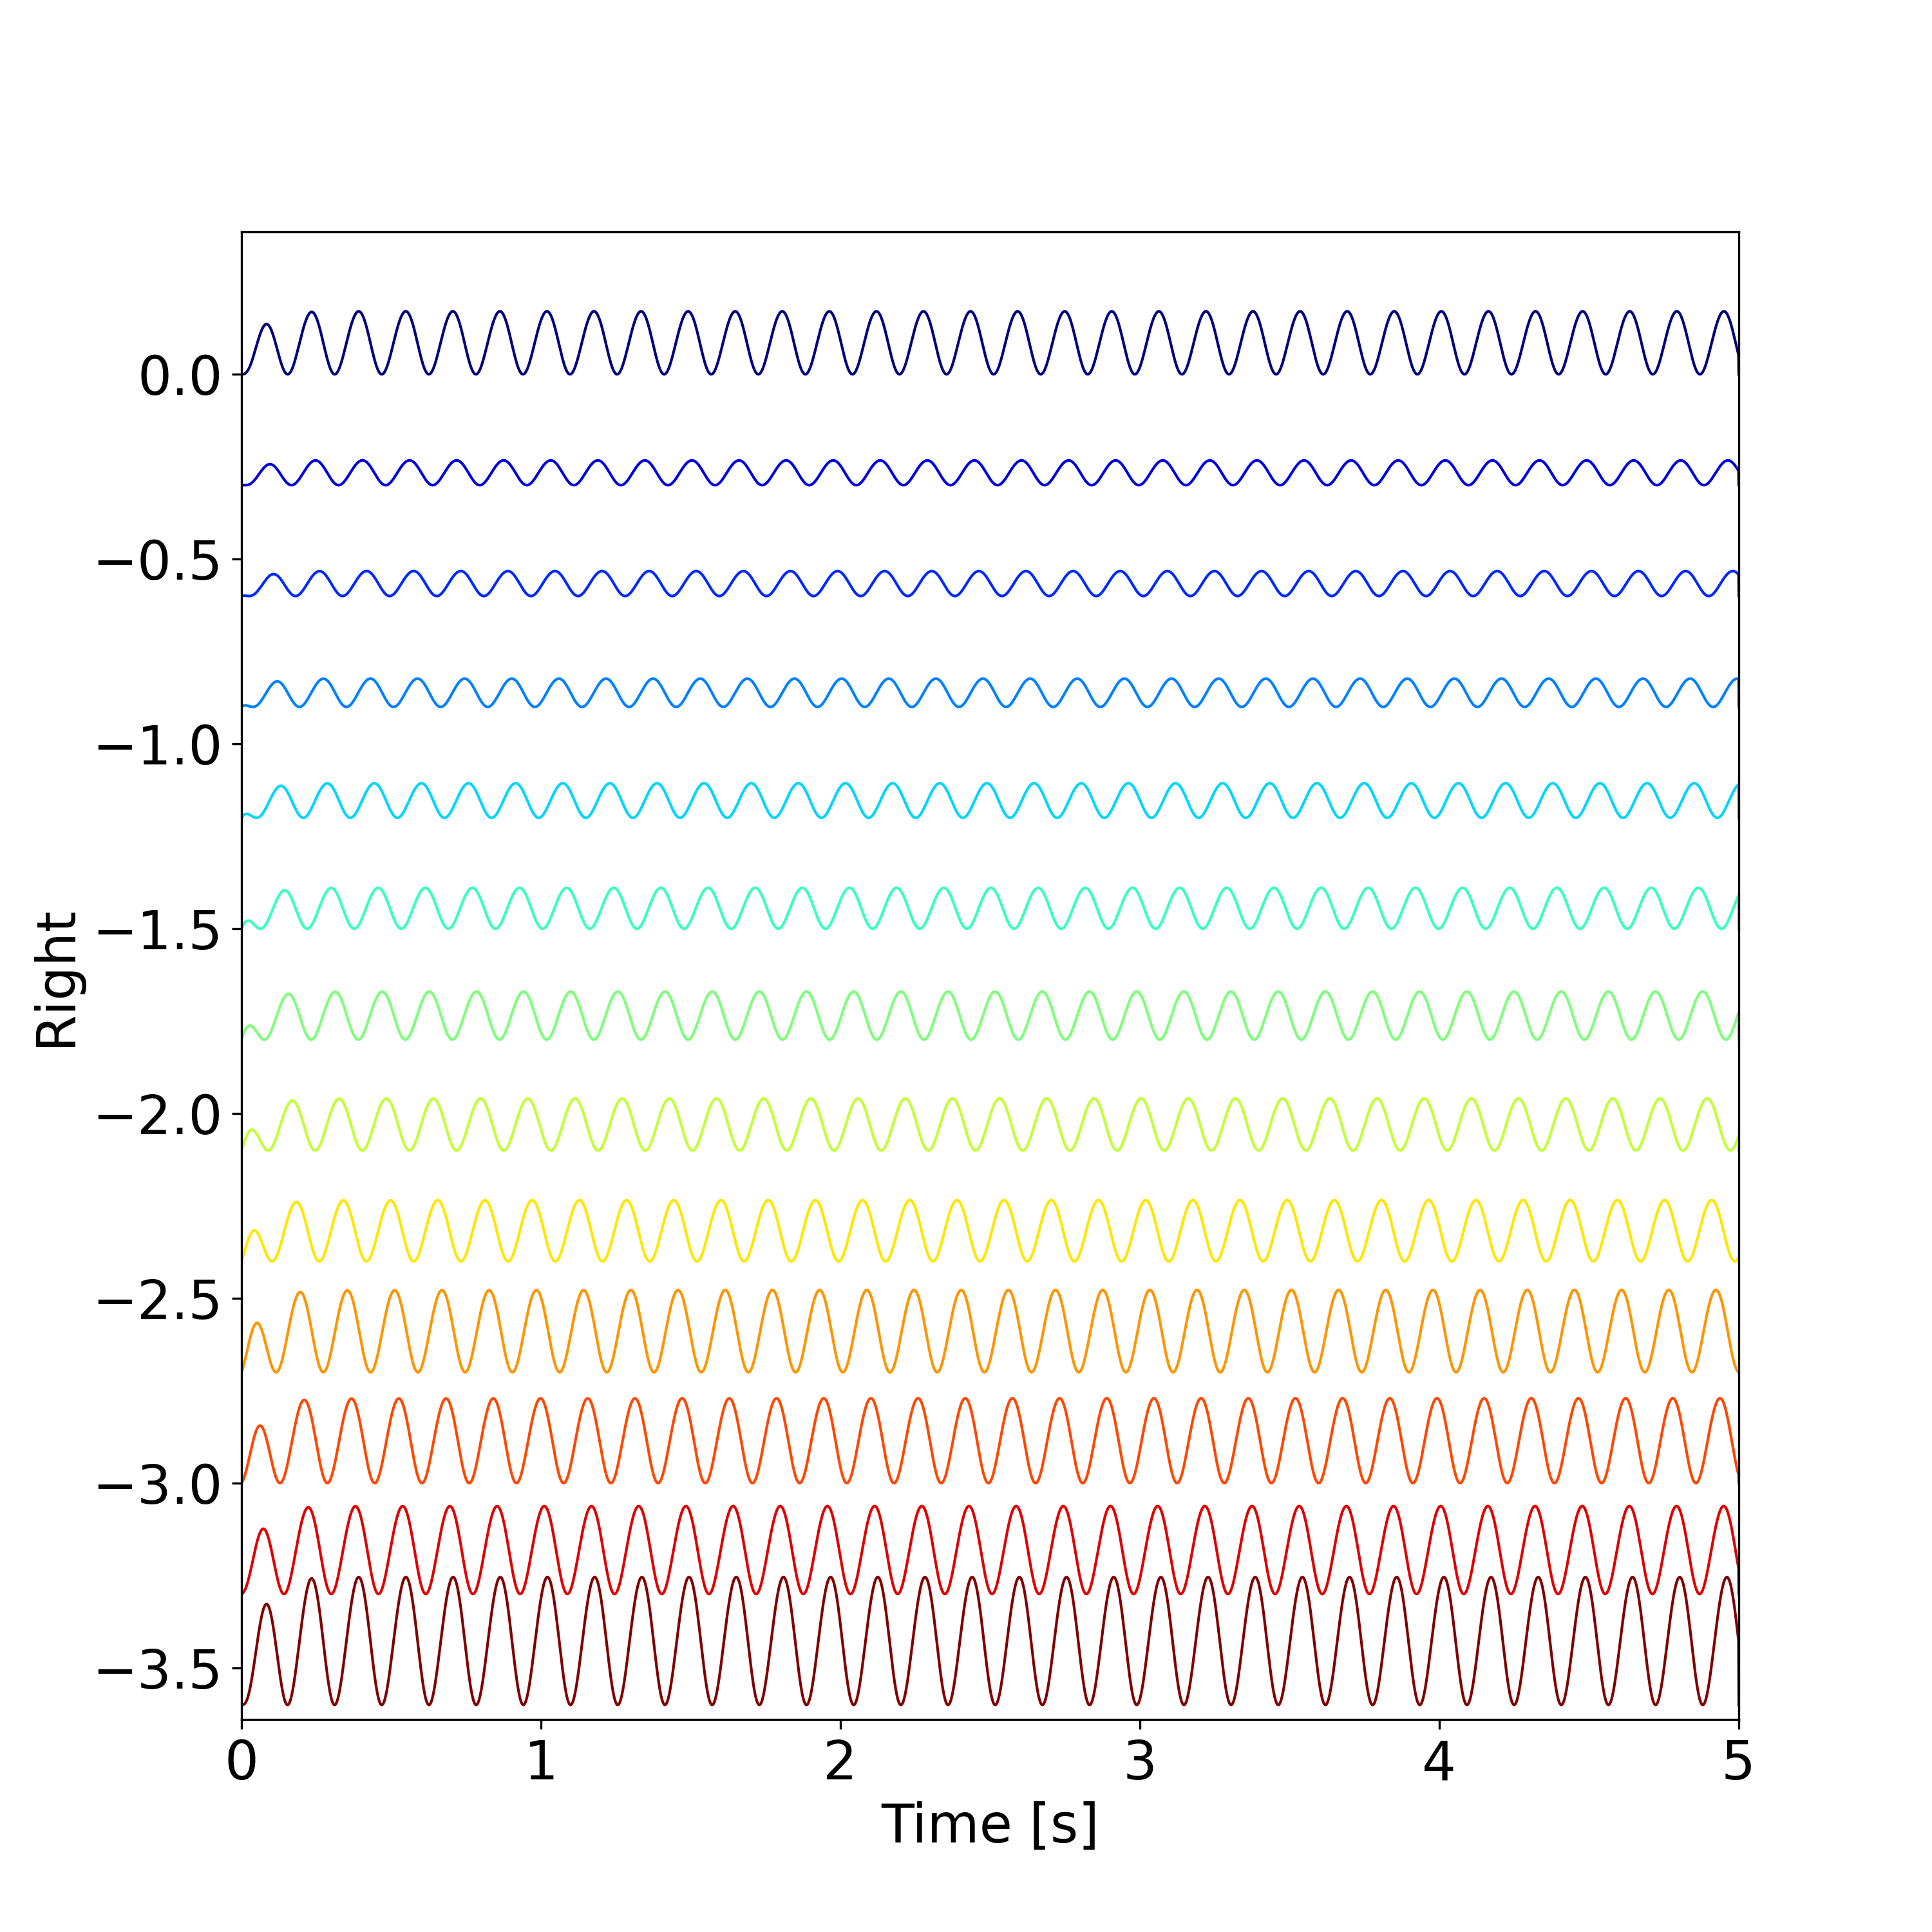
\includegraphics[width=\linewidth]{our_figures/Motor_ex5 _Right.png}
        \caption{Motor output right}
        \label{fig:Motor_ex5_Right}
    \end{minipage}
\end{figure}


\begin{figure}[H]
    \centering
    \begin{minipage}{0.38\textwidth}
        \centering
        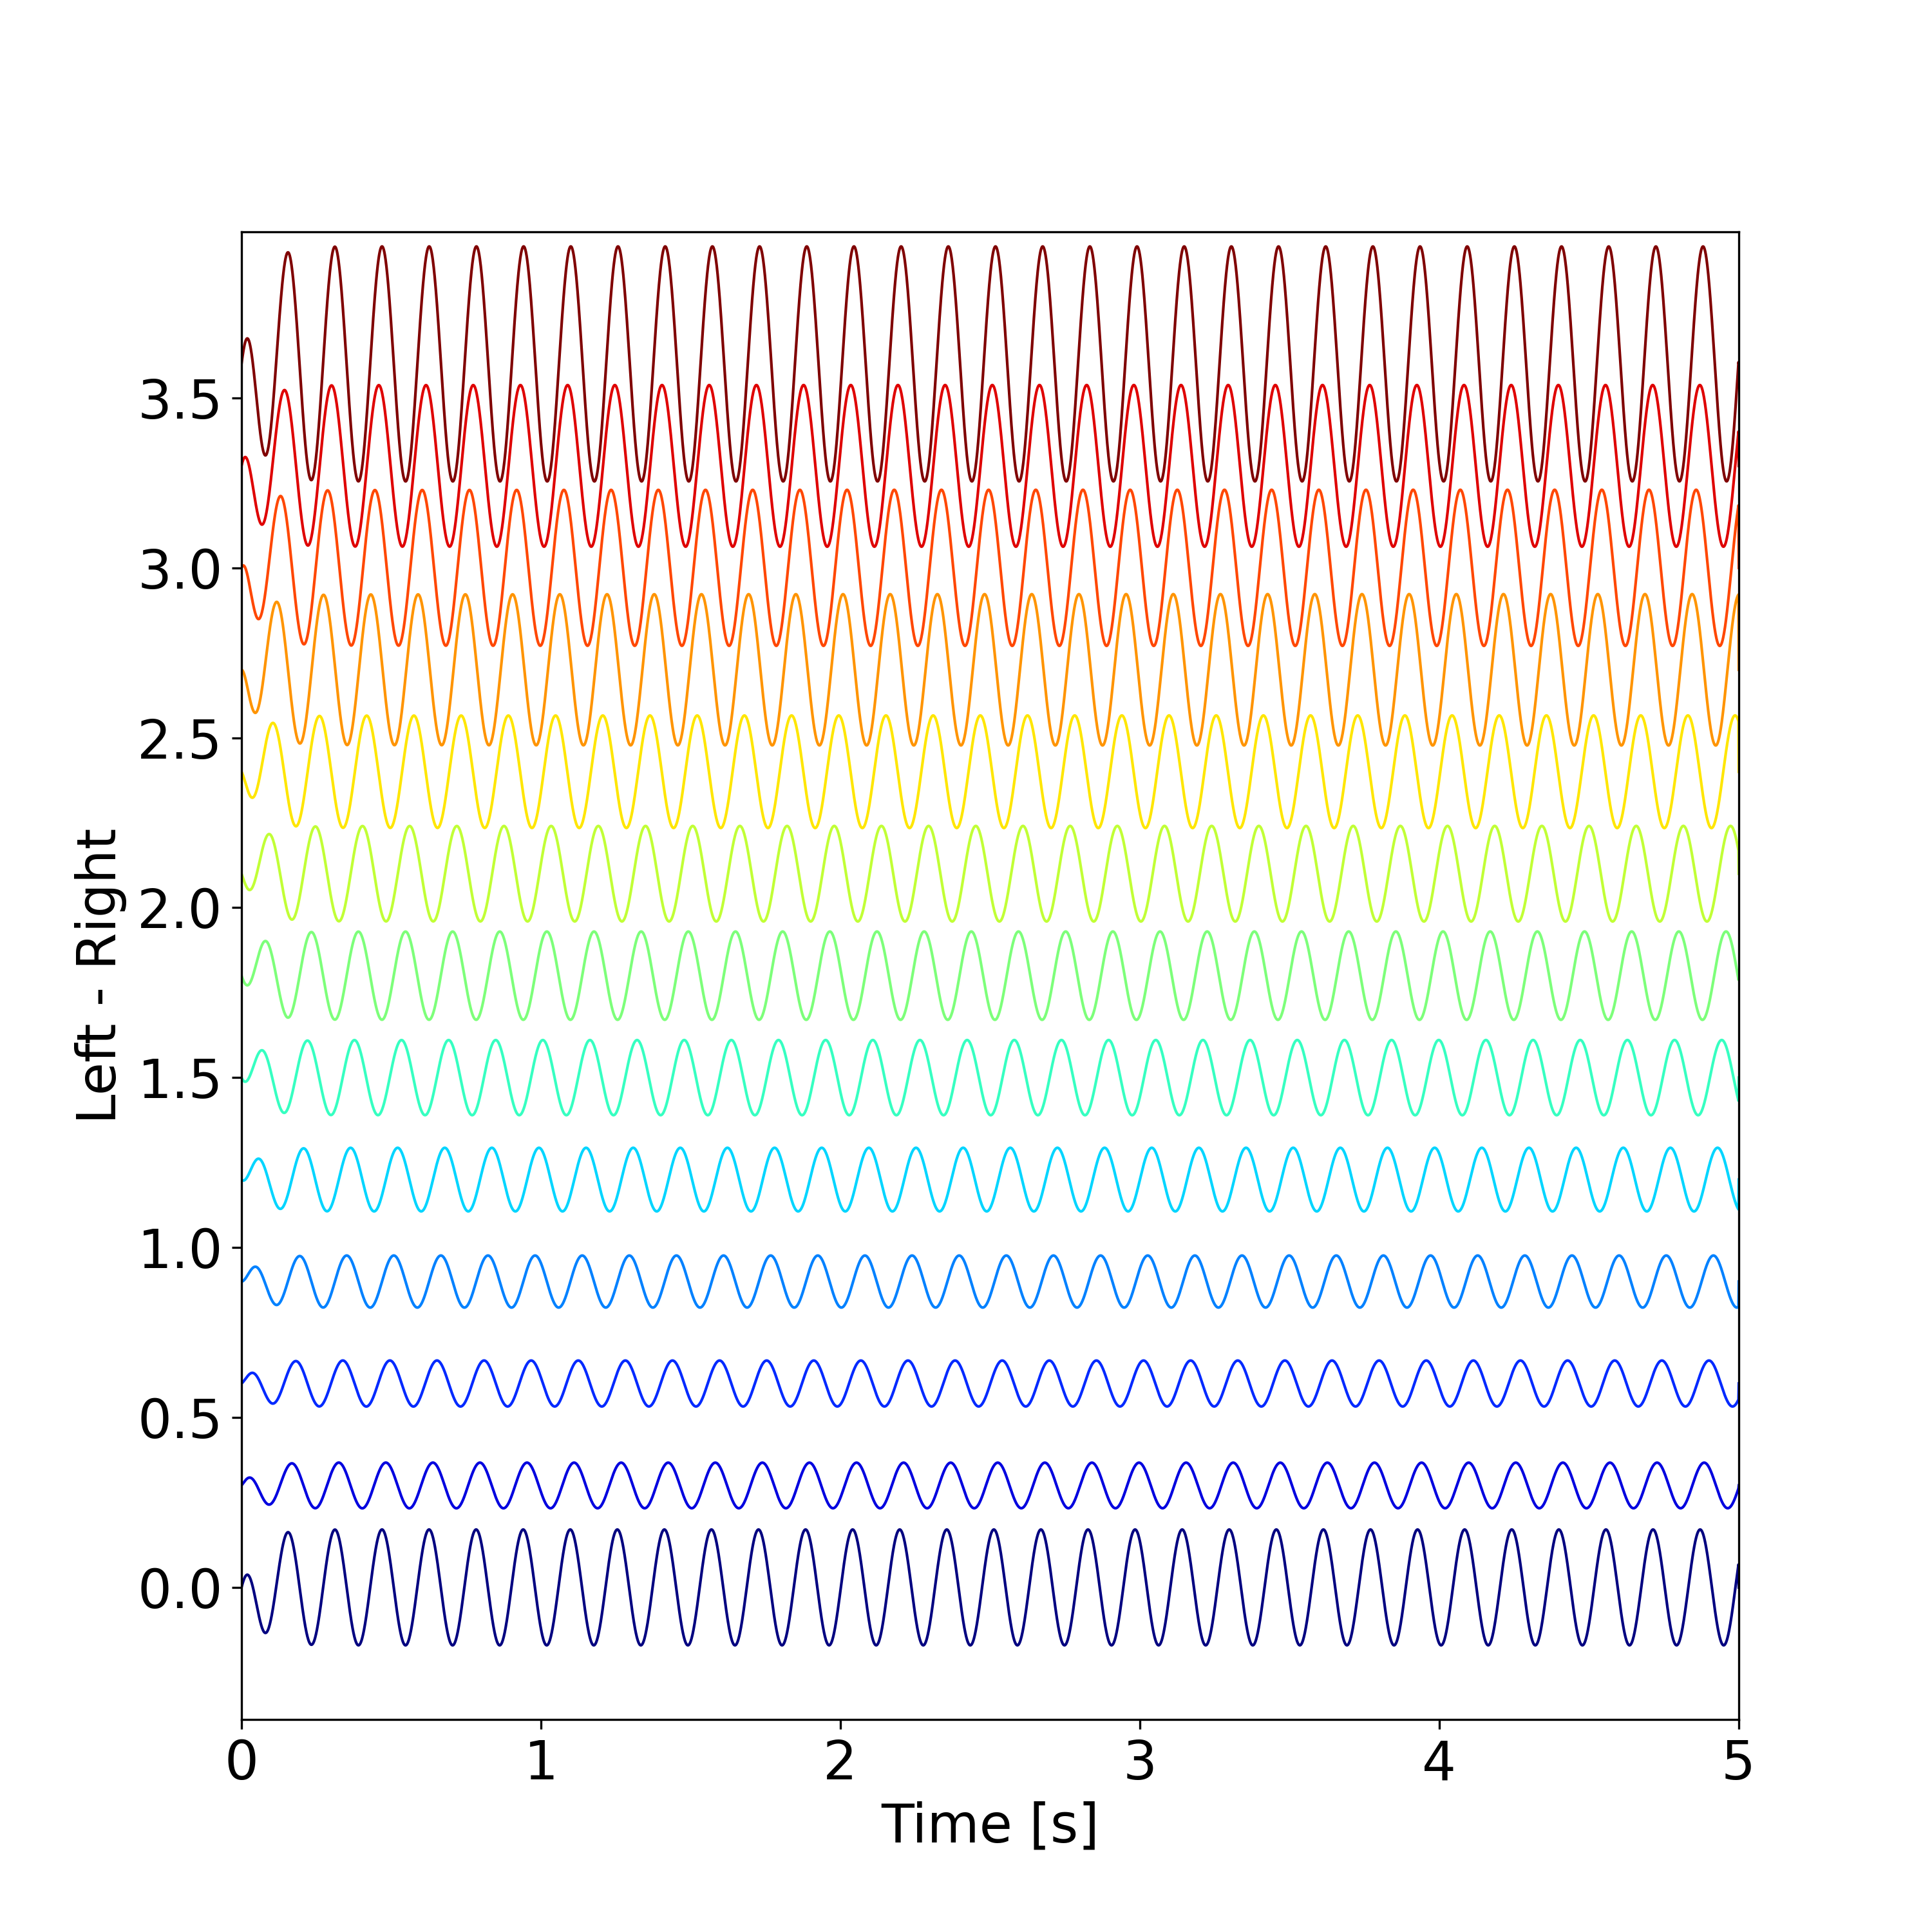
\includegraphics[width=\linewidth]{our_figures/Lateral_Diff_ex5 _Left - Right.png}
        \caption{Motor output lateral difference left - right}
        \label{fig:Lateral_Diff_ex5_Left-Right}
    \end{minipage}
    \hfill
    \begin{minipage}{0.38\textwidth}
        \centering
        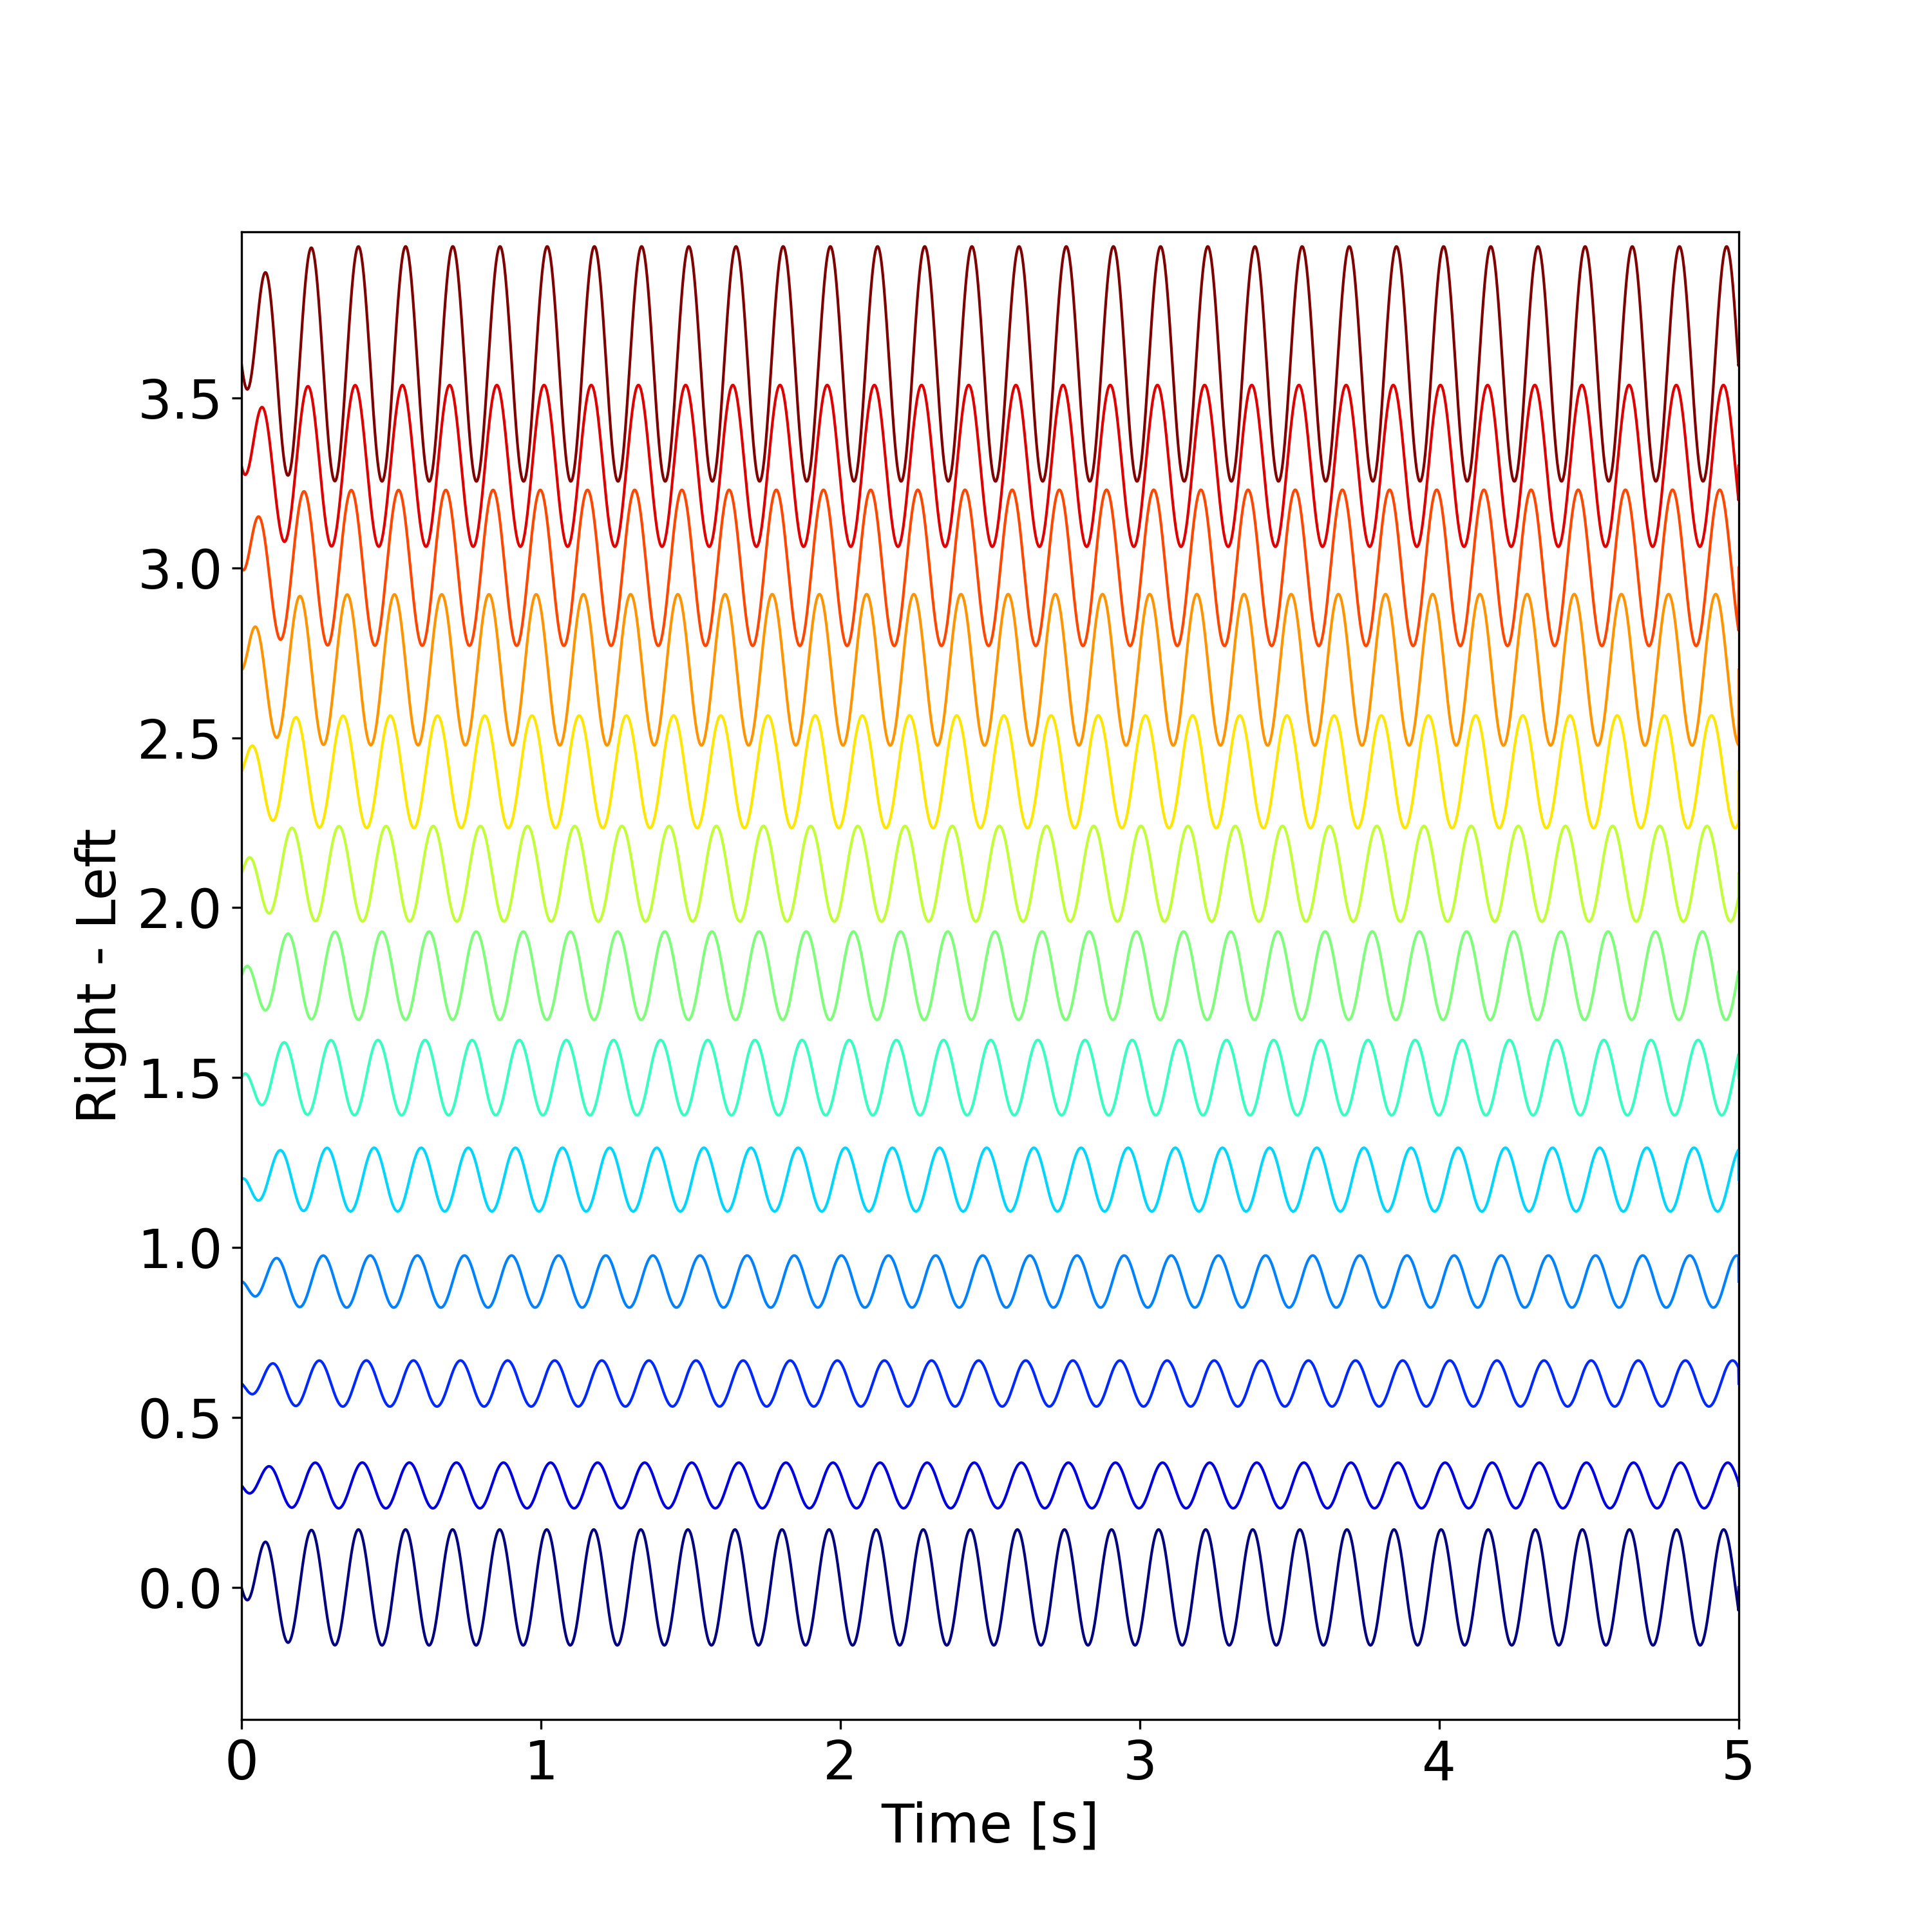
\includegraphics[width=\linewidth]{our_figures/Lateral_Diff_ex5 _Right - Left.png}
        \caption{Motor output lateral difference right - left}
        \label{fig:Lateral_Diff_ex5_Right-Left}
    \end{minipage}
\end{figure}


\textbf{\underline{Question 5.3} Report the controller and mechanical metrics of the simulation.  Record a video of the zebrafish swimming for 10s}.

\textbf{\underline{Answer 5.3:} }

\begin{table}[h!]
\centering
\begin{tabular}{|l|l|}
\hline
\textbf{Metric} & \textbf{Value} \\
\hline
CPG Amplitude Gain & \makecell[r]{[0.00824, 0.00328, 0.00328, 0.00370, 0.00451,\\
                                   0.00534, 0.00628, 0.00680, 0.00803, 0.01084,\\
                                   0.01115, 0.01149, 0.01655]} \\
CPG Frequency Gain & 0.6 \\
CPG Frequency Offset & 0.6 \\
Feedback Weights (ipsilateral) & $0.25 \cdot ws\_ref$ \\
Feedback Weights (contralateral) & $-0.25 \cdot ws\_ref$ \\
\hline
Neural Frequency & 6.32996 \\
Neural Mean IPL & 0.08547 \\
Neural TWL & 1.53849 \\
Neural AMP & 0.15682 \\
Mean Mechanical Frequency & 6.33207 \\
Forward Speed & 0.01694 \\
Lateral Speed & 4.34e-07 \\
Mechanical Torque & 0.00107 \\
Mechanical Energy & 2.05e-06 \\
Cost of Travel & 4.03e-05 \\
Mean Joint Amplitude & 0.06485 \\
Mechanical IPL & 0.08052 \\
Mechanical TWL & 1.44943 \\
\hline
\end{tabular}
\caption{Computed metrics and parameters}
\label{tab:metrics_full}
\end{table}

\textbf{\underline{Question 5.4} Test different feedback weight values for ipsilateral and contralateral feedback connections in \fileref{exercise6.py}. Keep $w^{ipsi}=0$ and test $w^{contra}$ in range [-1,1] scaled by $ws\_ref$. Keep $w^{contra}=0$ and test $w^{ipsi}$ in range [-1,1] scaled by $ws\_ref$. $ws\_ref$ is the inverse of average joint amplitudes (provided in the code). Plot the neural controller (neural frequency, total wave lag) and mechanical metrics (cost of transport, energy consumption, forward speed, joint amplitudes, sum of torques) as a function of different ipsilateral and contralateral feedback strengths.}.

\textbf{\underline{Answer 5.4:}}

\begin{figure}[H]
    \centering
    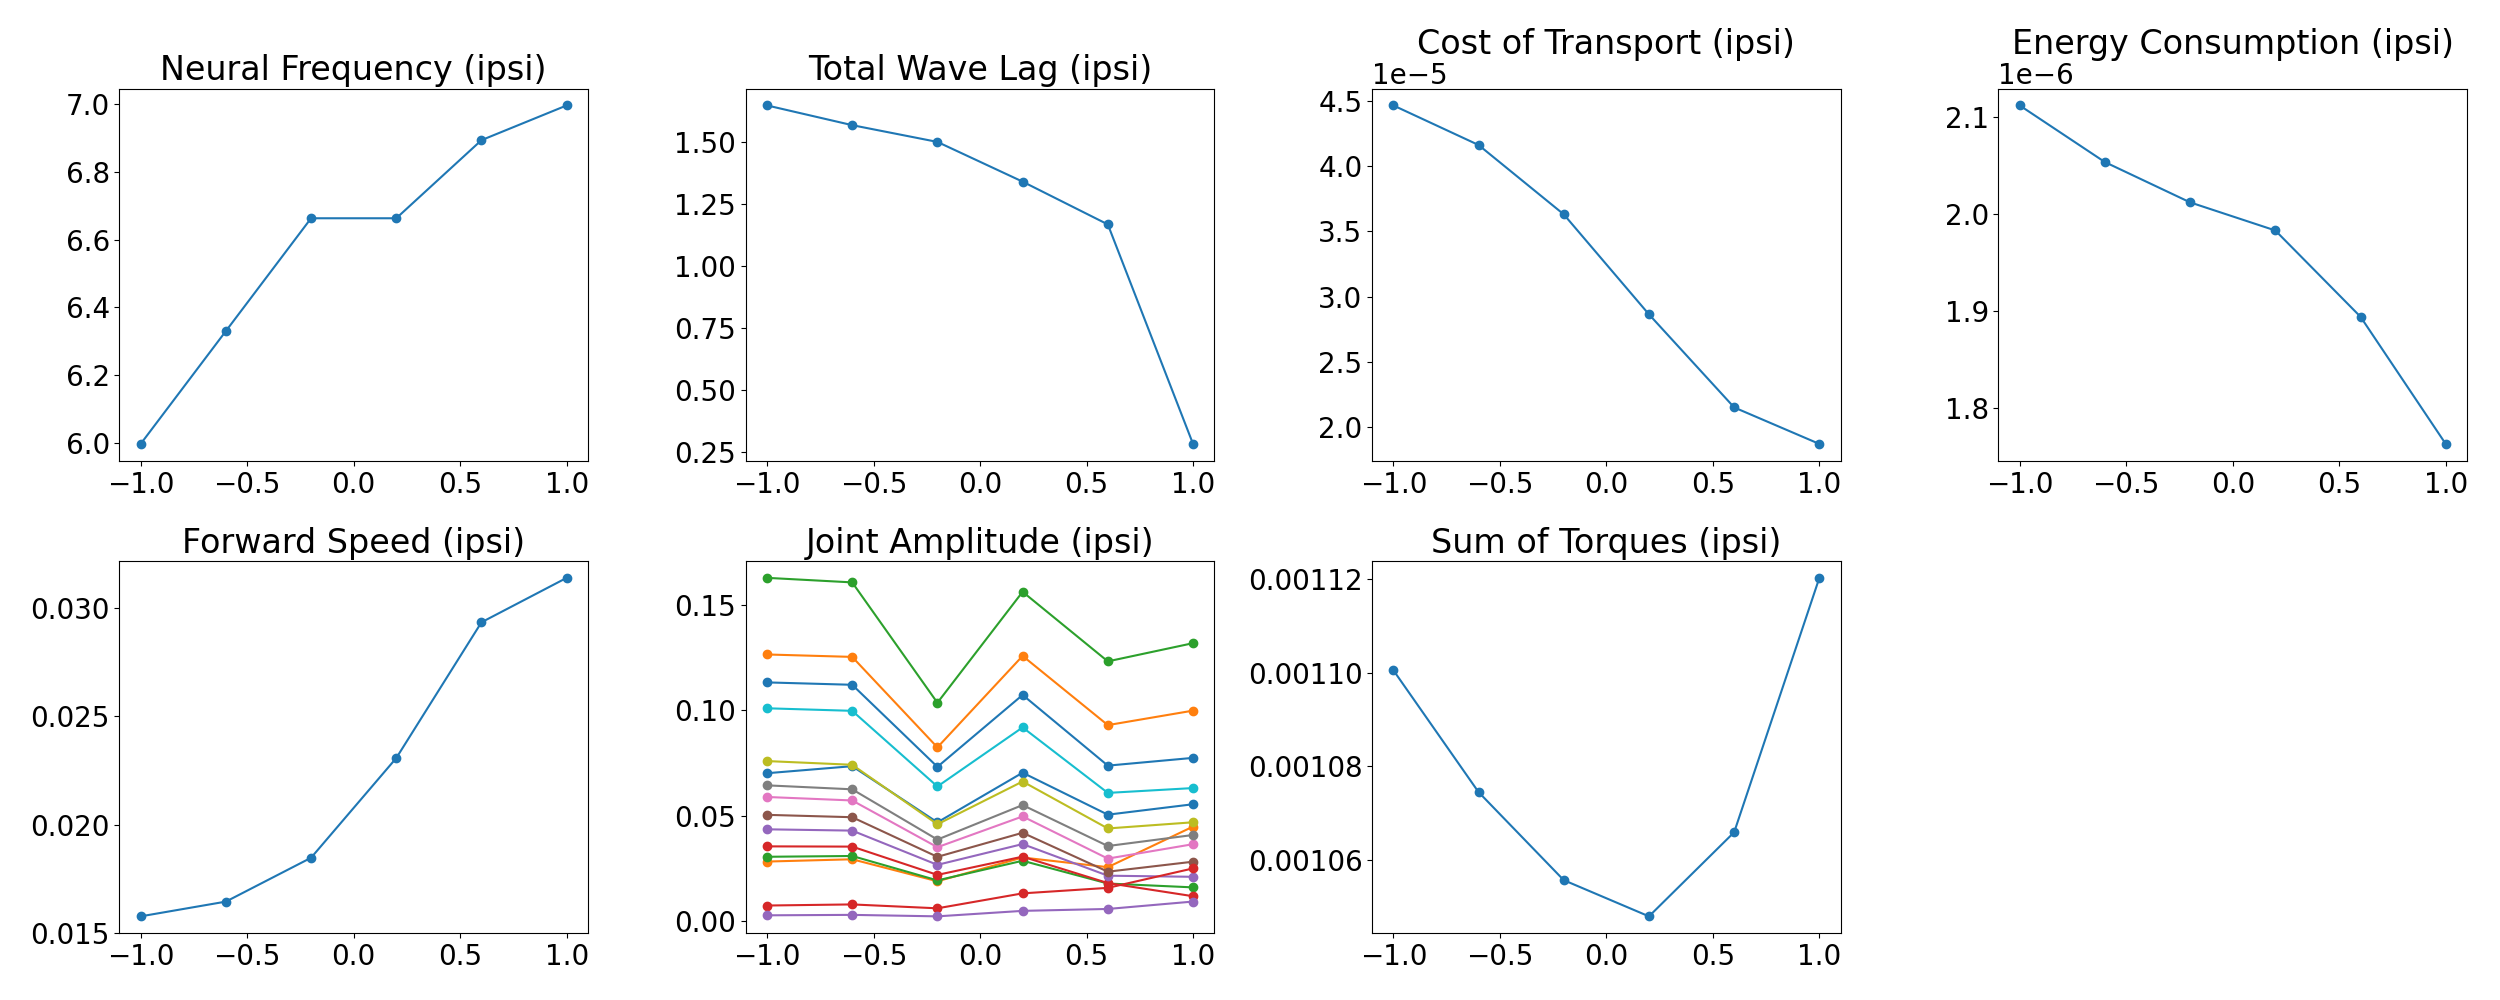
\includegraphics[width=0.8\linewidth]{our_figures/metrics_ipsi_variation.png}
    \caption{Controller and mechanical metrics depending on ipsilateral feedback strengths}
    \label{fig:metrics_ipsi_variation}
\end{figure}

\begin{figure}[H]
    \centering
    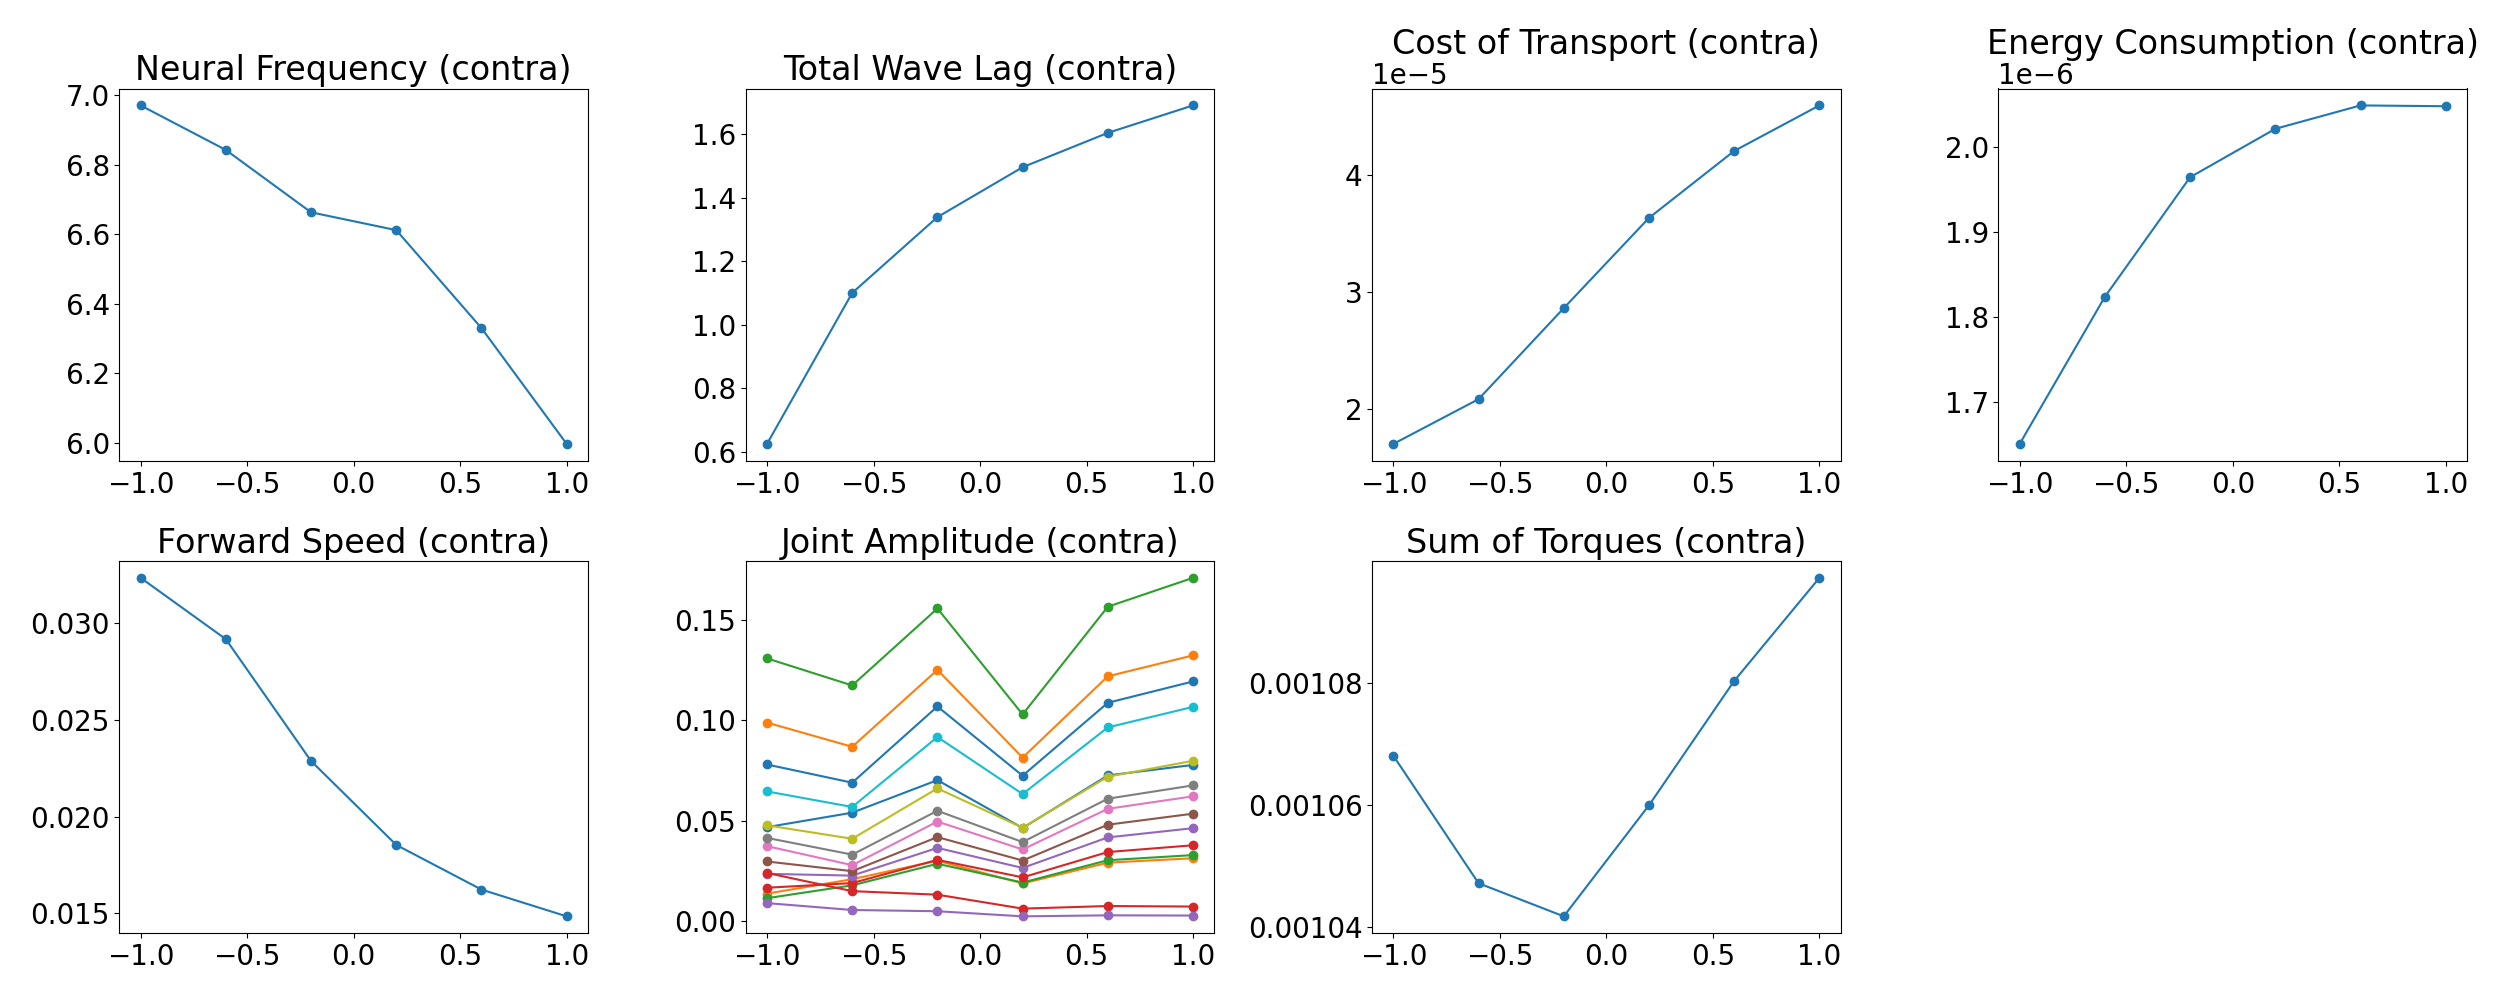
\includegraphics[width=0.8\linewidth]{our_figures/metrics_contra_variation.png}
    \caption{Controller and mechanical metrics depending on contralateral feedback strengths}
    \label{fig:metrics_contra_variation}
\end{figure}

\textbf{\underline{Question 5.5} Analyze the result qualitatively and describe the effect of ipsilateral and contralateral feedbacks on the swimming locomotion behaviors. How does it relate from the observation (at the beginning of the section) about the known sensory neurons?}.

\textbf{\underline{Answer 5.5:} }
The analysis conducted for the case where \( w^{contra} = 0 \) and \( w^{ipsi} \) is varied in the range \([-1, 1]\), scaled by \( ws\_ref \), reveals the following trends in neural and mechanical metrics. As \( w^{ipsi} \) increases, both neural frequency and forward speed also increase. This indicates that stronger positive ipsilateral feedback (excitatory) promotes more rapid neural oscillations and enhances locomotor performance, resulting in faster forward motion, while negative values (inhibitory signal) reveal an opposite trend.
Simultaneously, total wave lag, cost of transport, and energy consumption all decrease with increasing \( w^{ipsi} \). These reductions suggest that positive ipsilateral feedback improves inter-joint coordination and efficiency, likely by generating more synchronized movement patterns that require less energy and exhibit reduced temporal delays across the body segments, while negative one have an opposite influence.

Joint amplitudes across the joints remain relatively consistent over the tested range of \( w^{ipsi} \), with a subtle trend where joints with initially larger amplitudes exhibit more variation than those with smaller ones. 

The sum of torques shows a U-shaped profile: it initially decreases with slightly positive feedback but increases again at higher feedback strengths. This trend suggests that there is an optimal range of ipsilateral feedback that minimizes mechanical effort. However, even at higher values, the increase in torque remains modest, suggesting that the system can sustain improved locomotion with only a marginal rise in mechanical demands.

Overall, the results indicate that positive (excitatory) ipsilateral feedback enhances both neural control and mechanical efficiency, while maintaining stable joint actuation and avoiding excessive torque demands.

On the other hand, the analysis conducted for the case where \( w^{ipsi} = 0 \) and \( w^{contra} \) is varied in the range \([-1, 1]\), scaled by \( ws\_ref \), reveals opposite trends in neural and mechanical metrics. 

\begin{comment}

In this configuration, neural frequency and forward speed both tend to decrease as \( w^{contra} \) increases. This suggests that stronger positive contralateral feedback has a dampening effect on the locomotor rhythm, leading to slower oscillations and reduced propulsive performance.


Conversely, total wave lag, cost of transport, and energy consumption all increase with increasing \( w^{contra} \). These results indicate a decline in inter-joint coordination and locomotor efficiency, implying that excessive ipsilateral feedback may disrupt the timing relationships between limbs, causing less synchronized and more energetically costly movement.

Joint amplitudes show a slight upward trend, particularly among joints with initially higher amplitudes, suggesting that the system compensates for reduced neural drive and coordination by increasing the range of limb motion. This could reflect an attempt to maintain effective locomotion under less efficient control conditions.

The sum of torques also exhibits a slight increase with positive contralateral feedback, indicating that greater mechanical effort is required to maintain movement as coordination deteriorates. This additional torque demand, coupled with higher energy consumption, underscores the destabilizing effect of excessive contralateral feedback on the motor system.
\end{comment}

These findings highlight a contrast between the roles of contralateral and ipsilateral feedback: while positive ipsilateral feedback (excitatory) enhances both neural and mechanical performance, excessive positive contralateral lateral feedback (excitatory) appears to hinder coordination, reduce efficiency, and increase the mechanical burden of locomotion. These results are aligned with the theory of sensory feedback, where to have an efficient swimming motion it is important to have excitatory ipsilateral signal and inhibitory contralateral signals from proprioceptive sensory neurons. These results can also be interpreted in terms of feedback regulation of stretch: positive ipsilateral and negative contralateral feedback together form an effective negative feedback loop, counteracting stretch and promoting stability. In contrast, reversing the sign of either feedback transforms the system into a positive feedback loop, which amplifies stretch and may destabilize the motion pattern—until intrinsic rhythm-generating mechanisms such as central pattern generators (CPGs) reassert control.


\subsection*{6. Swimming under perturbations}

In the lamprey it has been shown that an external rhythmic bending, imposed during the activation of the CPG network, has the capability to modulate the frequency of the ongoing oscillations so that they synchronize with the external stimulus. This synchronization is made possible by the proprioceptive sensory neurons and their direct connections to the CPG segments.

In this exercise, we test the stability of the closed-loop CPG controller under external perturbations. Specifically, we apply a rhythmic bending (entrainment) of 45 degrees with a fixed frequency on the axial joints. The implementation of the rhythmic bending is already provided in a helper function \fileref{define\_entraining\_signals} (check \fileref{util/entraining\_signals.py} for detailed implementations and you need to pass the output of entraining\_signals in the SimulationParameters class to access the prescribed kinematics given by entraining\_signals in network\_ode).

Hint: Since we're imposing a movement on the zebrafish, the joint positions are already known and we don't need to do a full physical simulation.
If you still want to visualize the swimming behavior, import \fileref{run\_single} from \fileref{util.run\_closed\_loop} instead of \fileref{util.run\_open\_loop}.

\textbf{\underline{Question 6.1} Explore the entrainment by running \fileref{exercise7.py}, where a default entrainment of 45 degrees at 8 Hz is implemented. Report the neural frequency of the controller. How does the frequency compare to the simulation without entrainment? Does this match your expectation and why?}

\textbf{\underline{Answer 6.1}}

As with the previous exercise, we ran the simulations with the pre-set initial phases, that is a gradient of phases from 0 to $2\pi$ rostro-caudally.
The neural frequency of the entrained controller is 6.66 Hz, while the reference, non entrained neural frequency is 6.66 Hz. We would expect an increase in frequency since the entraining signal at 8 Hz is faster than the reference neural frequency. The absence of this syncronization is the result of a weak coupling ($w$) between the entraining signals and the controller, which was set at $w^{ipsi}=-w^{contra}=0.25*w s_{ref}$.

\textbf{\underline{Question 6.2} Explore the effect of the entrainment on the neural frequency under different feedback gain strengths systematically in \fileref{exercise8.py}. For simplicity, we take $w^{ipsi} = -w^{contra} = w$
Specifically, run the simulation with feedback gains $w$ in range [0,2] scaled by $ws\_ref$ and entrainment frequencies in range [3.5,10] in a 2D grid. Take $w=0$ (no feedback) as a reference baseline with reference neural frequency. Plot the difference between the entrainment frequency and the reference frequency vs. the difference between the actual resulting neural frequency and the reference frequency. Describe and qualitatively analyze your observations.}


\textbf{\underline{Answer 6.2}}

In Figure \ref{fig:exercise62} we can see the effect of the coupling weight and the difference ($\Delta f = f^{entr} - f^{ref}$) between the entraining frequency ($f^{entr}$) and the reference frequency ($f^{ref}$), on the actual neural frequency ($f$). The x-axis is $\Delta f$, while the y-axis is $f-f^{ref}$.

As a trend, we observe that as $|\Delta f|$ increases, $f$ tends to follow in a phase-locked fashion with a lag on the actual frequency, until a threshold beyond which synchronization begins to fail. This breaking point extends further as the coupling weight $w$ increases, as illustrated in both Figure \ref{fig:exercise62a} and Figure \ref{fig:exercise62b}, highlighting the Arnold tongue nature of synchronization.


With an increase of $w$, we can also see a decrease in the frequency lag $f-f^{entr}$, which in the graphs $f-f^{ref}\,vs\,\Delta f$ corresponds to a slope approaching one.

\begin{figure}[H]
  \centering
  \begin{minipage}{0.48\textwidth}
    \centering
    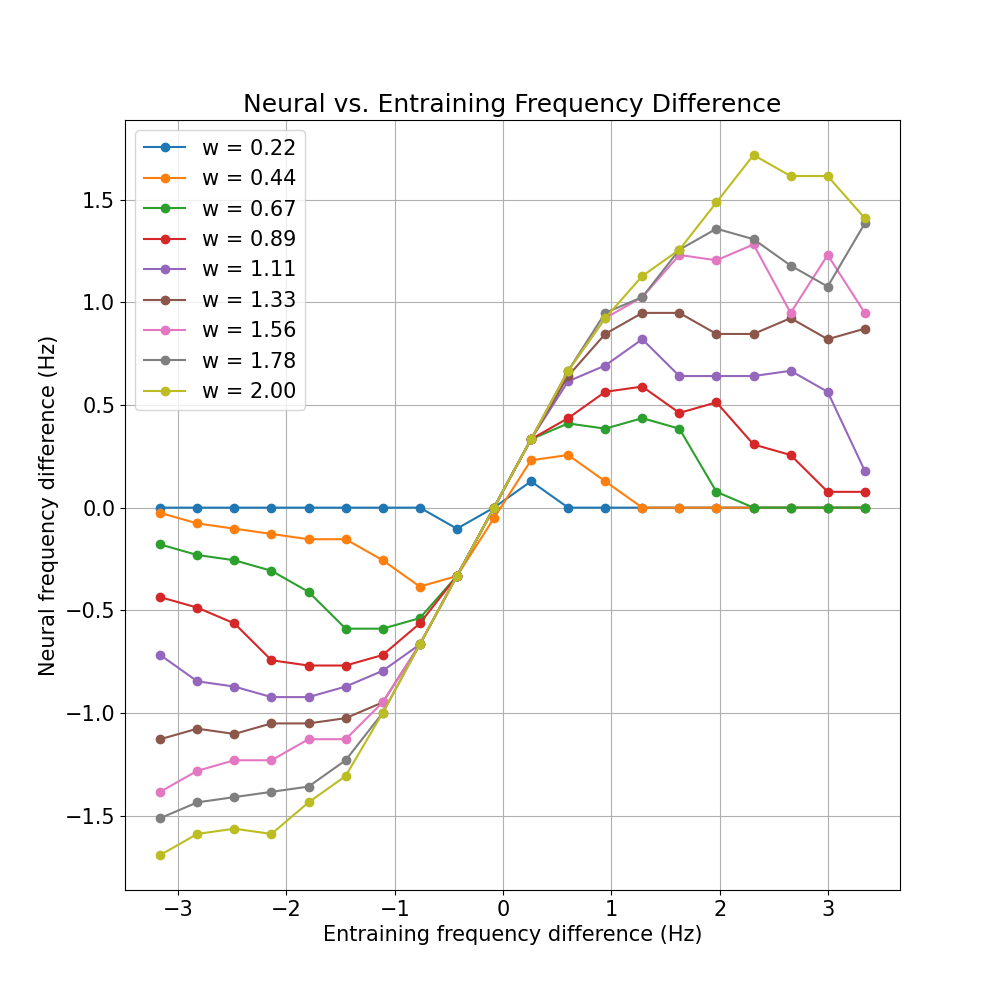
\includegraphics[width=\linewidth]{our_figures/exercise8_frequency_diff.png}
    \subcaption{Increasing $w$ allows broader $\Delta f$ before desynchronization.}
    \label{fig:exercise62a}
  \end{minipage}
  \hfill
  \begin{minipage}{0.48\textwidth}
    \centering
    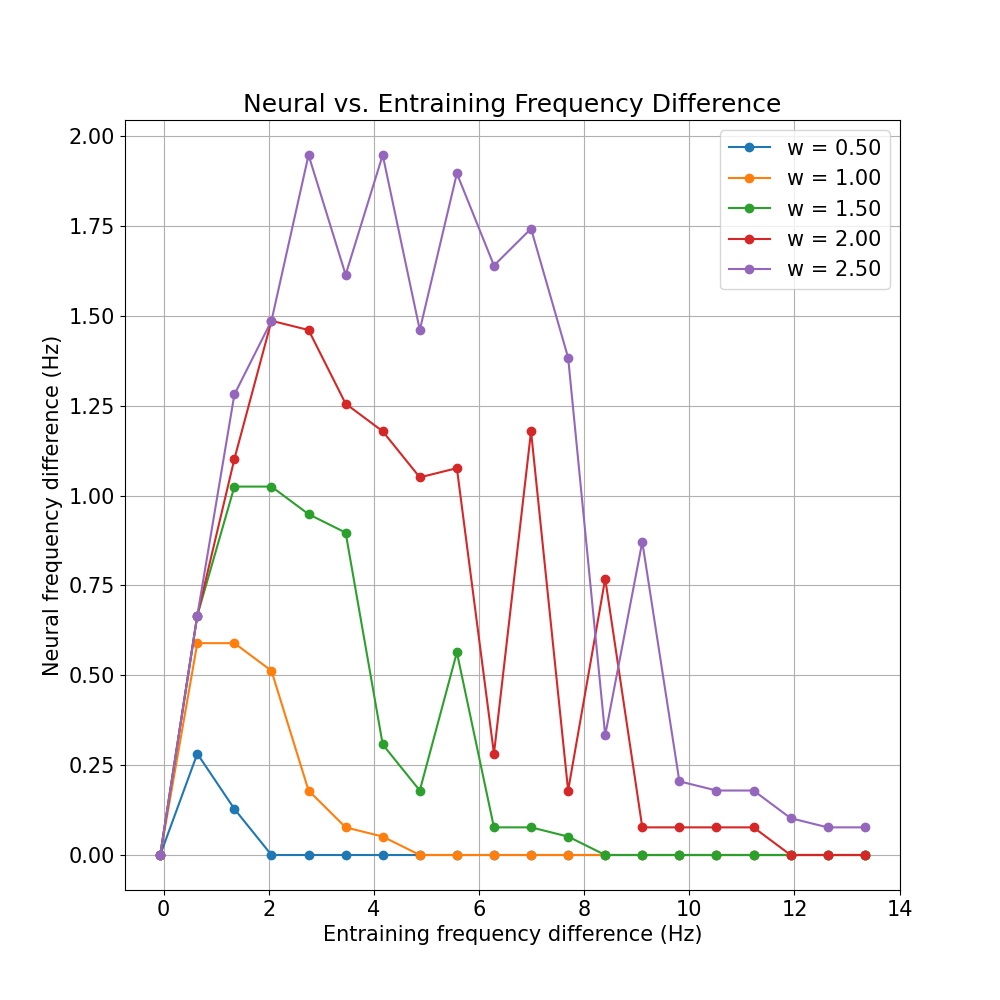
\includegraphics[width=\linewidth]{our_figures/exercise8bis_frequency_diff.png}
    \subcaption{Even for high $w$, large $\Delta f$ leads to desynchronization.}
    \label{fig:exercise62b}
  \end{minipage}
  \caption{Effect of coupling weight and entraining frequency on neural synchronization. (a) shows improved synchronization with increased $w$. (b) shows desynchronization for excessive $\Delta f$ despite high $w$.}
  \label{fig:exercise62}
\end{figure}

This effect is more clearly illustrated in the entrainment map shown in Figure \ref{fig:arnold_tongue}. The plot displays the difference between the actual neural frequency and the entraining frequency as a function of the coupling gain $w$ and the entraining frequency. The red regions indicate conditions under which the oscillator was successfully entrained.

The degree of entrainment is quantified by a fitness function, defined as:
\[
\textbf{Fitness} =  \frac{4}{\pi}\arctan\left(\frac{f-f^{\text{ref}}}{f^{\text{entr}}-f^{\text{ref}}}\right)
\]

This function takes values close to 1 when the actual frequency $f$ closely matches the entraining frequency $f^{\text{entr}}$, and approaches 0 when $f$ remains at the reference (unperturbed) frequency $f^{ref}$, indicating no entrainment.
\begin{figure}[H]
    \centering
    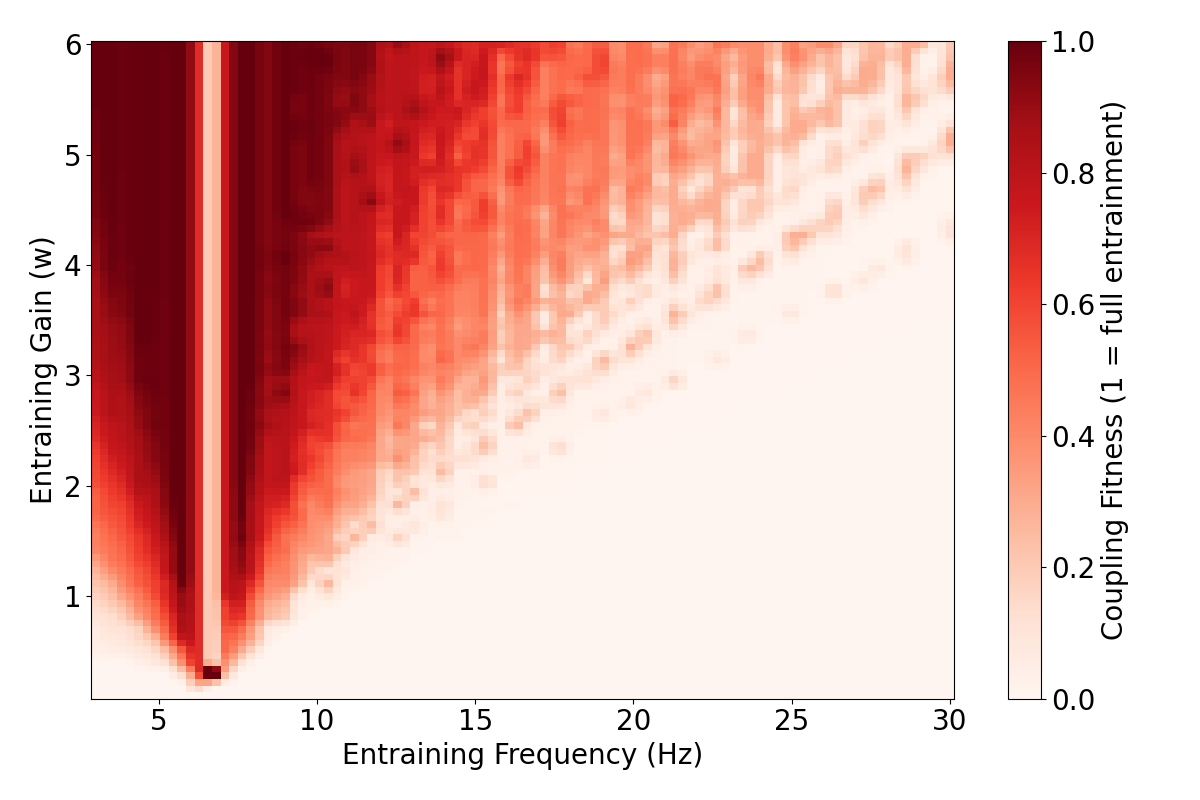
\includegraphics[width=0.8\linewidth]{our_figures/exercise8_arnold_tongue_fitness_interpolated.png}
    \caption{Entrainment of the controller as a function of entraining frequency and coupling gain $w$}
    \label{fig:arnold_tongue}
\end{figure}

An artifact appears around the reference neural frequency of approximately 6.66 Hz, where the entraining signal matches the natural frequency of the system. In this region, the fitness drops artificially to zero because the denominator of the fitness function becomes very small, which is indistinguishable from a lack of entrainment. Additionally, some of the shading irregularities in the map arise from the interpolation method used in plotting.

At higher coupling strengths and entraining frequencies, the Arnold tongue becomes less smooth and displays local peaks and valleys. These features arise likely from non linear entrainment at higher order ratios (harmonic and subharmonic), such as 2:1, 3:1, or 3:2, also visible in Figure \ref{fig:exercise62b} at high coupling values. 
\begin{comment}At entraining frequency at ratios of 2:1 and 3:1 with the reference frequency, corresponding to frequencies of around 13 and 19 Hz, we see the system less entrained, since the entrainment signal goes faster but matches the system's phase every two or three cycles.\end{comment}

\subsection*{7. CPG-free swimming with proprioceptive feedback}

In last parts of the project we implemented an open-loop CPG and a closed-loop CPG with sensory feedback. Now we want to study if the local proprioceptive feedback alone is enough to elicit the swimming behavior.

\textbf{\underline{Question 7.1} Try removing the ipsilateral connection from the CPG model while preserving the stretch feedback in \fileref{exercise9.py}. Test if the fish could still initiate the swimming behavior. Does the result change if you alter the feedback strengths? Summarize and explain your observations and use plots/videos if needed.}

\textit{\underline{Answer 7.1}}

In Figure 12, we see that swimming isn’t hindered for any impairment type when the CPG phases are initialized with the default values. The only noticeable difference is a slightly higher oscillation amplitude with ipsilateral inhibition, nothing else. In contrast, when phases are initialized randomly, as in Figures 13 and 14, the effects of impairments become much more visible. This suggests that feedback alone is enough to maintain an already stabilized gait but might not be sufficient to initiate one. To properly test whether gait can be initialized despite impairments, phases need to be initialized randomly.

Looking at the swimming behavior in Figure 13 with no impairment, the fish swims well and travels slightly further as feedback strength increases. Although, beyond w=2, there is little improvement in performance. When ipsilateral connections are removed, the fish still manages to swim, but it doesn’t go as far. In this case, feedback strength has a much stronger effect: with w=0.5, the fish travels less than one-fifth of the original (unimpaired) distance, while at w=2, it reaches over two-thirds of that distance. Interestingly, without ipsilateral connections, the oscillation amplitudes are higher, which might explain the drop in swimming efficiency. This shows that the fish can still swim without ipsilateral connections in the CPG, meaning their role is limited. They might mainly serve to keep oscillation amplitudes in a certain range by reducing them, rather than being essential to initiate gait, assuming that there is a strong enough feedback. This also confirms what we saw in Part 5, feedback is important for effective locomotion.

\begin{figure}[htbp]
  \centering
  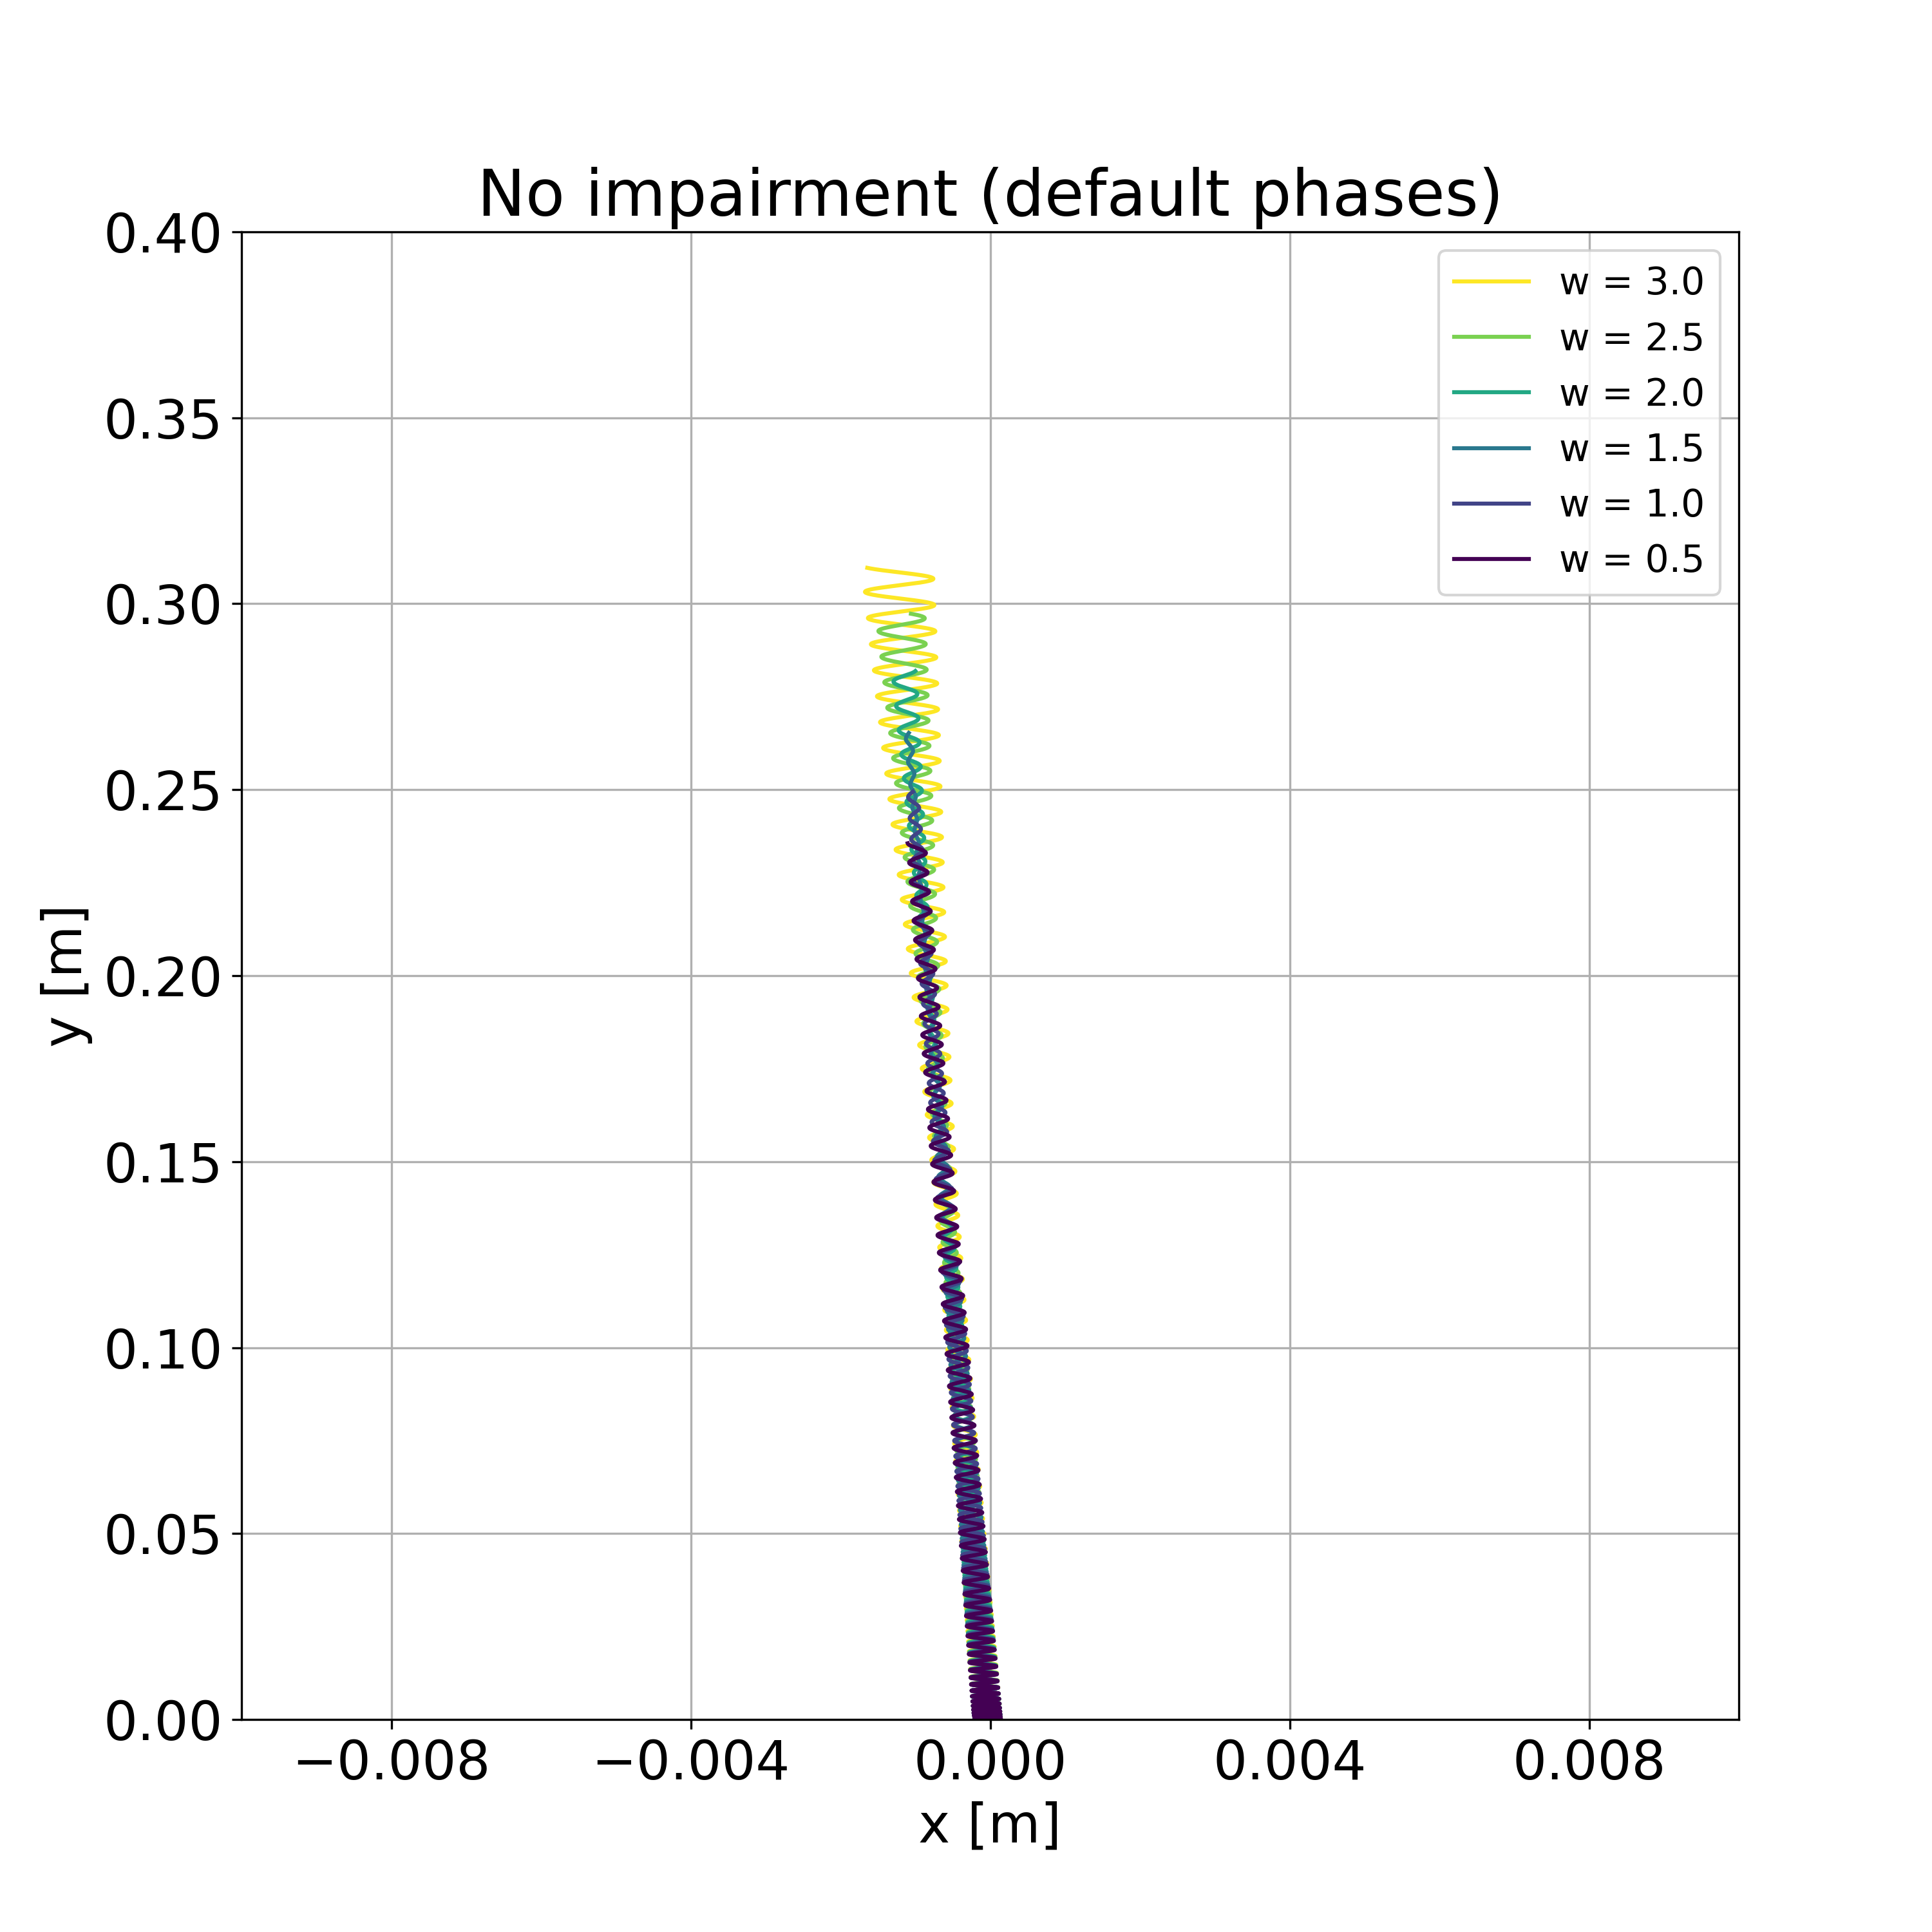
\includegraphics[width=0.23\textwidth]{our_figures/No impairment_default.png}
  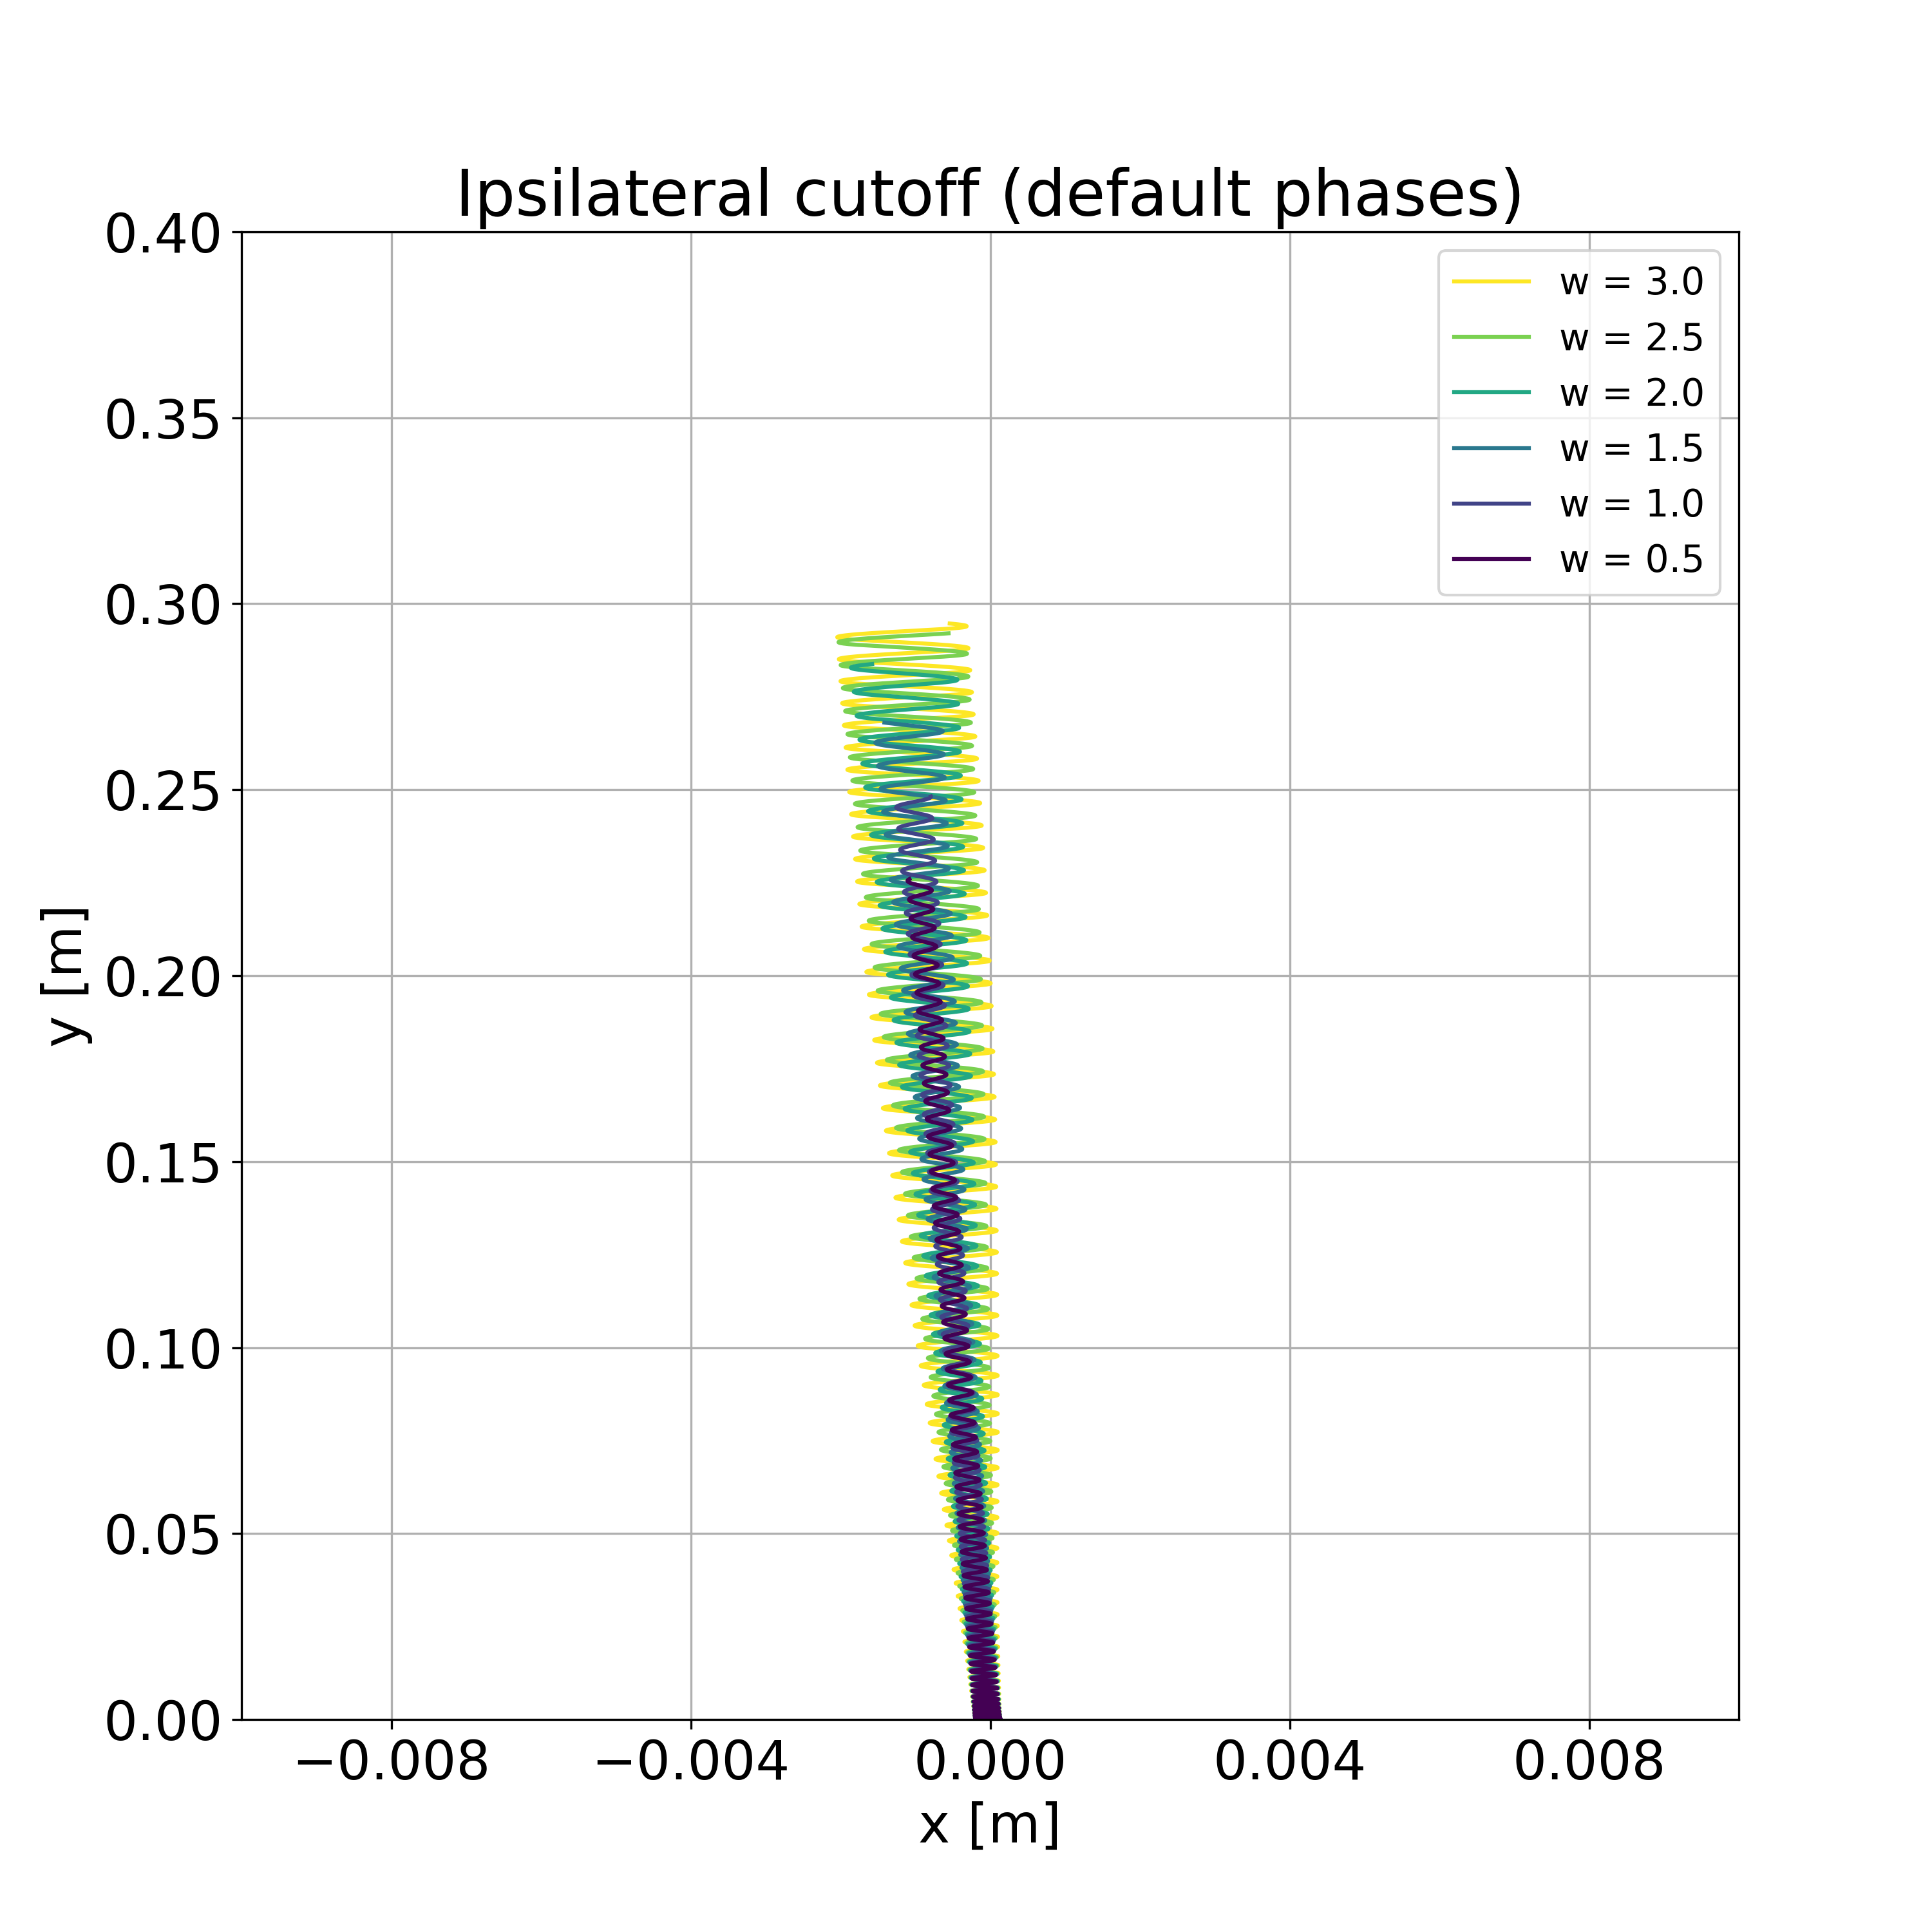
\includegraphics[width=0.23\textwidth]{our_figures/Ipsilateral cutoff_default.png}
  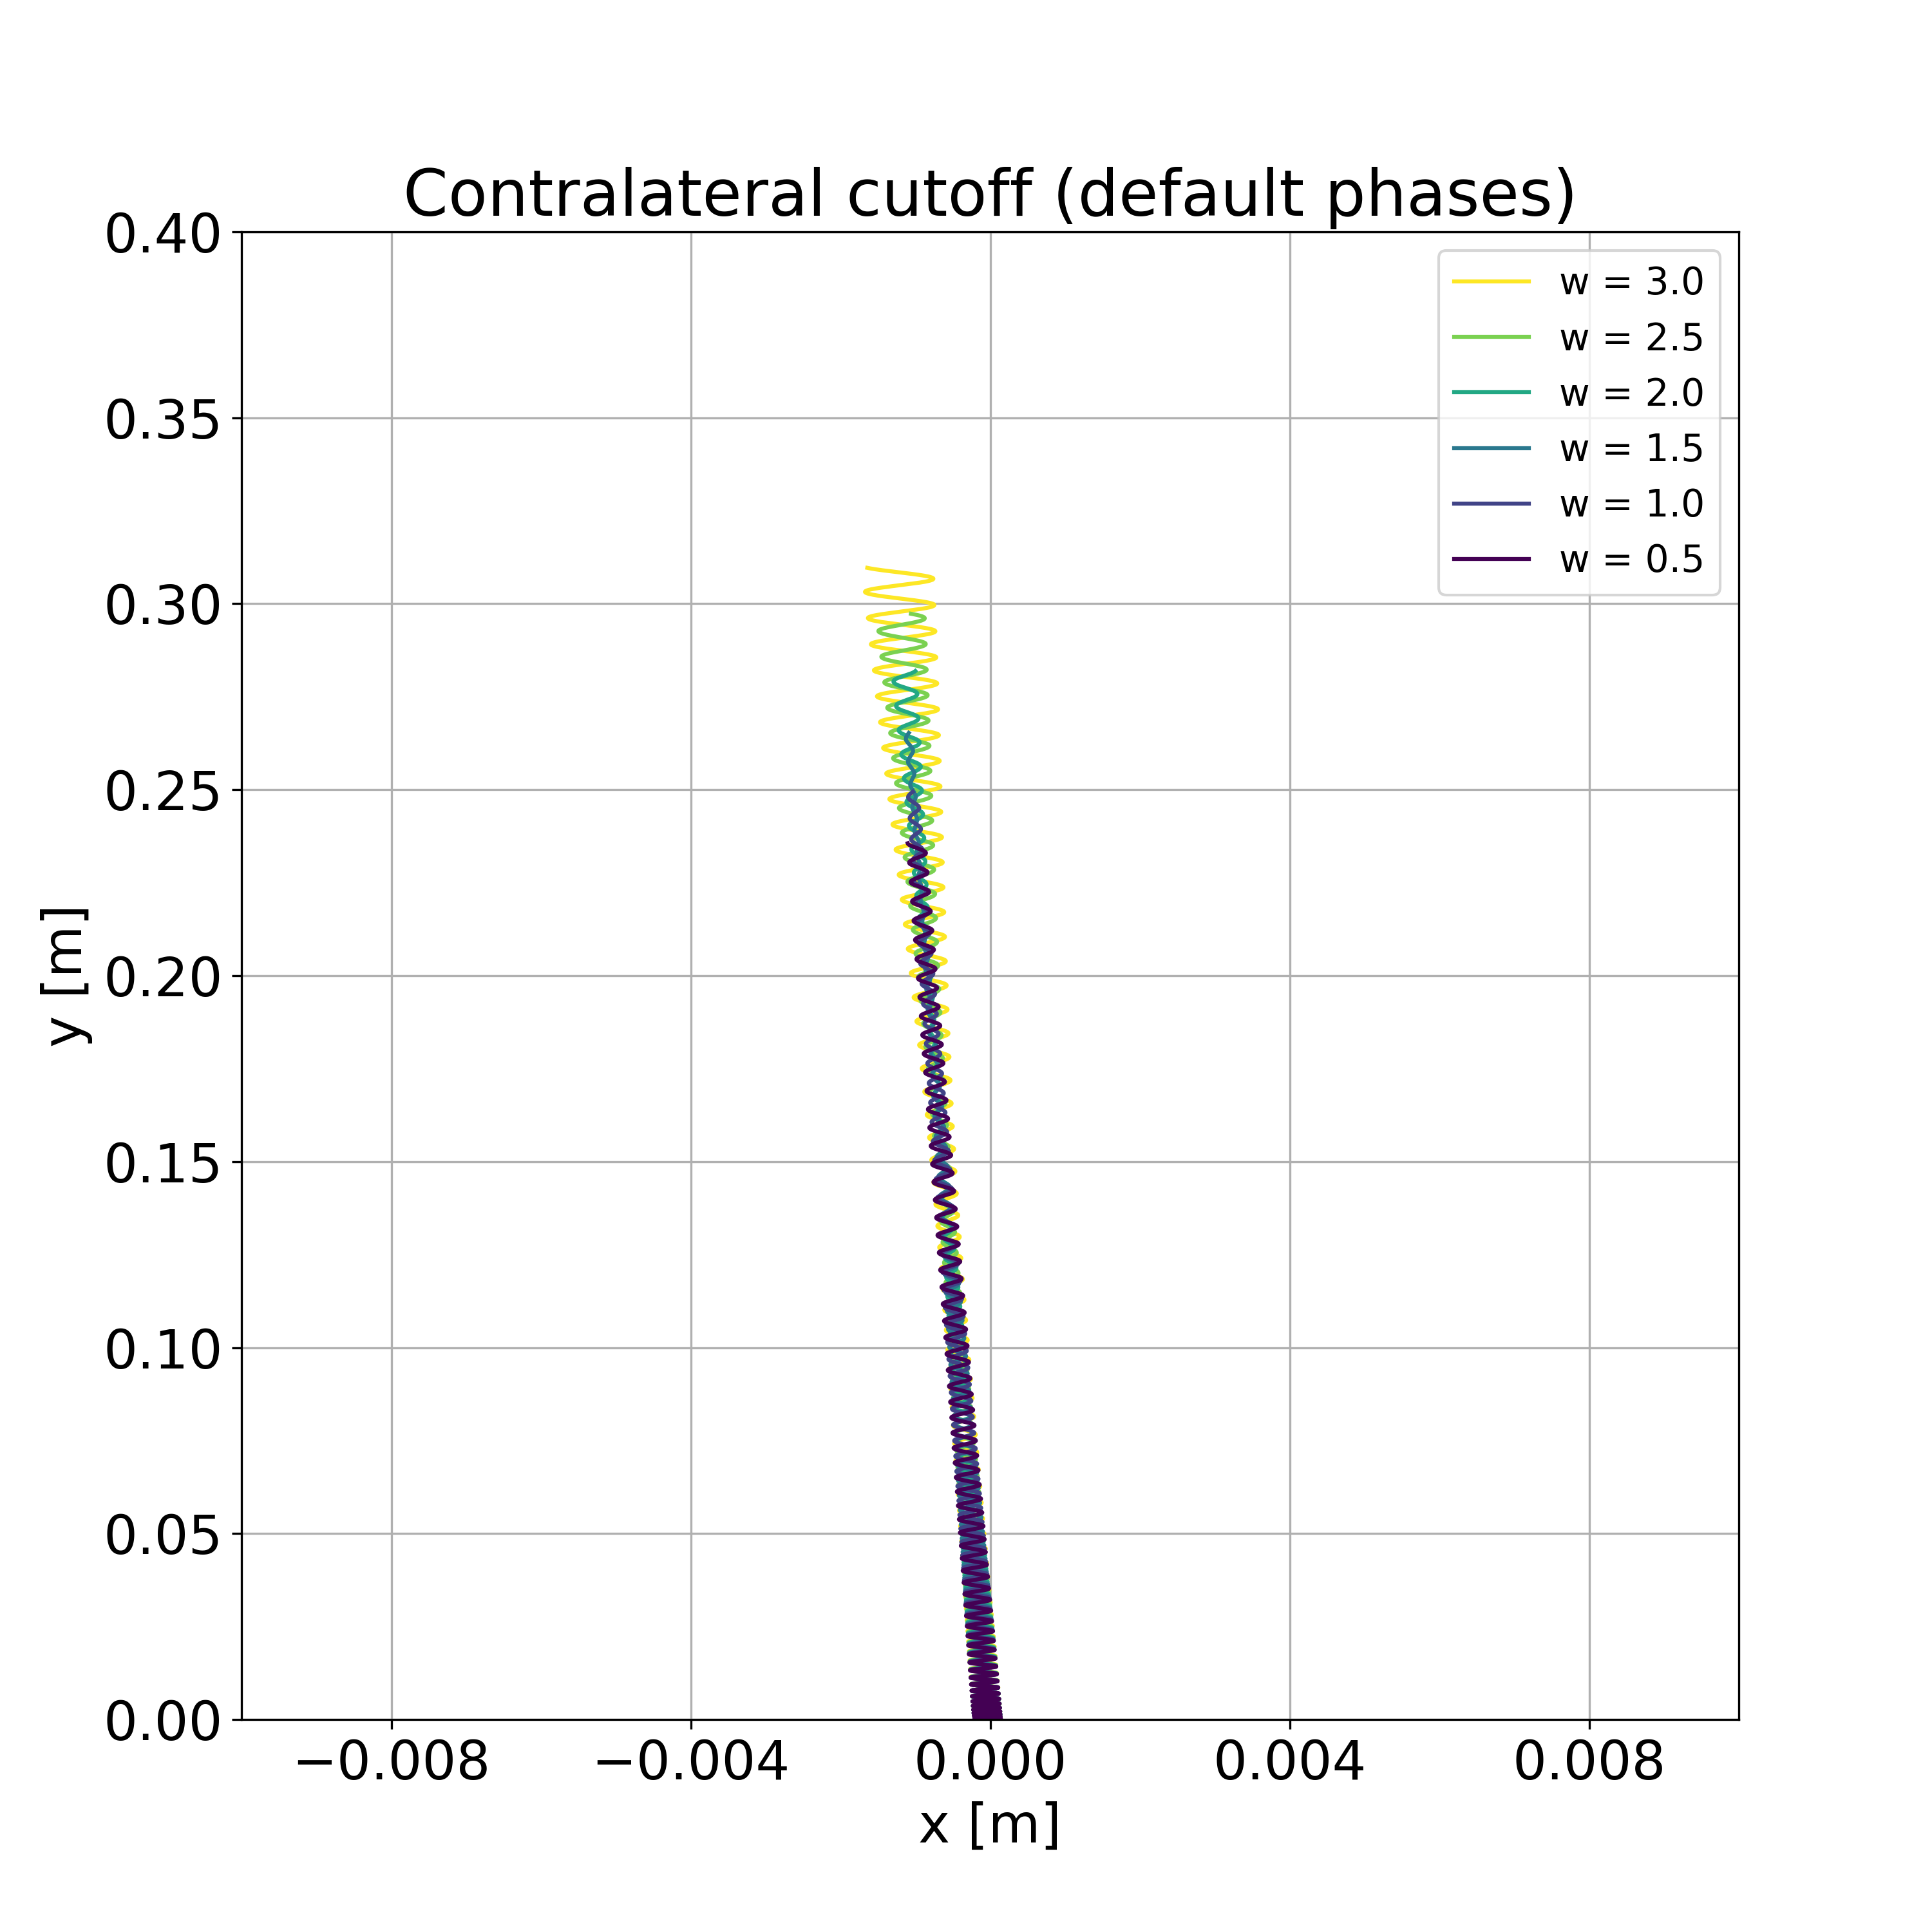
\includegraphics[width=0.23\textwidth]{our_figures/Contralateral cutoff_default.png}
  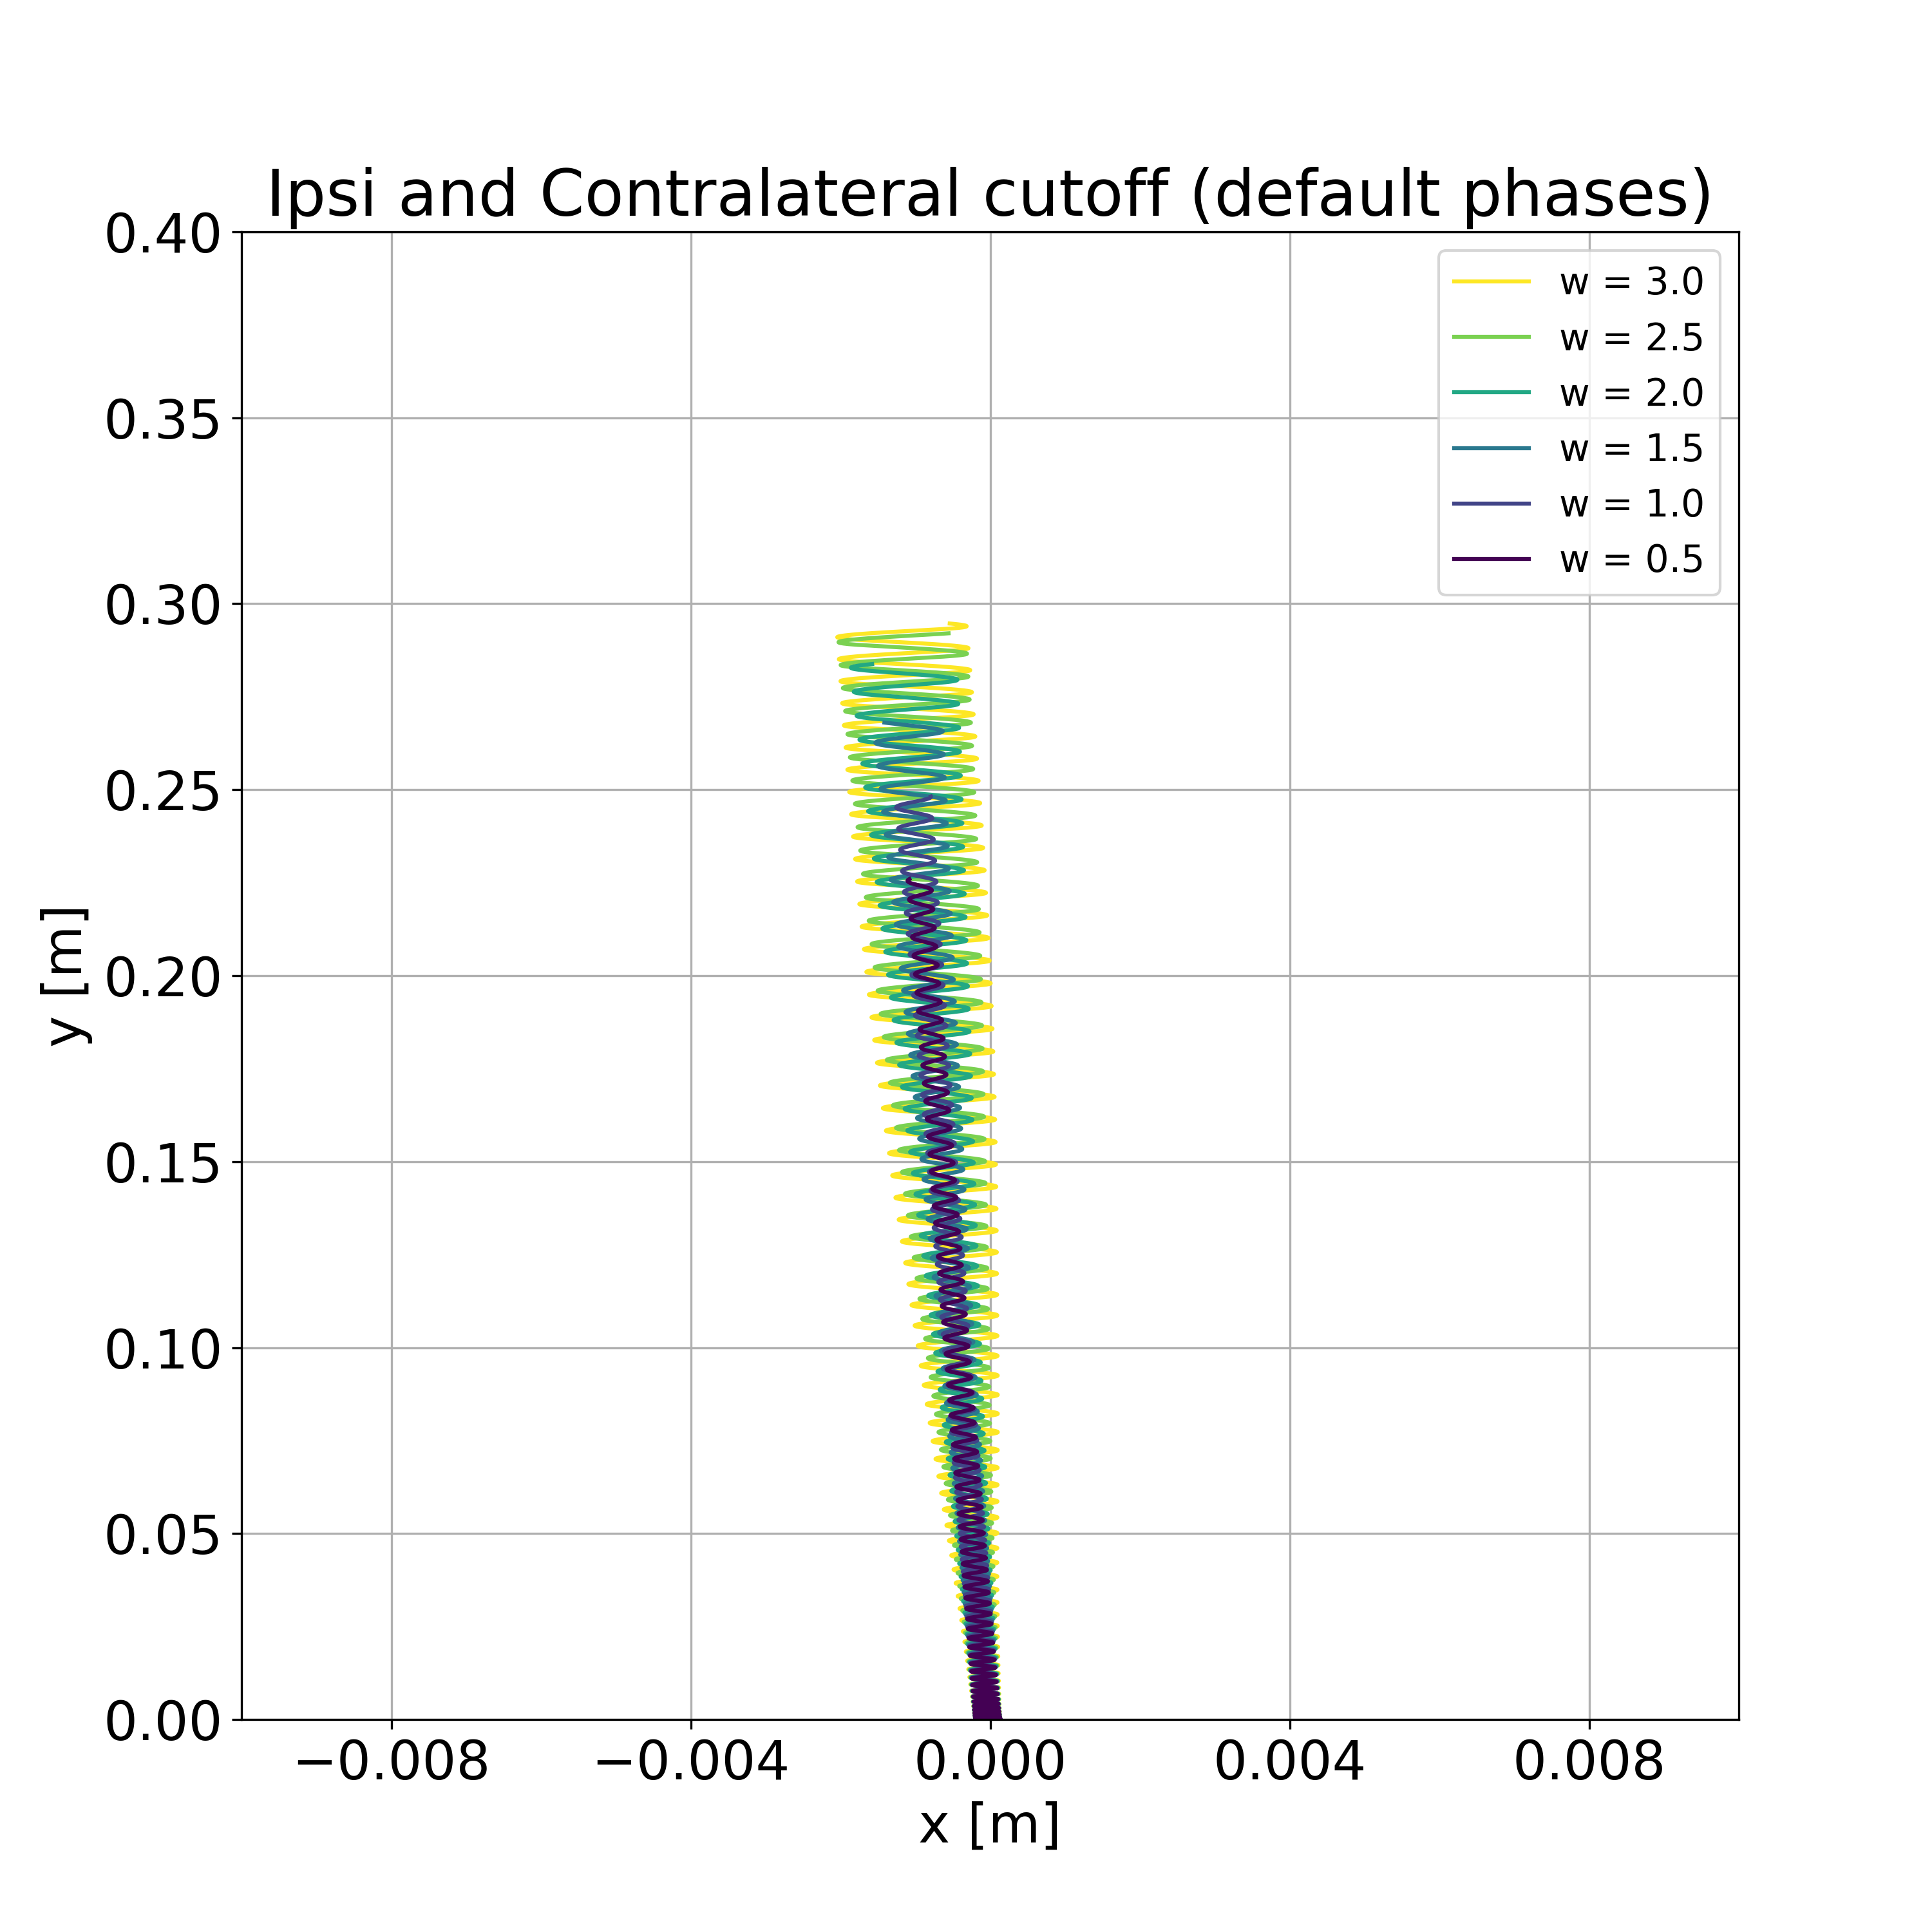
\includegraphics[width=0.23\textwidth]{our_figures/Ipsi and Contralateral cutoff_default.png}
  \caption{All Impairment types with default phases.}
  \label{fig:default_phases}
\end{figure}

\begin{figure}[H]
    \centering
    \begin{subfigure}[t]{0.48\linewidth}
        \centering
        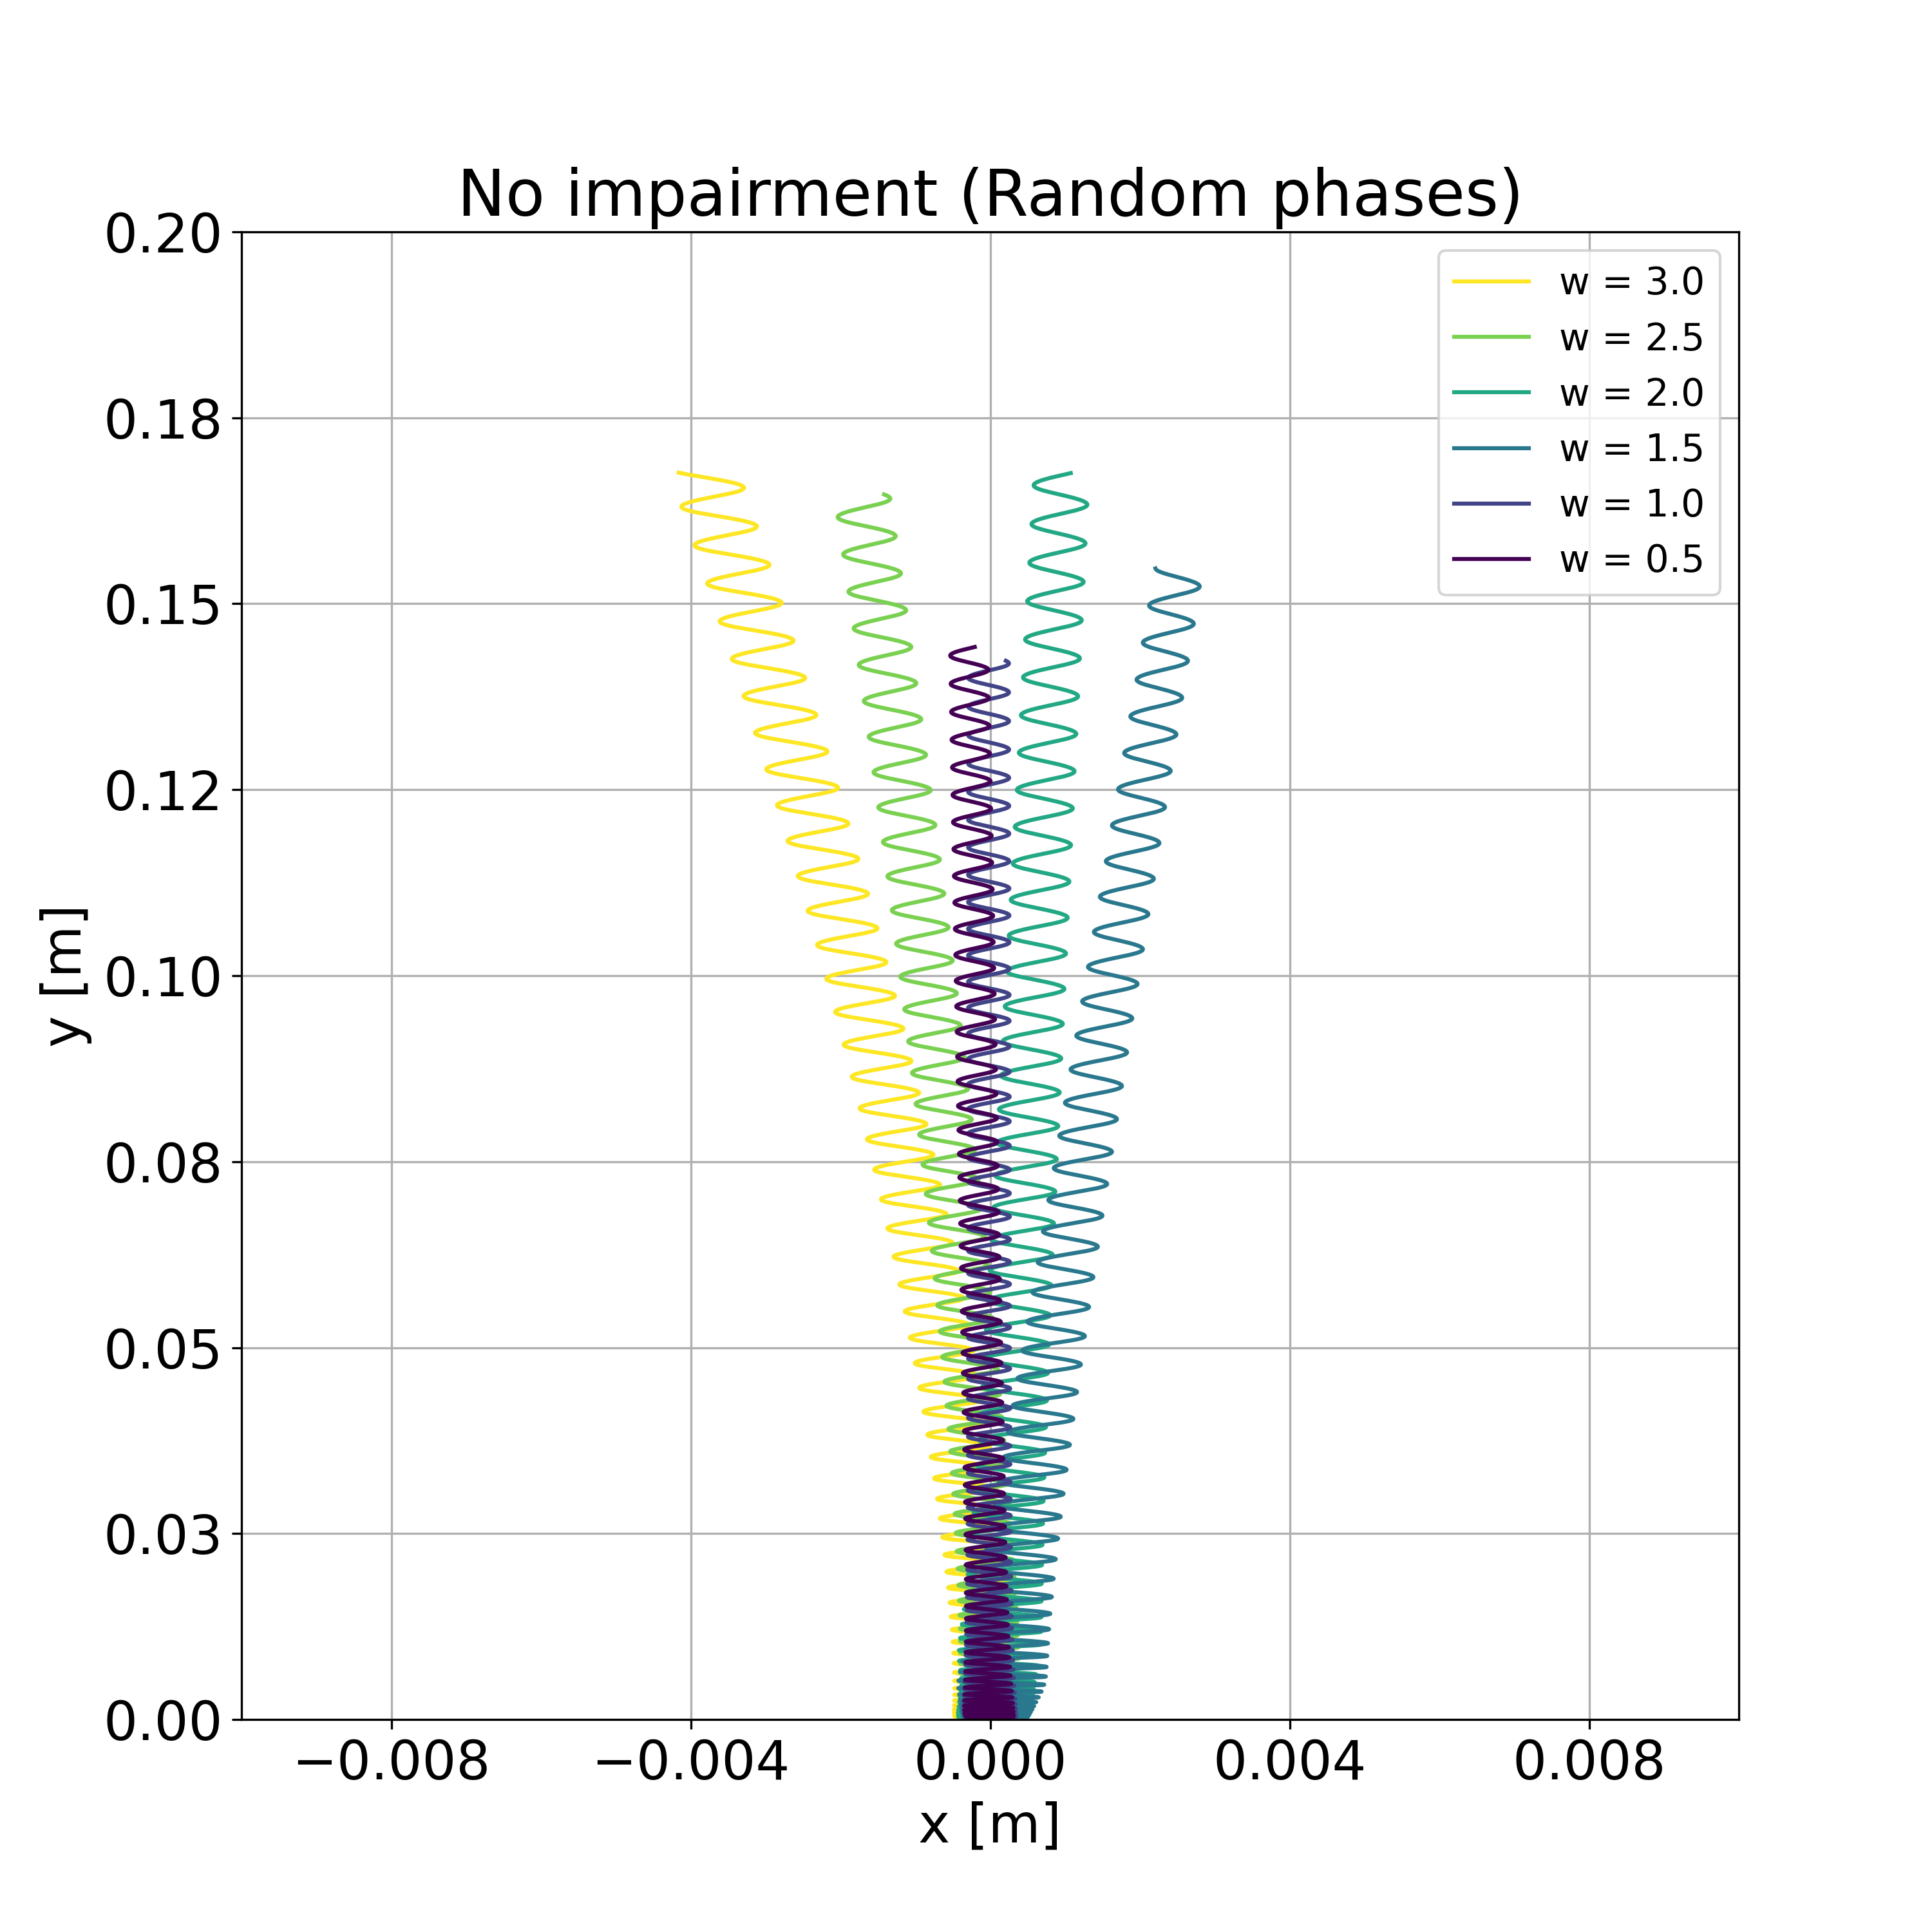
\includegraphics[width=\linewidth]{our_figures/No impairment_random.png}
        \caption{Trajectory of the fish's head without impairment for different feedback gain $w$.}
        \label{fig:no_impairment_random}
    \end{subfigure}
    \hfill
    \begin{subfigure}[t]{0.48\linewidth}
        \centering
        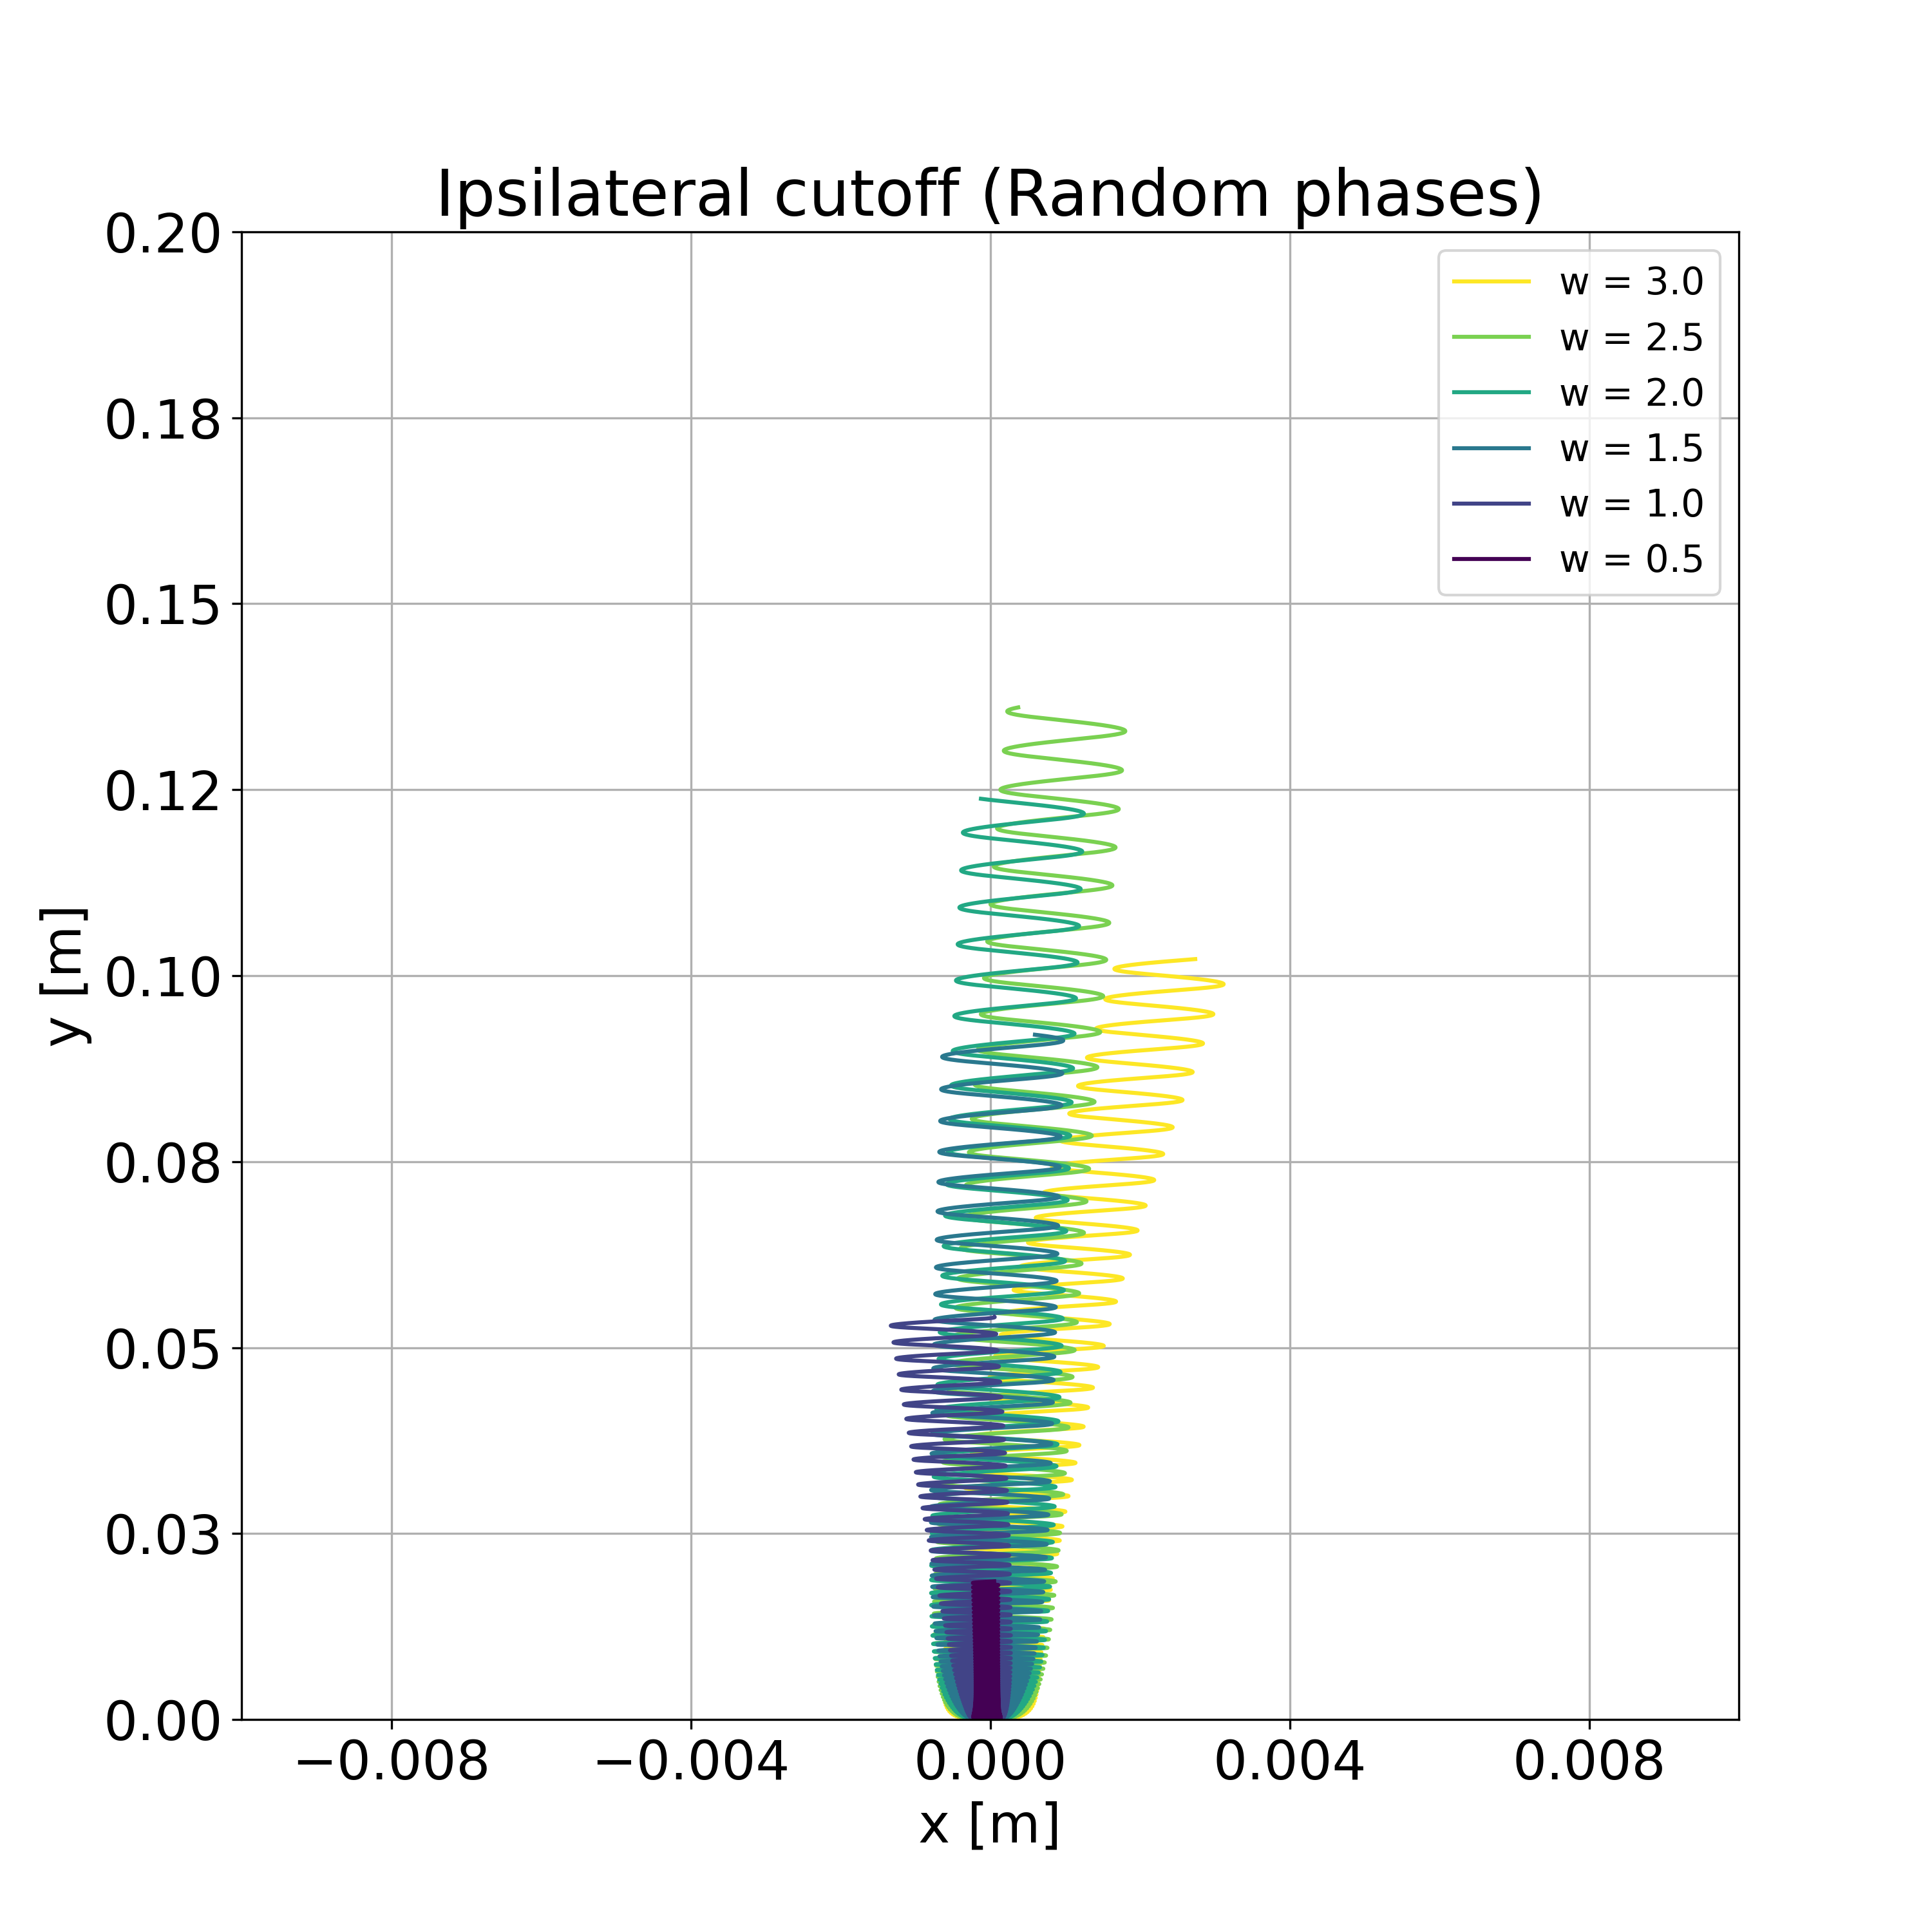
\includegraphics[width=\linewidth]{our_figures/Ipsilateral cutoff_random.png}
        \caption{Trajectory of the fish's head under ipsilateral cutoff for different feedback gain $w$.}
        \label{fig:ipsi_cutoff_random}
    \end{subfigure}
    \caption{Comparison of fish head trajectories with and without ipsilateral impairment (random initial phases).}
    
\end{figure}

\textbf{\underline{Question 7.2} Repeat the experiments and try removing the contralateral connections or both ipsilateral and contralateral connections. Can you still generate the swimming behavior? If yes, report the feedback parameters used, record a video, and analyze how the CPG-free swimming compares to CPG swimming. If not, analyze the minimum CPG connections needed to elicit a swimming behavior.
}

\textit{\underline{Answer 7.2}}

Comparing Figure 13a and Figure 14, contralateral cutoff completely hinders swimming behavior. Strangely, with lower feedback, the fish goes a bit farther, but the trajectory is heavily shifted to the left. Other simulations showed a shift to the right instead, this depends on the randomly initialized phases, but some kind of side deviation is always there, with very little forward movement. When both ipsilateral and contralateral connections are cut, the result is even worse as the fish barely moves at all.

Also, unlike ipsilateral connections, contralateral ones seem important for generating higher oscillation amplitudes, as with contralateral cutoff, the oscillations are really slim. This shows that contralateral connections are important to stabilize gait and keep amplitude high, but also to initialize the gait in the first place, as it seems to control the generation of higher amplitude. Thus, feedback alone isn't enough to generate swimming if the contralateral connections are missing. Now the question that remains is: how much contralateral strength is actually needed to properly initialize the gait?

\begin{figure}[H]
    \centering
    \begin{subfigure}[t]{0.48\linewidth}
        \centering
        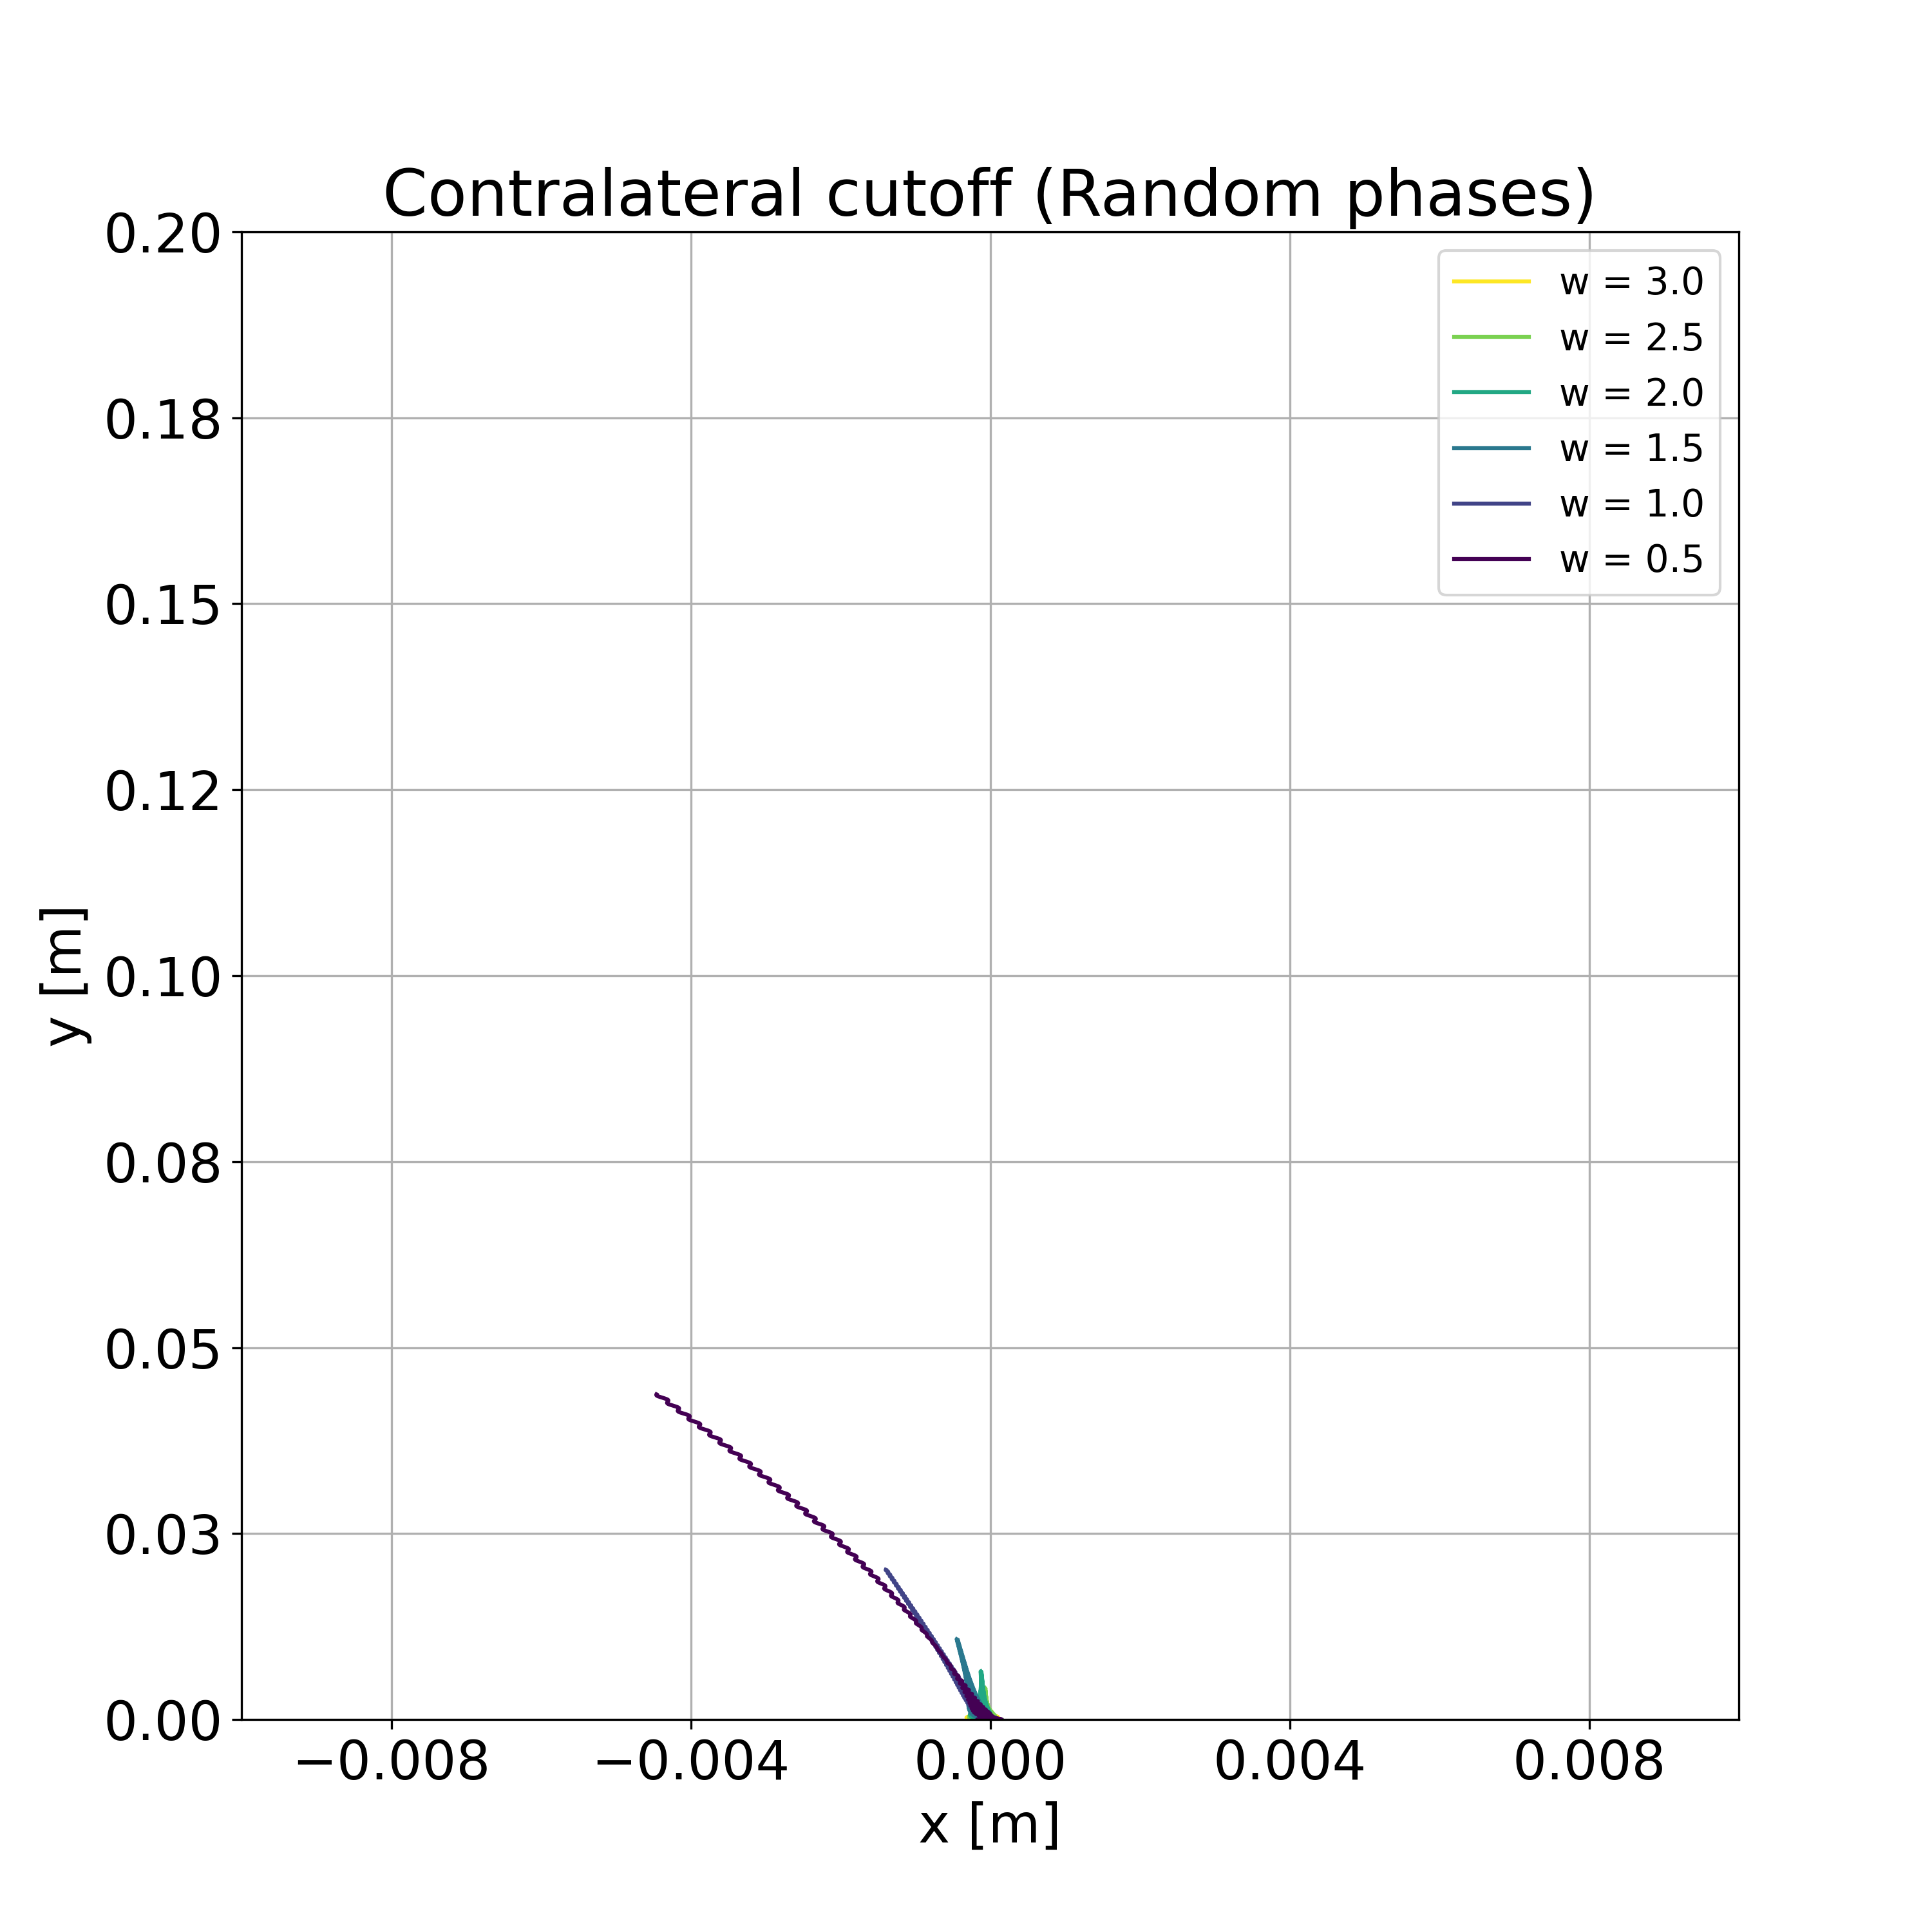
\includegraphics[width=\linewidth]{our_figures/Contralateral cutoff_random.png}
        \caption{Trajectory of the fish's head under contralateral impairment for different feedback gain $w$.}
        \label{fig:contra_cutoff_random}
    \end{subfigure}
    \hfill
    \begin{subfigure}[t]{0.48\linewidth}
        \centering
        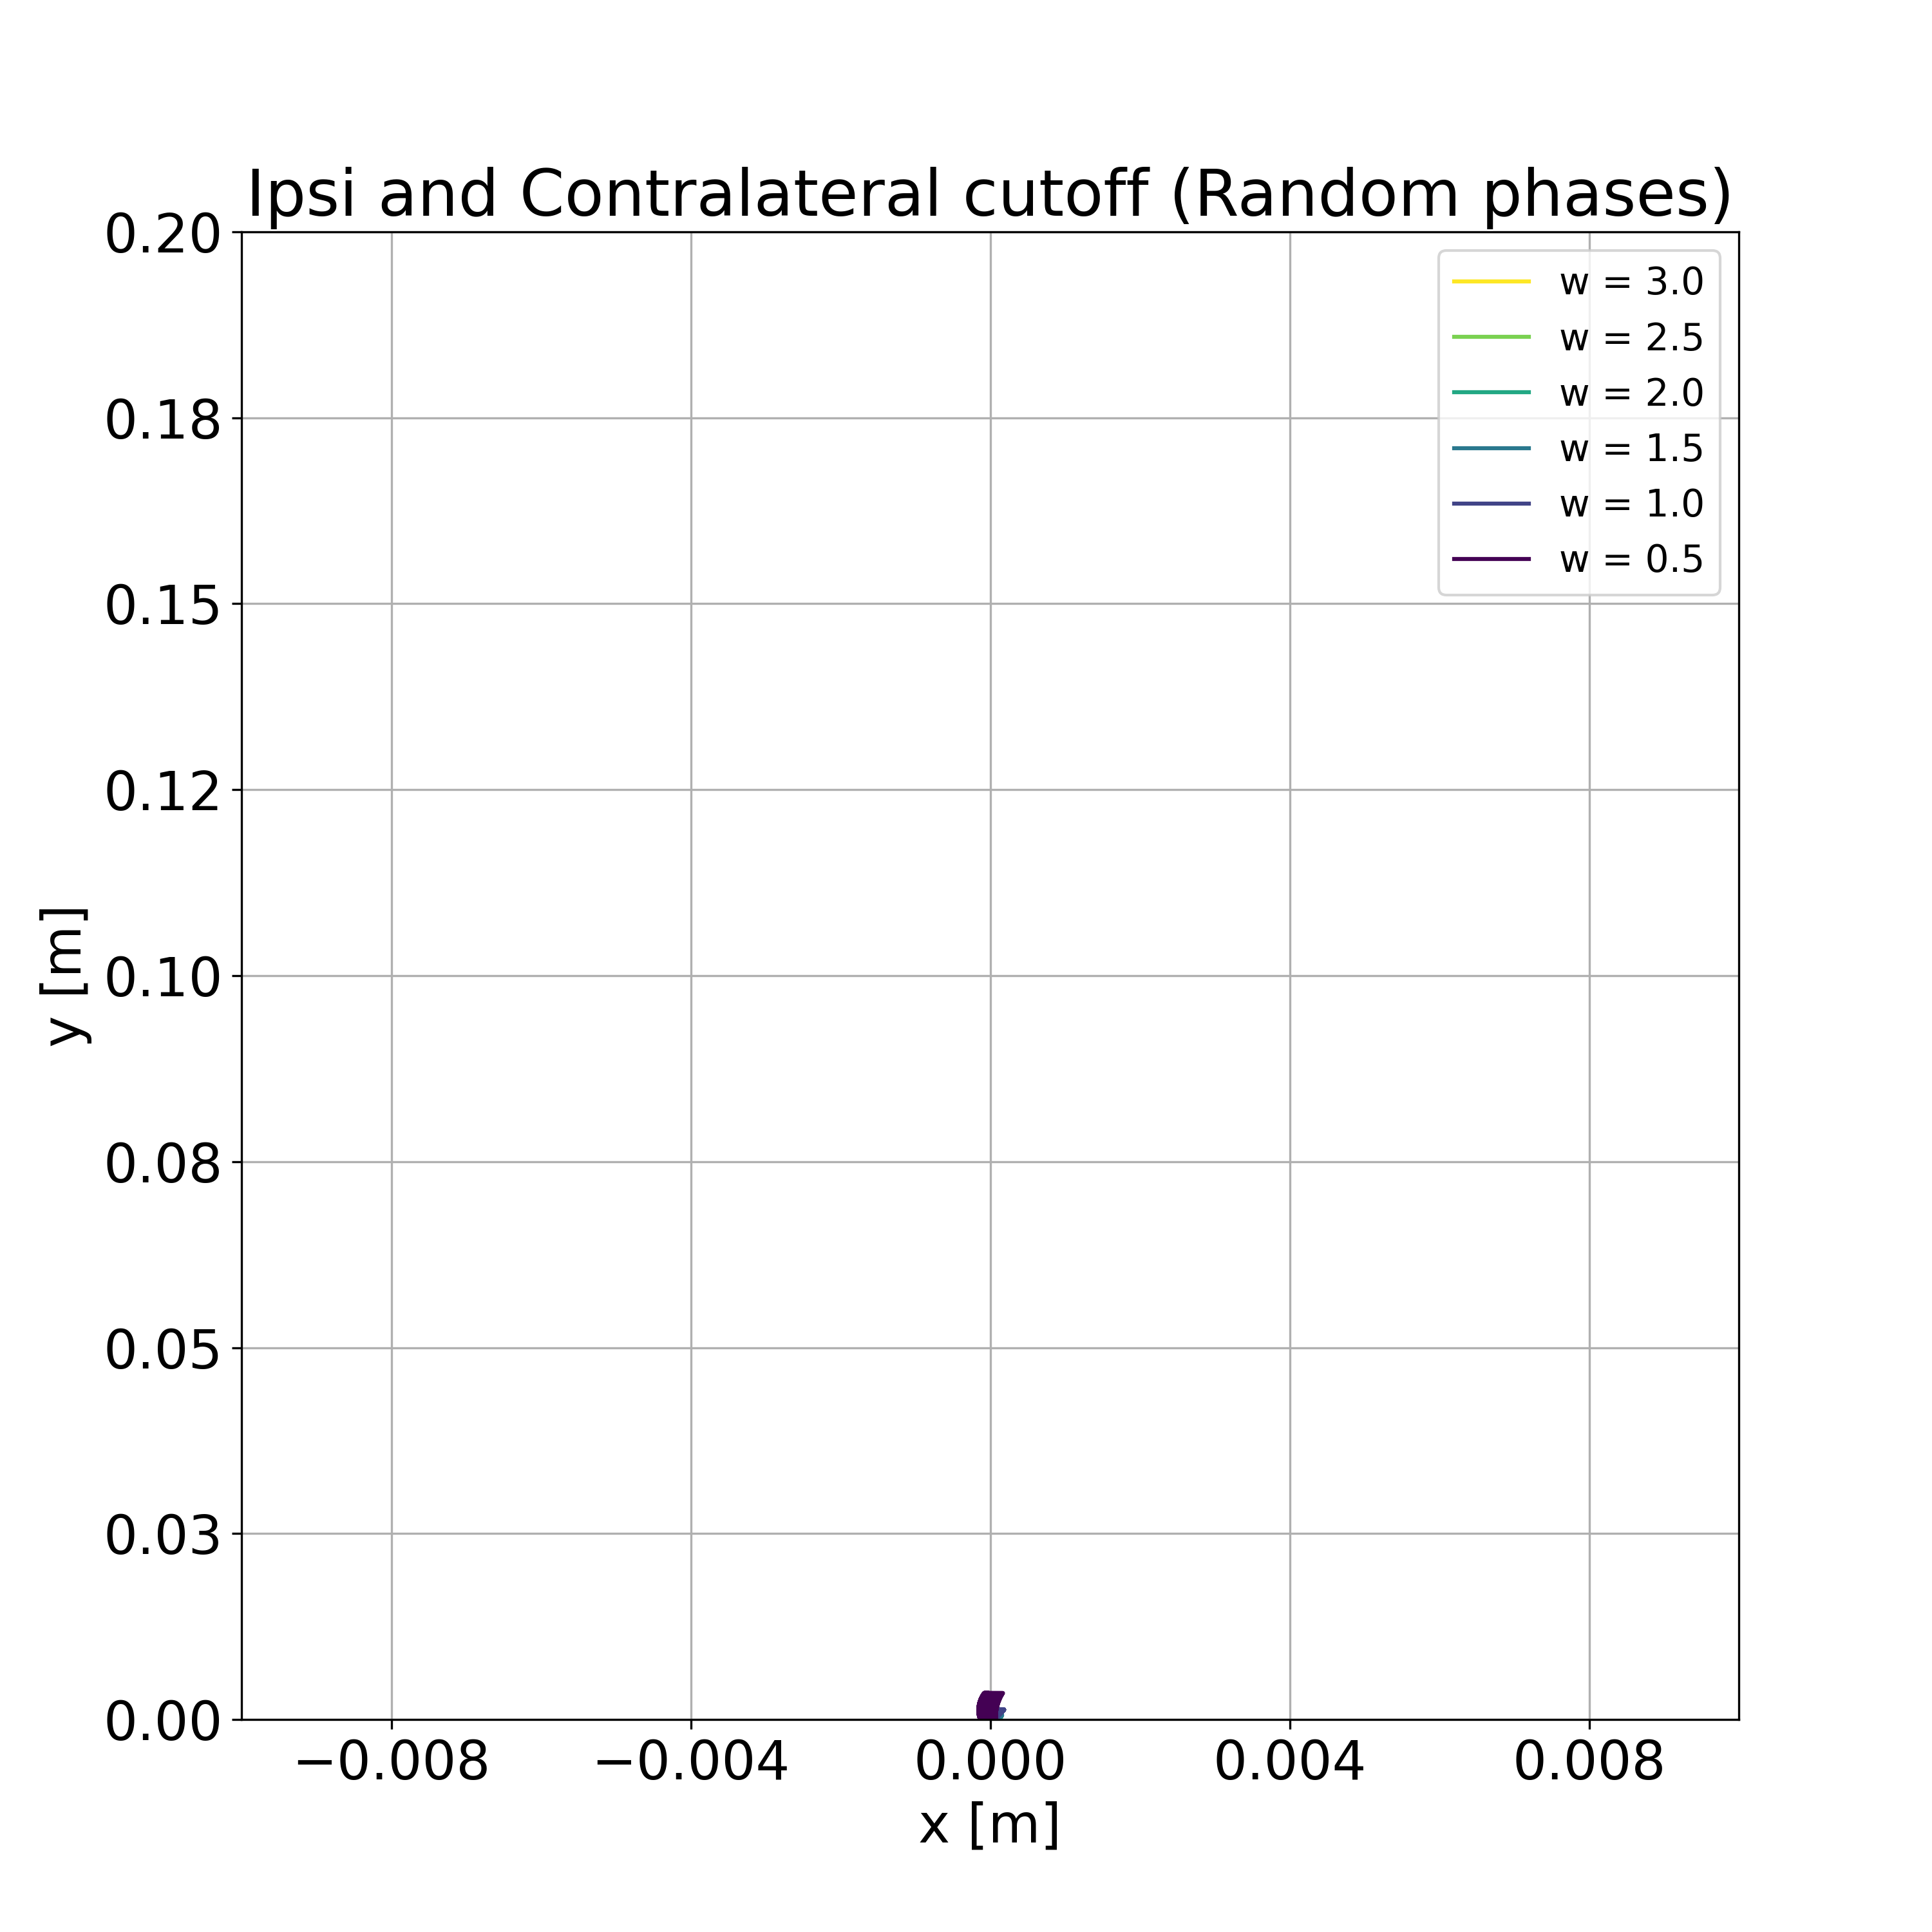
\includegraphics[width=\linewidth]{our_figures/Ipsi and Contralateral cutoff_random.png}
        \caption{Trajectory of the fish's head under ipsilateral and contralateral impairment for different feedback gain $w$.}
        \label{fig:contra_ipsi_cutoff}
    \end{subfigure}
    \caption{Comparison of fish head trajectories under different impairment conditions (random initial phases).}
    
\end{figure}

Looking at Figure 15, we see that a contralateral connection strength of 4 is enough to initialize the gait with normal speed. However, just like we saw with contralateral impairment, the trajectory still shifts heavily to one side. Since there’s no clear definition of what counts as a “correctly initialized” gait in terms of directional stability, we assume that a strength of 8 or 9 is enough, as it only causes a small shift in direction. So, depending on what the goal is, whether it’s just swimming speed or also a stable trajectory, a strength of 4 might be enough for the former, but around 8 or 9 is needed for the latter.

\begin{figure}[H]
    \centering
    \begin{subfigure}[t]{0.48\linewidth}
        \centering
        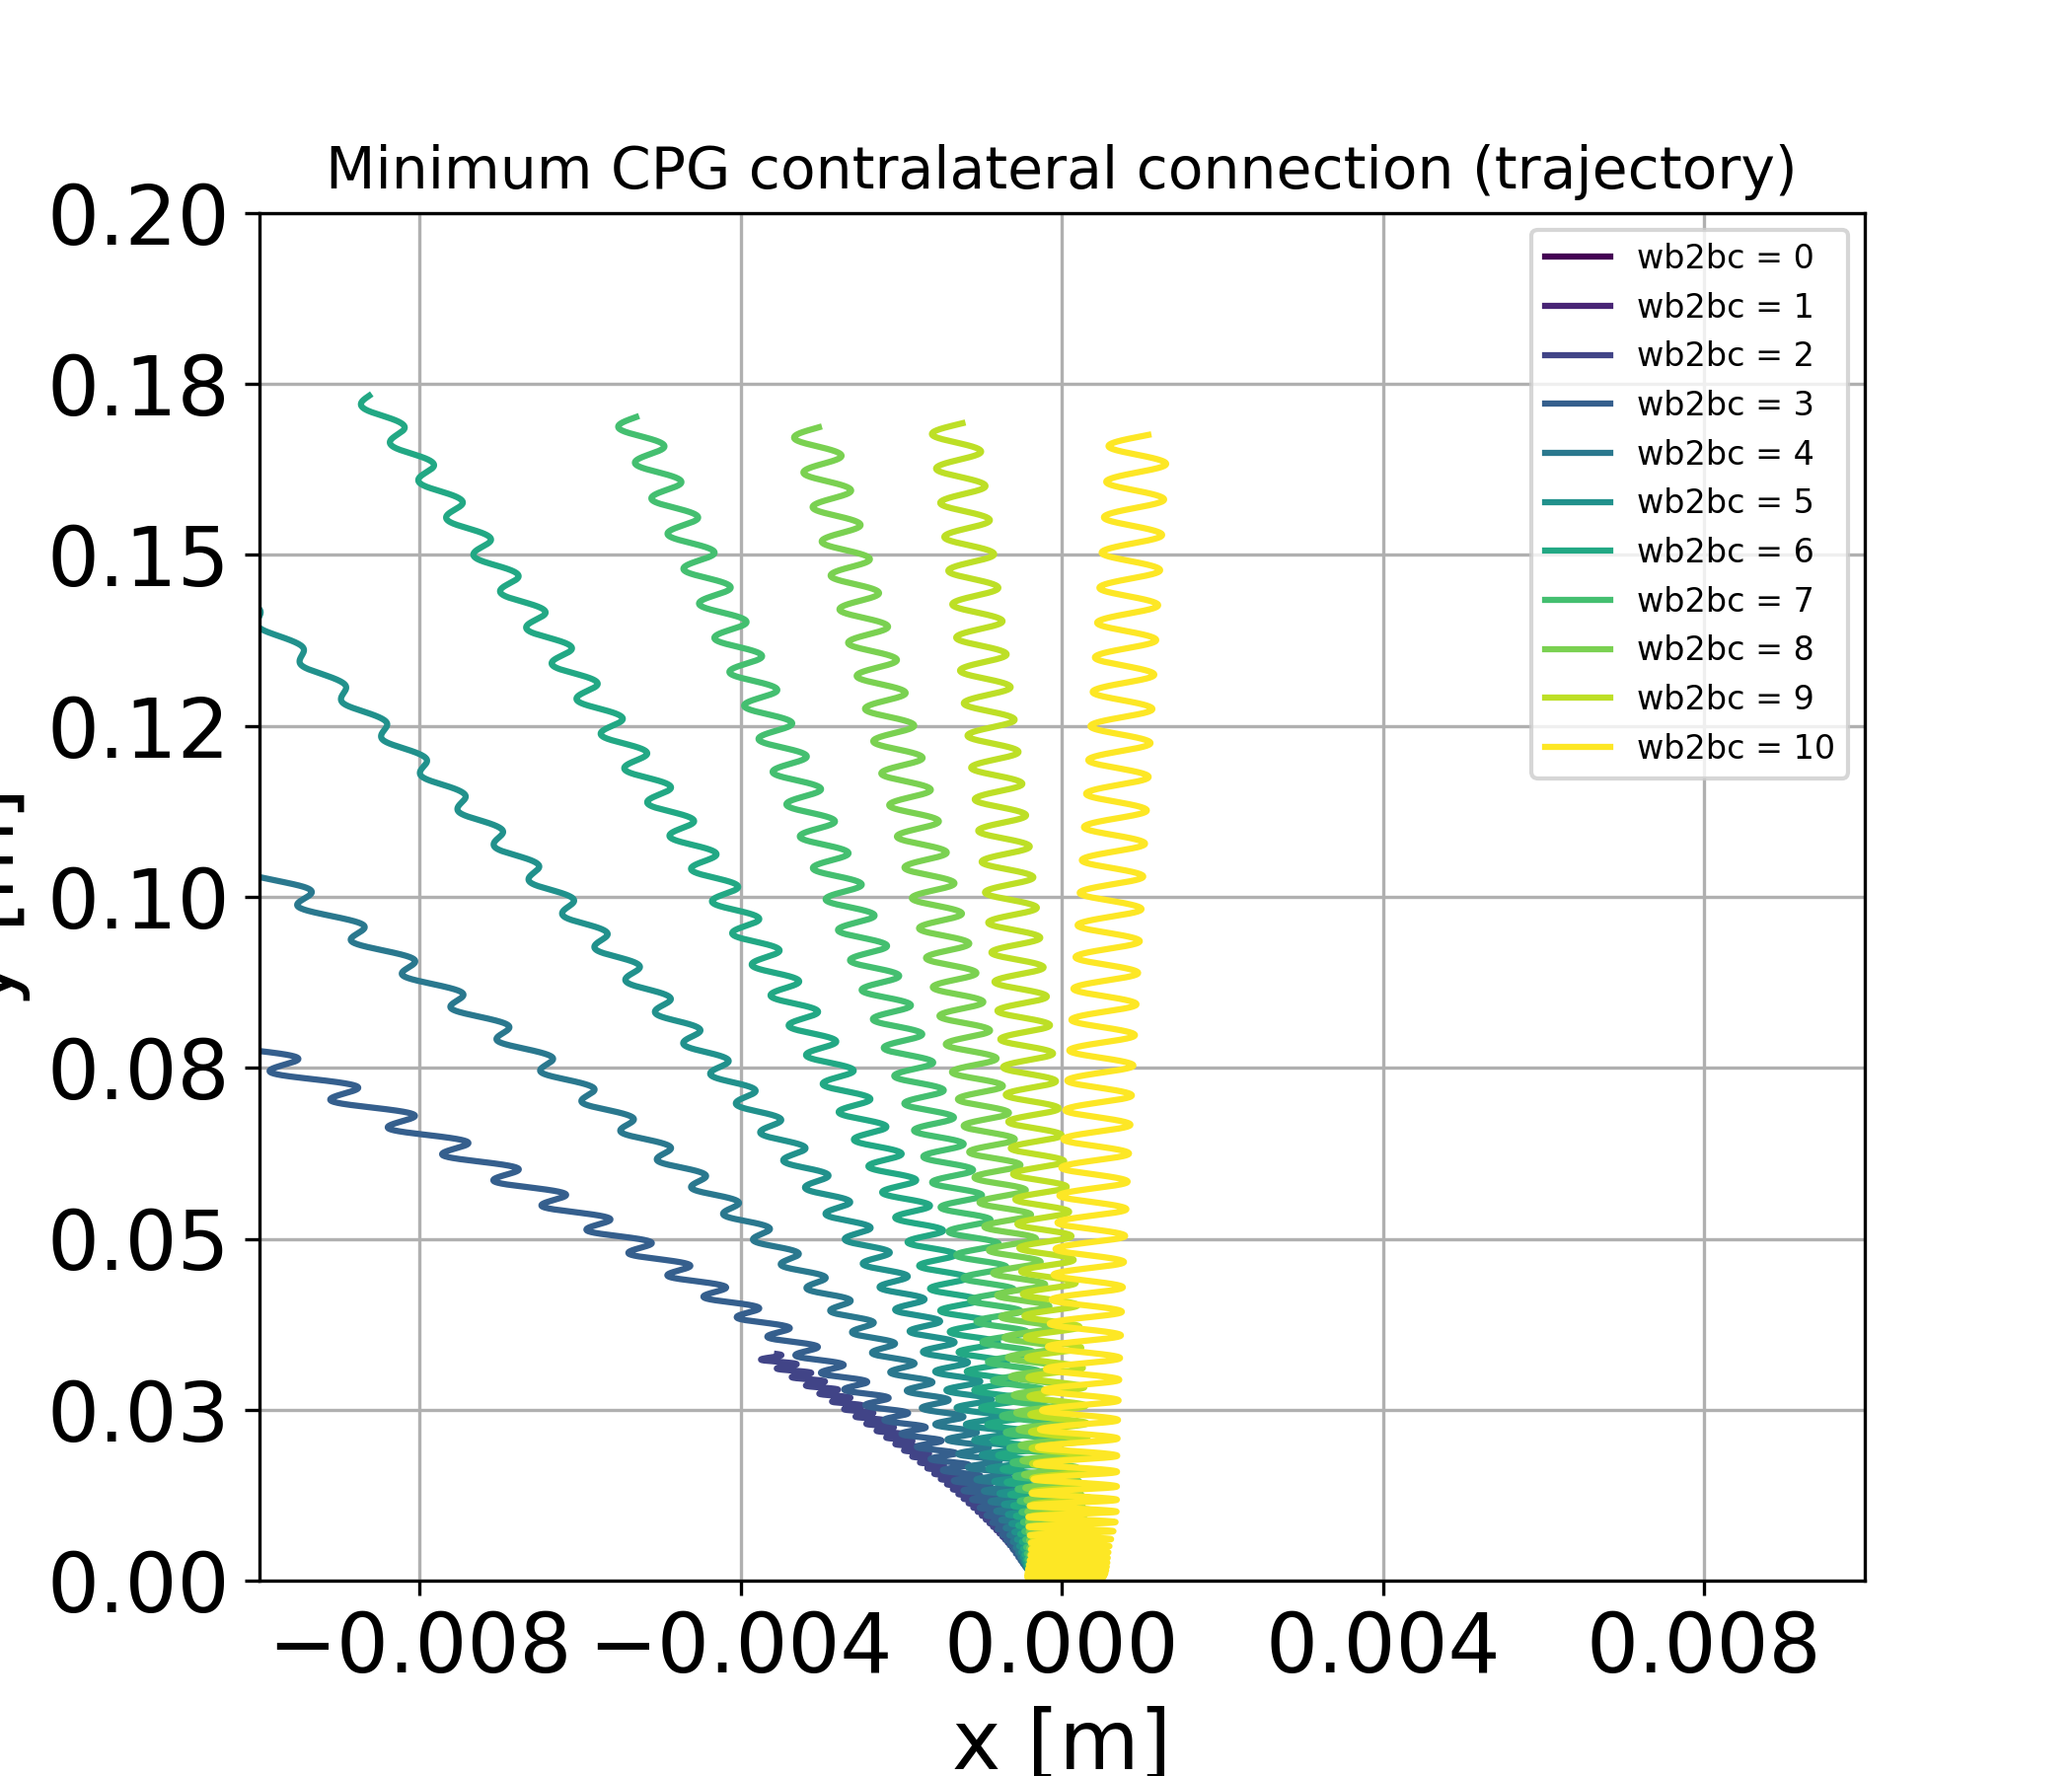
\includegraphics[width=\linewidth]{our_figures/min_contralateral_connections_trajectory.png}
        \caption{Trajectory of the fish's head for different contralateral connections strenghts $w$.}
        \label{fig:contra_strenght_traj}
    \end{subfigure}
    \hfill
    \begin{subfigure}[t]{0.48\linewidth}
        \centering
        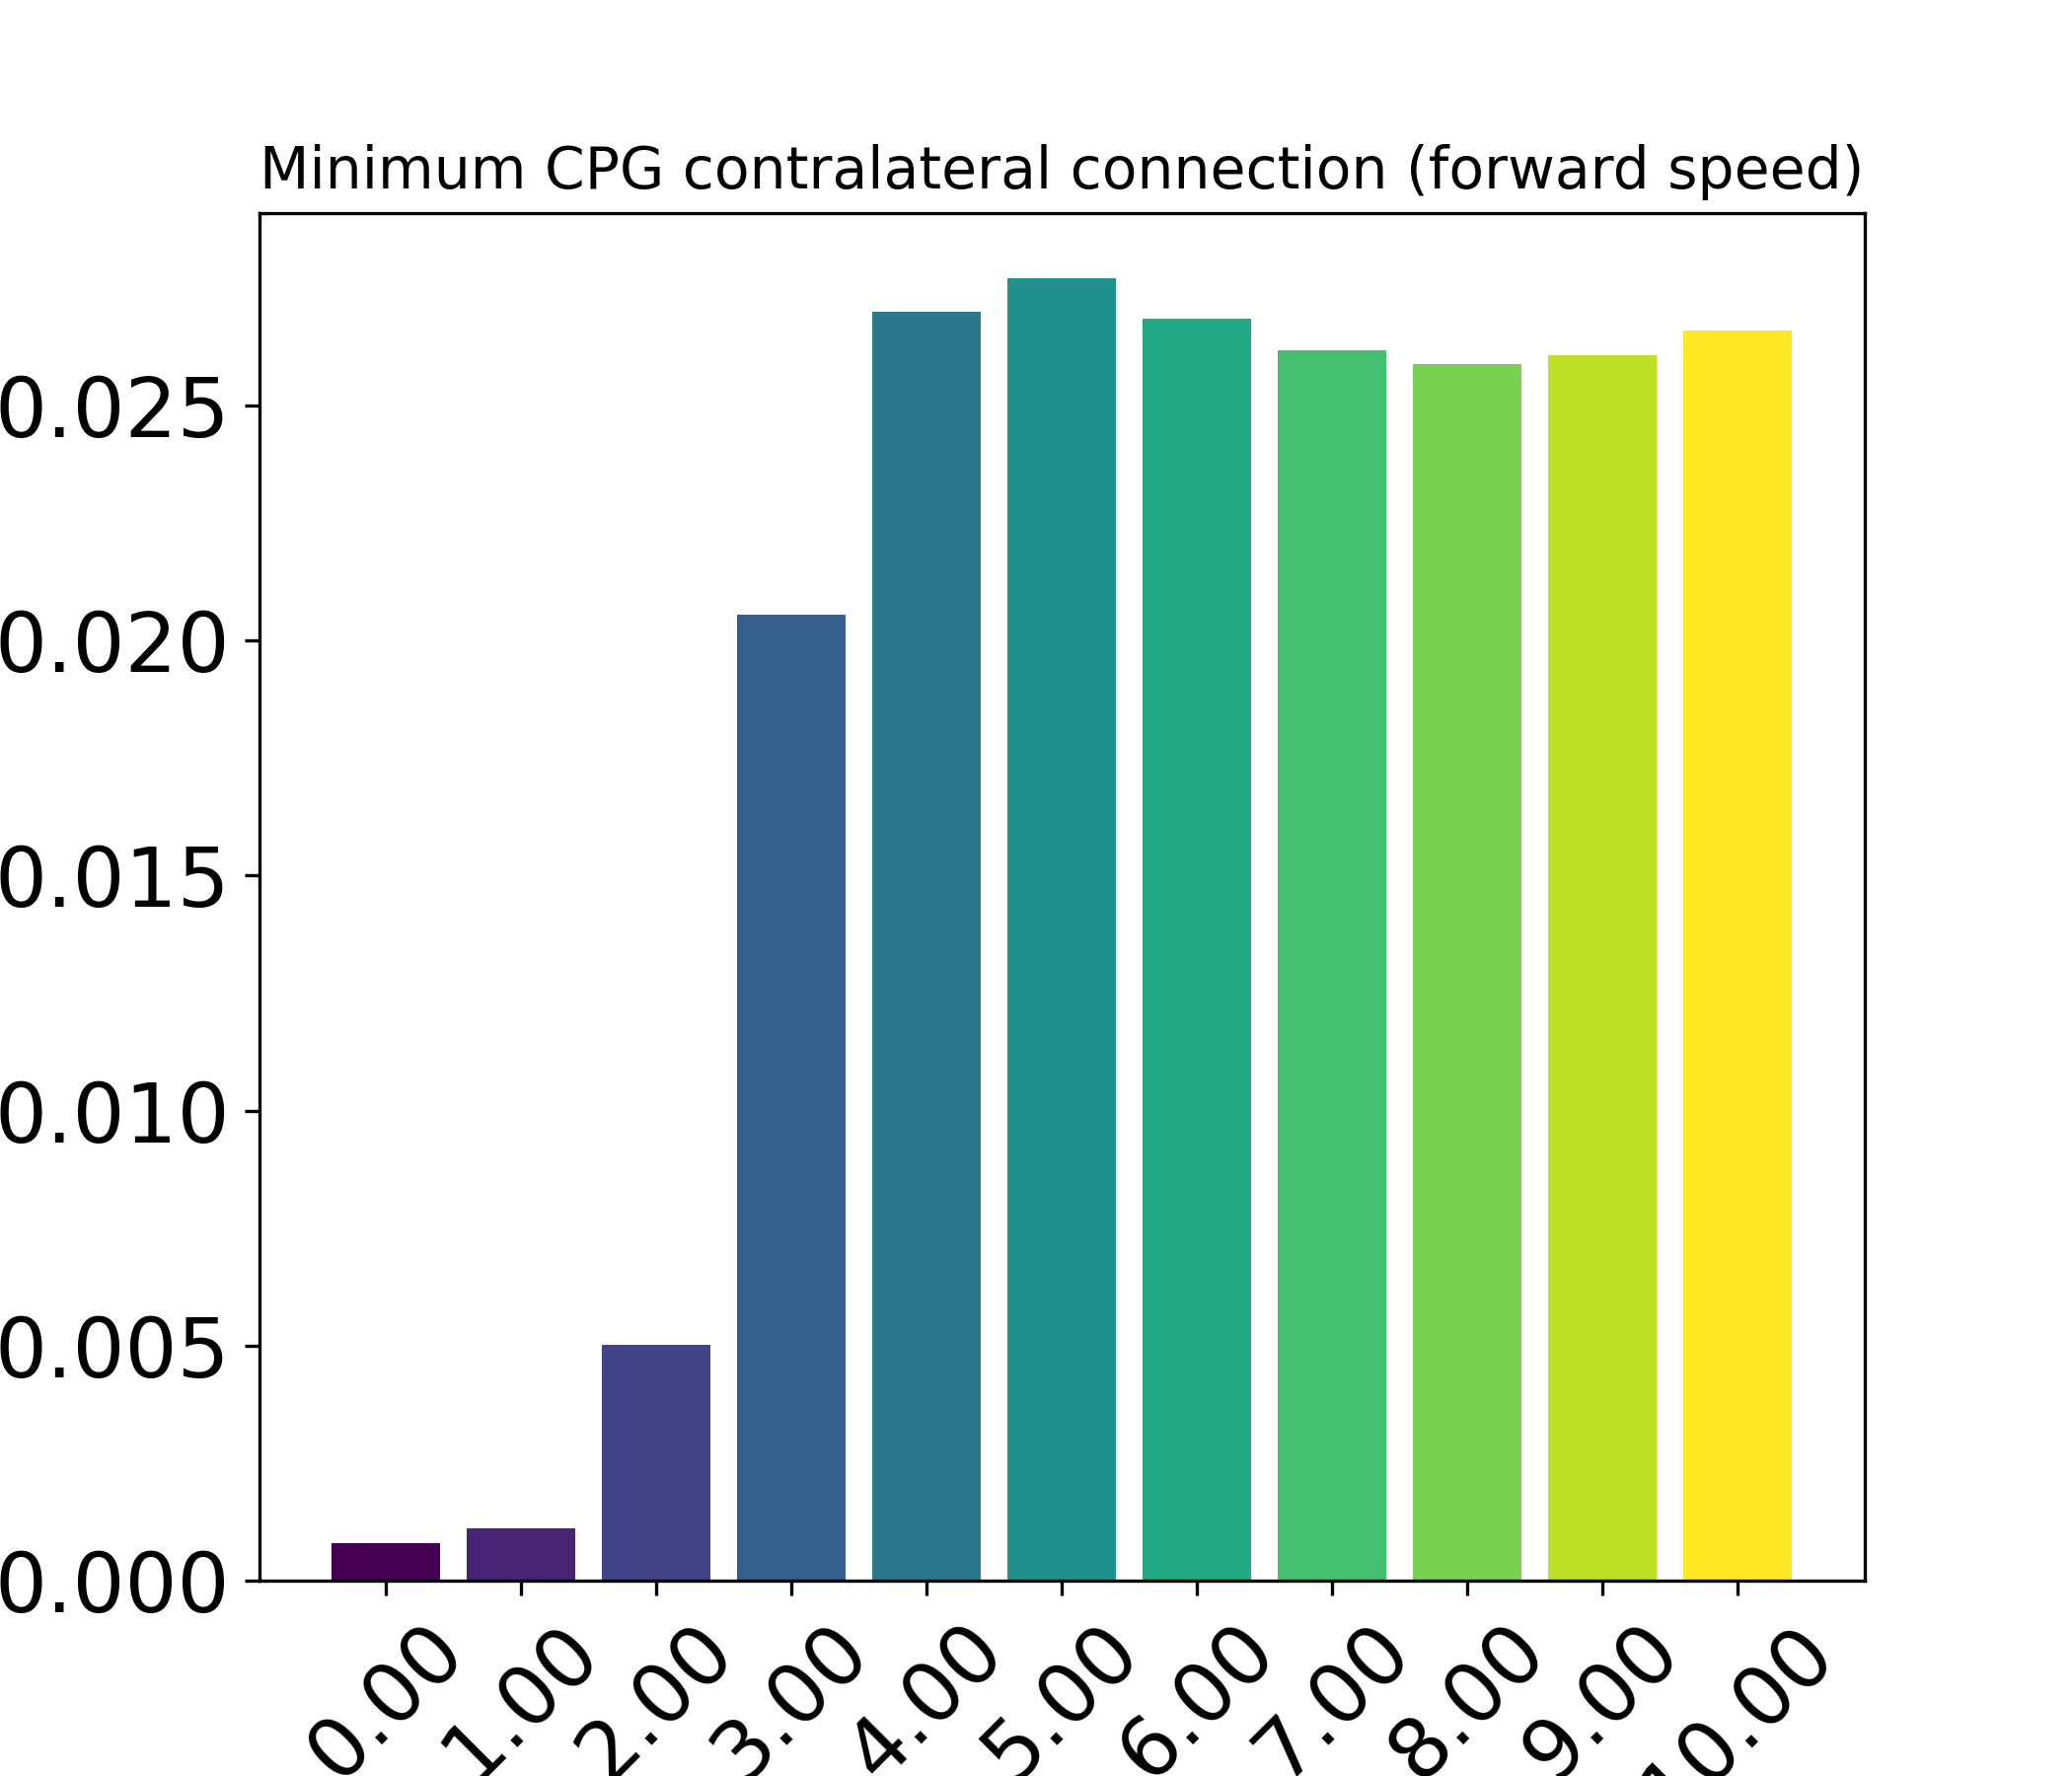
\includegraphics[width=\linewidth]{our_figures/min_contralateral_connections_speed.png}
        \caption{Forward speed of the fish's for different contralateral connections strenghts $w$.}
        \label{fig:contra_strenght_speed}
    \end{subfigure}
    \caption{Comparison of fish head trajectories under different impairment conditions (random initial phases, feedback strenght w=2).}
    
\end{figure}



%% -----------------------------SOLUTION ------------------------------


\bibliographystyle{ieeetr}
\bibliography{cmc_2025}
\label{sec:references}





% \newpage

% \section*{APPENDIX}
% \label{sec:appendix}

\end{document}

%%% Local Variables:
%%% mode: latex
%%% TeX-master: t
%%% End: